\documentclass[conference]{IEEEtran}
\IEEEoverridecommandlockouts

\usepackage{cite}
\usepackage{amsmath,amssymb,amsfonts}
\usepackage{algorithmic}
\usepackage{graphicx}
\usepackage{textcomp}
\usepackage{xcolor}
\usepackage{tabularx}
\usepackage{minted}
\usepackage{graphicx}
\usepackage[hidelinks]{hyperref}

\usemintedstyle{borland}

\newcommand{\chameleon}{ChameleonIDE}
\newcommand{\pjs}[1]{\textcolor{blue}{\textsc{Pjs}: #1}}
\newcommand{\jw}[1]{\textcolor{orange}{\textsc{JW}: #1}}
\newcommand{\td}[1]{\textcolor{teal}{\textsc{td}: #1}}
\newcommand{\tf}[1]{\textcolor{magenta}{\textsc{tf}: #1}}

\def\BibTeX{{\rm B\kern-.05em{\sc i\kern-.025em b}\kern-.08em
    T\kern-.1667em\lower.7ex\hbox{E}\kern-.125emX}}

\newcommand{\ignore}[1]{}    
    
\begin{document}

\title{\chameleon{}: Untangling Type Errors Through Interactive
  Visualization and Exploration
}

\ignore{
\author{\IEEEauthorblockN{1\textsuperscript{st} Given Name Surname}
\IEEEauthorblockA{\textit{dept. name of organization (of Aff.)} \\
\textit{name of organization (of Aff.)}\\
City, Country \\
email address or ORCID}
\and
\IEEEauthorblockN{2\textsuperscript{nd} Given Name Surname}
\IEEEauthorblockA{\textit{dept. name of organization (of Aff.)} \\
\textit{name of organization (of Aff.)}\\
City, Country \\
email address or ORCID}
\and
\IEEEauthorblockN{3\textsuperscript{rd} Given Name Surname}
\IEEEauthorblockA{\textit{dept. name of organization (of Aff.)} \\
\textit{name of organization (of Aff.)}\\
City, Country \\
email address or ORCID}
\and
\IEEEauthorblockN{4\textsuperscript{th} Given Name Surname}
\IEEEauthorblockA{\textit{dept. name of organization (of Aff.)} \\
\textit{name of organization (of Aff.)}\\
City, Country \\
email address or ORCID}
\and
\IEEEauthorblockN{5\textsuperscript{th} Given Name Surname}
\IEEEauthorblockA{\textit{dept. name of organization (of Aff.)} \\
\textit{name of organization (of Aff.)}\\
City, Country \\
email address or ORCID}
\and
\IEEEauthorblockN{6\textsuperscript{th} Given Name Surname}
\IEEEauthorblockA{\textit{dept. name of organization (of Aff.)} \\
\textit{name of organization (of Aff.)}\\
City, Country \\
email address or ORCID}
}
}

\maketitle

\begin{abstract}
In recent years, many programming communities have been undergoing a transition to writing strongly typed programs. To benefit from type-safe codebases, programmers must first overcome the challenge of resolving type errors where text messages can often be unhelpful and misleading. Modern programming tools do not concentrate on making type errors easy to understand. We demonstrate \chameleon{}, a type debugging tool capable of displaying the full context of a type error and allowing programmers to search for where the type error actually occurs based on their prior knowledge and to incrementally verify their assumptions. \chameleon{} was developed through a user-centered, iterative process with four participatory experiments. Through the experiments, we showed that programmers using \chameleon{} fix type errors faster than traditional text-based error messages.  This difference is more significant in harder tasks. Further, programmers actively using \chameleon{} interactive features are shown to be more efficient in fixing type errors than simply reading the type error output.
\end{abstract}

\begin{IEEEkeywords}
component, formatting, style, styling, insert
\end{IEEEkeywords}





% \todo{As above, would start with motivation of dynamically typed langs e.g. JavaScript, Pythjon popularity but issues this brings...
% }

Dynamically typed programming languages such as JavaScript and Python have risen in popularity in recent decades \cite{chatley_next_2019}. These languages present a low barrier of entry, especially to beginner programmers: they require no type declaration, variable types or object structures can be modified dynamically, and functions can deal with dynamic input using ad-hoc polymorphism and runtime reflection. However, studies show that dynamically typed languages negatively affect development productivity \cite{kleinschmager_static_2012}, code usability \cite{mayer_empirical_2012}, and code quality \cite{gao_type_2017, ray_large-scale_2017, meyerovich_empirical_2013}. They are often found to produce error-prone code \cite{chen_empirical_2020, wang_empirical_2015,xu_python_2016} and require strong programmer discipline to avoid pitfalls \cite{chen_empirical_2020}. For these reasons, many modern dynamically-typed languages have introduced static typing annotations as part of the core language features in recent years (e.g.\ \textit{TypeScript}~\cite{microsoft_javascript_nodate} and \textit{mypy}~\cite{mypy_mypy_nodate}).

Functional programming languages have long enjoyed rigorous type systems and expressive type-level features. Techniques such as type inference and algebraic types have been standard practice for decades in functional languages such as ML and Haskell, and more recently in multi-paradigm languages, such as Rust and TypeScript. Various type system advances were introduced in Haskell and ended up in mainstream languages years or even decades after, leading many to consider Haskell the ``type-system laboratory" \cite{hudak_history_2007}.  Type classes, an implementation of generic programming, were introduced to Haskell in 1988~\cite{hudak_history_2007}, and now can be found in most popular languages such as C\#~\cite{bill_wagner_constraints_2022}, Java~\cite{oracle_generic_2022}, and TypeScript~\cite{microsoft_documentation_2022}.

One crucial challenge of programming in statically-typed languages is that type errors can sometimes be difficult to resolve~\cite{tirronen_understanding_2015, hage_solved_2020}. In particular, they may point to locations that are not the root  causes of the type error, expose errors in cryptic language, or provide misleading fixing suggestions~\cite{wu_how_2017}.
% Compared to dynamic type systems, static type systems offer programmers opportunities to weed out a large number of errors at compile time (reducing the need for run-time debugging) and to increase usability~\cite{mayer_static_2012} and codebase maintainability~\cite{kleinschmager_static_2012}. In recent years, the programming community has seen a trend of migrating away from dynamically typed codebases due to the lack of maintainability and refactoring safety when systems reach large scale and complexity~\cite{chatley_next_2019}. These migration methods include the introduction of gradual type annotations (e.g., JavaScript to TypeScript or Python with mypy) or transition to a modern strongly-typed language (Scala, Rust, Haskell, PureScript, etc.). However, with dynamically typed languages (e.g., JavaScript, PHP, and Python) still being most peoples' formative experience with programming and with such languages now firmly entrenched in education~\cite{stackoverflow_stack_2022}, this transition may pose difficulties for programmers who lack experience writing type-safe programs.

% \todo{There are a lot of minor grammer fix-ups needed throughout...}
% Programmers find challenges in adopting typed languages in their practice. \todo{I think this statement is plain wrong myself... 
%  Need strong references to justify if going to say this to SE audience!:}They tend to be verbose, hard to learn and generate bad error messages. 
% One obstacle programmers face when using a statically typed language is understanding and resolving type errors~\cite{marceau_measuring_2011, tirronen_understanding_2015}, especially when dealing with modern type features such as polymorphic types and implicit typing. Studies show most statically typed languages produce unhelpful and even misleading type errors~\cite{}. Symptoms of bad error messages include cryptic language exposing internal constructs of the compiler and incomplete or wrong error locations. These usability issues pose challenges to learners and teachers of the languages. impede the wide adoption of statically typed languages, especially for programmers who are now accustomed to the mindset of writing un-typed programs.

This paper introduces \chameleon{}, an interactive type debugging tool for Haskell. It can visualize the relevant context of a type error: where it happens or could have happened and which parts of the code cause it. In addition, \chameleon{} allows programmers to interactively explore all the parts of code where multiple types can be inferred and to resolve ambiguity. The most noticeable features are the type compare tool (Section \ref{sub:type-compare}), the candidate expression card (Section \ref{sub:candidate-expression}), and the deduction step (Section \ref{sub:deduction-steps}). These features are integrated into a debugging environment and can be enabled or disabled separately based on the programmers' preferences and debugging needs. \chameleon{} is open-source and is available at ~\cite{anonymous_chameleon_2022}.  
% \todo{Introduce Haskell earlier?  Motivate WHY Haskell?} The current implementation of \chameleon{} targets the Haskell 2010 language standard. However, it is planned to extend it to support other programming languages using the same underlying ideas and techniques. Historically, Haskell has been a test bed for advanced language features, and it is common for features established in Haskell to be transferred to mainstream programming languages. 

% \chameleon{} uses underlying type inference algorithms adapted from the command-line tool, Chameleon, developed in 2005 \cite{chameleon}. As described in Section \ref{sec:typeinferenceengine}, Chameleon computes the Minimum Unsatisfiable Subset (MUS) \tf{Explain what mus is} of type constraints in order to identify a set of code locations where multiple types can be inferred. Compared to standard compiler messages, which arbitrarily report the first place a type conflict arises, Chameleon error messages give a lot more context to the programmer to help them correctly resolve the conflict to match the program's intent. However, the Chameleon system was never tested with users.  Therefore, the first contribution of this paper is to address the research question: \textit{Is a minimally interactive version of Chameleon's multipart type-conflict display more effective in supporting type error debugging than traditional error messages? } (Sections~\ref{sub:us1} and \ref{sub:us2}).

% After affirming that the information Chameleon provides is beneficial for more complex type errors, we ask \textit{Do programmers benefit from the interactive exploration of type error locations?} (Sections~\ref{sub:us3} and \ref{sub:us4}). We then explore \textit{How do programmers use the interactive exploration features to solve type errors?}  (Section~\ref{sub:us4}).


This paper makes the following contributions:
\begin{itemize}
\item We provide the design and implementation of the \chameleon{} to visualize the relevant context of a type error and allow programmers to explore and verify the error locations in small chunks interactively.  
\item {
    We report the results of three experiments designed to evaluate \chameleon{}.}
\end{itemize}

Our experiments showed that programmers using \chameleon{} fix type errors faster than with traditional text-based error messages. This difference is more significant when solving harder tasks. Further, programmers who actively use \chameleon{} interactive features fix type errors faster than simply reading the type error output. Although \chameleon{} is designed to work with
the Haskell language, we plan to extend the underlying ideas to work with other strongly typed languages.
\section{Related Work}

Researchers have long realized that incomprehensible type errors result as a consequence of standard approaches to the type inference process. Haack and Wells~\cite{haack2004type} noted that ``\textit{Identifying only one node or subtree of the program as the error location makes it difficult for programmers to understand type errors. To choose the correct place to fix a type error, the programmer must find all the other program points that participate in the error.}'' Researchers have proposed solutions to improve the type inference process. Type error slicing~\cite{haack2004type} is a technique that finds locations that are complete and minimal for the type error. Internally labeled constraints and MUS manipulation are used to generate these slices. The language supported in Haack's work was a subset of standard ML. The original Chameleon~\cite{stuckey2003interactive} used a similar technique but extended it to support advanced type-level features (type classes and functionally dependent types). The project also introduced the ability to query type information through a command line-style interface (Fig.~\ref{fig:original-chameleon}). Although Chameleon was firmly grounded in results from type theory, its designs were never evaluated with user studies.


% \begin{figure}[h]
%     \centering
%     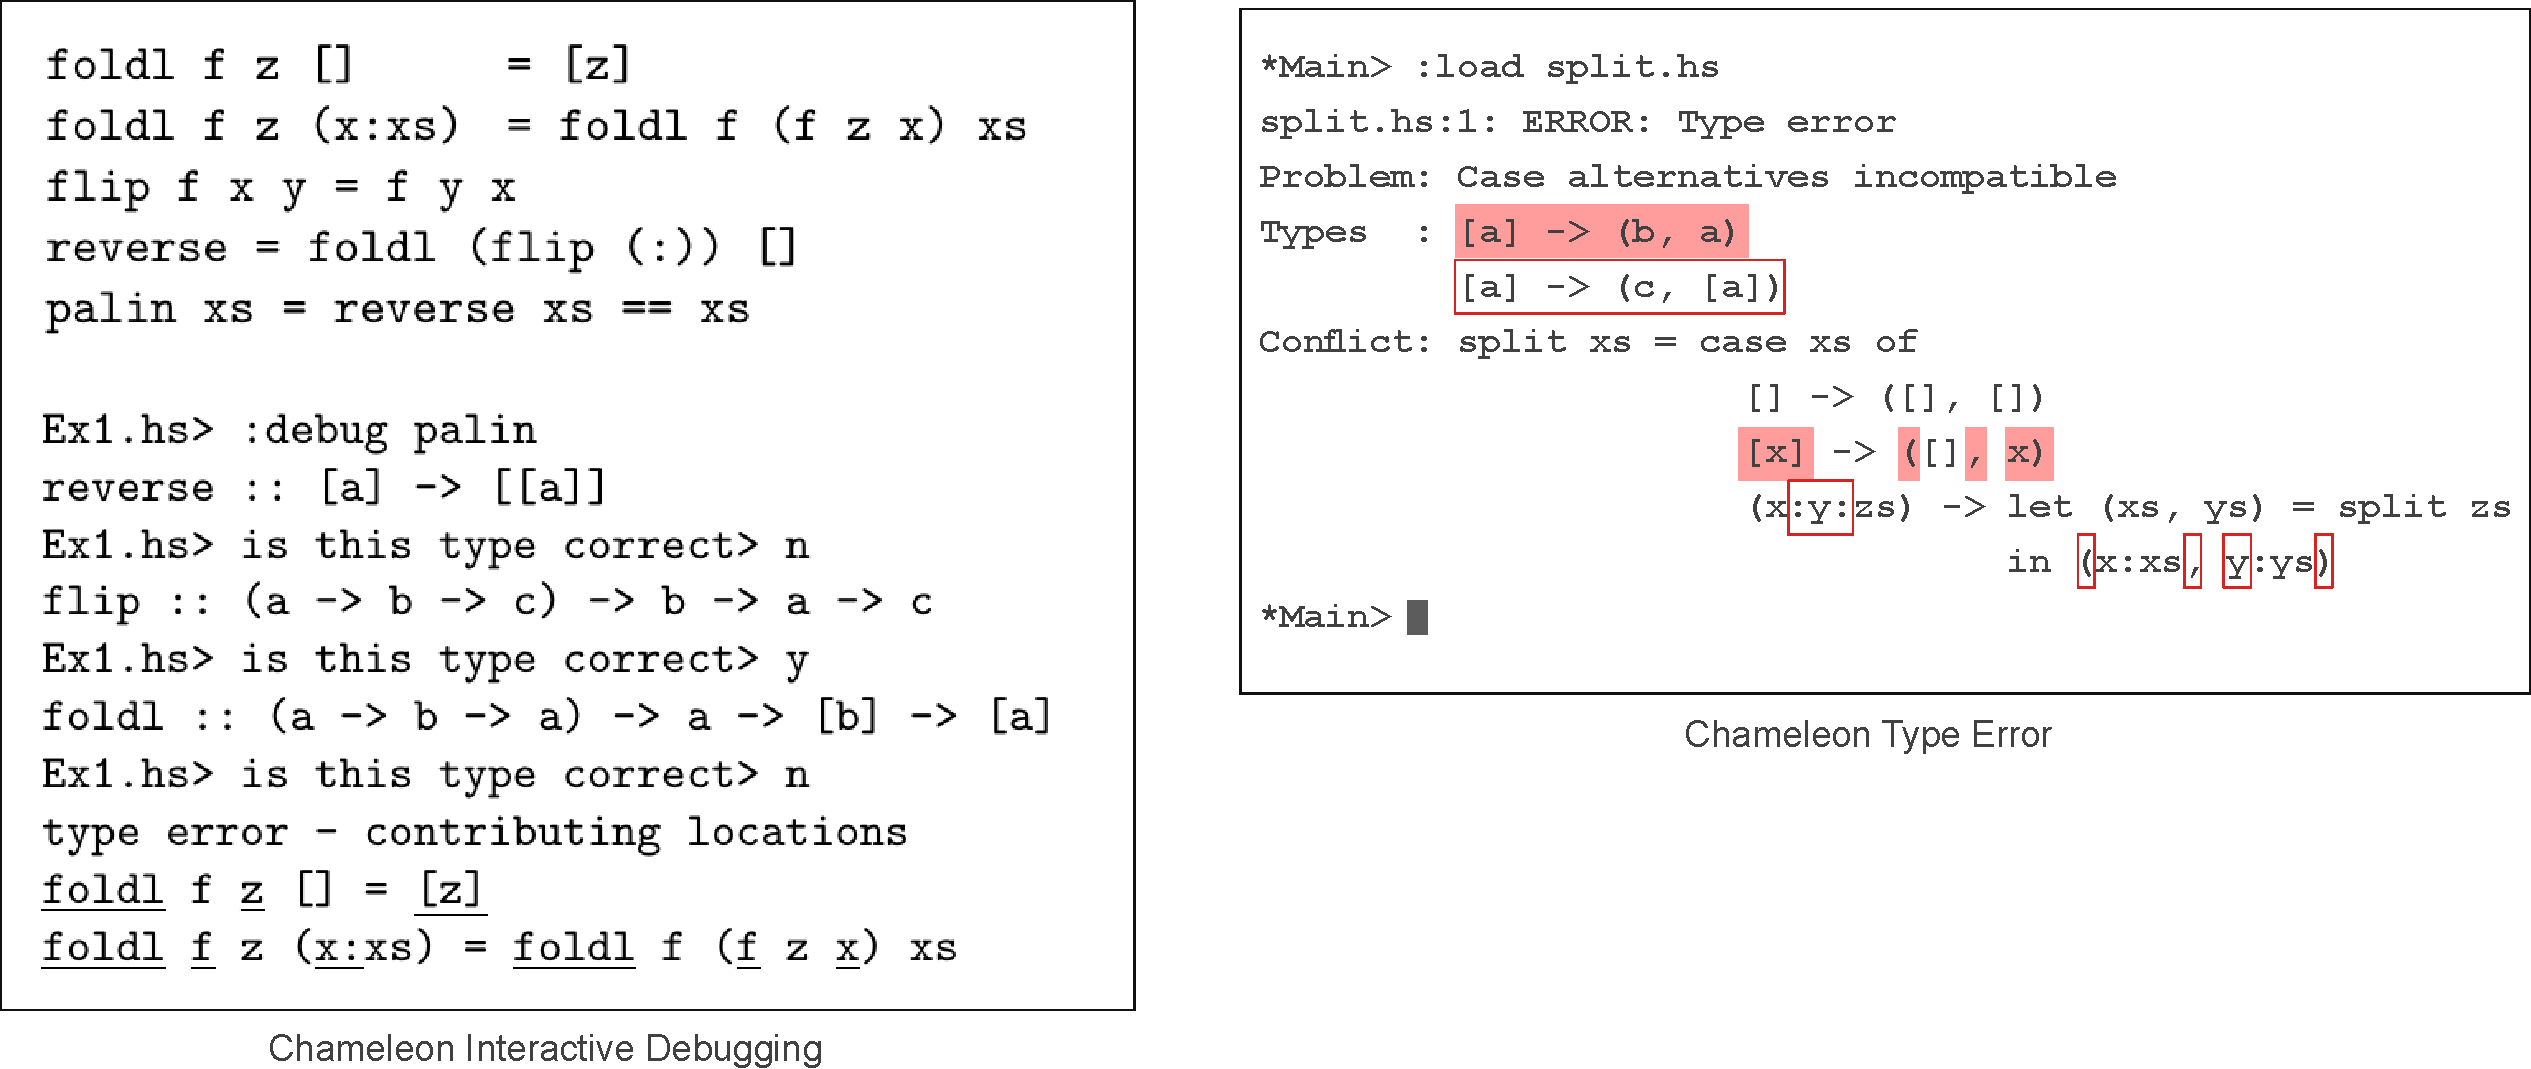
\includegraphics[width=\linewidth]{images/original-chameleon.pdf}
%     \caption{
% Originally, Chameleon was a command-line tool that can list all the potential causes of a type error and display the two branches in two forms of highlight (right), achieved with ASCII colors. In addition, it allows a few commands (debug and explain) in the debugging shell to help debug type errors (left).}
%     \label{fig:original-chameleon}
% \end{figure}


% The ChameleonIDE error reporting The error message of ChameleonIDE closely
% follows the argumentation structure outlined by Titus. Basic mode represent a
% simple structure argument, where the claim "The expression e can have two
% conflicting types" and the possible type 1 and two serves as grounds. When
% inspecting each possible types, the type judgements are treated as claim, and it
% is supported by the grounds: "Inferred from the orange/blue highlights on the
% left side". On the other hand, the similar type error message in GHC "Couldn't
% match expect type T1 with actual type T2" is "a ground masquerading as a clam",
% Barik commented. The balanced mode and advanced mode serve as a way to elaborate
% arguments from simple arguments into extended arguments.

Another related topic is type-explanation~\cite{yang1999explaining, jun2002explaining}. Yang~\cite{jun2002explaining} showed an alternative type inference system capable of producing a human-like text explanation for why expressions are assigned certain types. A good explanation is drawn from surveying how human experts explain types. The resulting algorithm $\mathcal{H}$, generates a succinct explanation of the type inference steps to avoid using internal constructs (such as type variables). The explanation system has the advantage of acting like a human expert. However, when presented as text-based output, explanation systems have the potential to become verbose when types are complex or variable names are long. In \chameleon{}, we attempt to address this problem by showing one step of explanation at a time and referring to variables instead of spelling out the full name.

% Another method to improve type error message is search based type
% checking~\cite{lerner2007searchingtypeerror}. This method incrementally modifies
% an ever smaller part of the abstract syntax tree and replacing it with a
% wildcard expression and querying the type checker to verify if the program still
% type-checks. Lerner's study showed how two implementations could provide
% high-quality error messages and to suggest accurate fixes. While this system is
% great for suggesting solutions, is it limited in its ability to explain the type
% errors due to the fact that the system is unaware of any inner workings of the
% type systems. 


% Some studies \cite{seidel2017learningtoblame} proposed a heuristic approach to
% improve type error messages. These studies use part of type information in the
% program to query external databases. Based on the external databases'
% capability, some projects can interactively fix the type error on the fly with
% reasonable accuracy. \pjs{Add jusdgment/comparison sentence!}



Debugging using a GUI Interactive Development Environment has been the standard practice for a very long time. Compared to a command line-based interface, a graphic user interface provides programming tools with the ability to show information hierarchy, provide immediate feedback to changes, and display complex visualizations. RxFiddle~\cite{banken2018debugging} is a tool to visualize data flow and value changes in a functional reactive program. Whyline~\cite{ko2009finding} is a Java debugging system that allows a user to ask questions like "why does variable X have value Y". It also allows users to interactively ask follow-up questions to gain further knowledge of the nature of an error. Both  systems target programming runtime systems instead of types systems and static analysis. In fact, support for type systems has been lacking in both academic and industry software engineering tool design. The most common approach for supporting type systems we see in current programming editors and IDEs is to display type annotations when hovering on an expression and show a squiggly line to indicate the type error location. In \chameleon{}, colours and geometric shapes are used to create visual clarity of different components of a type error; interactivity is used to show conditional information and to change the granularity of details.




\section{Motivation}
The design requirements of \chameleon{} are motivated by limitations of traditional type errors, as documented in a number of studies (e.g.~\cite{yang_improved_2000, hage_solved_2020}), but which we illustrate here with a few motivating examples. 
%These limitations are sourced from the authors' frustration in teaching and writing Haskell. This list of shortcomings of traditional type errors is also strengthened by multiple studies pursuing improvement\cite{yang_improved_2000}. 

\begin{figure}
    \centering
    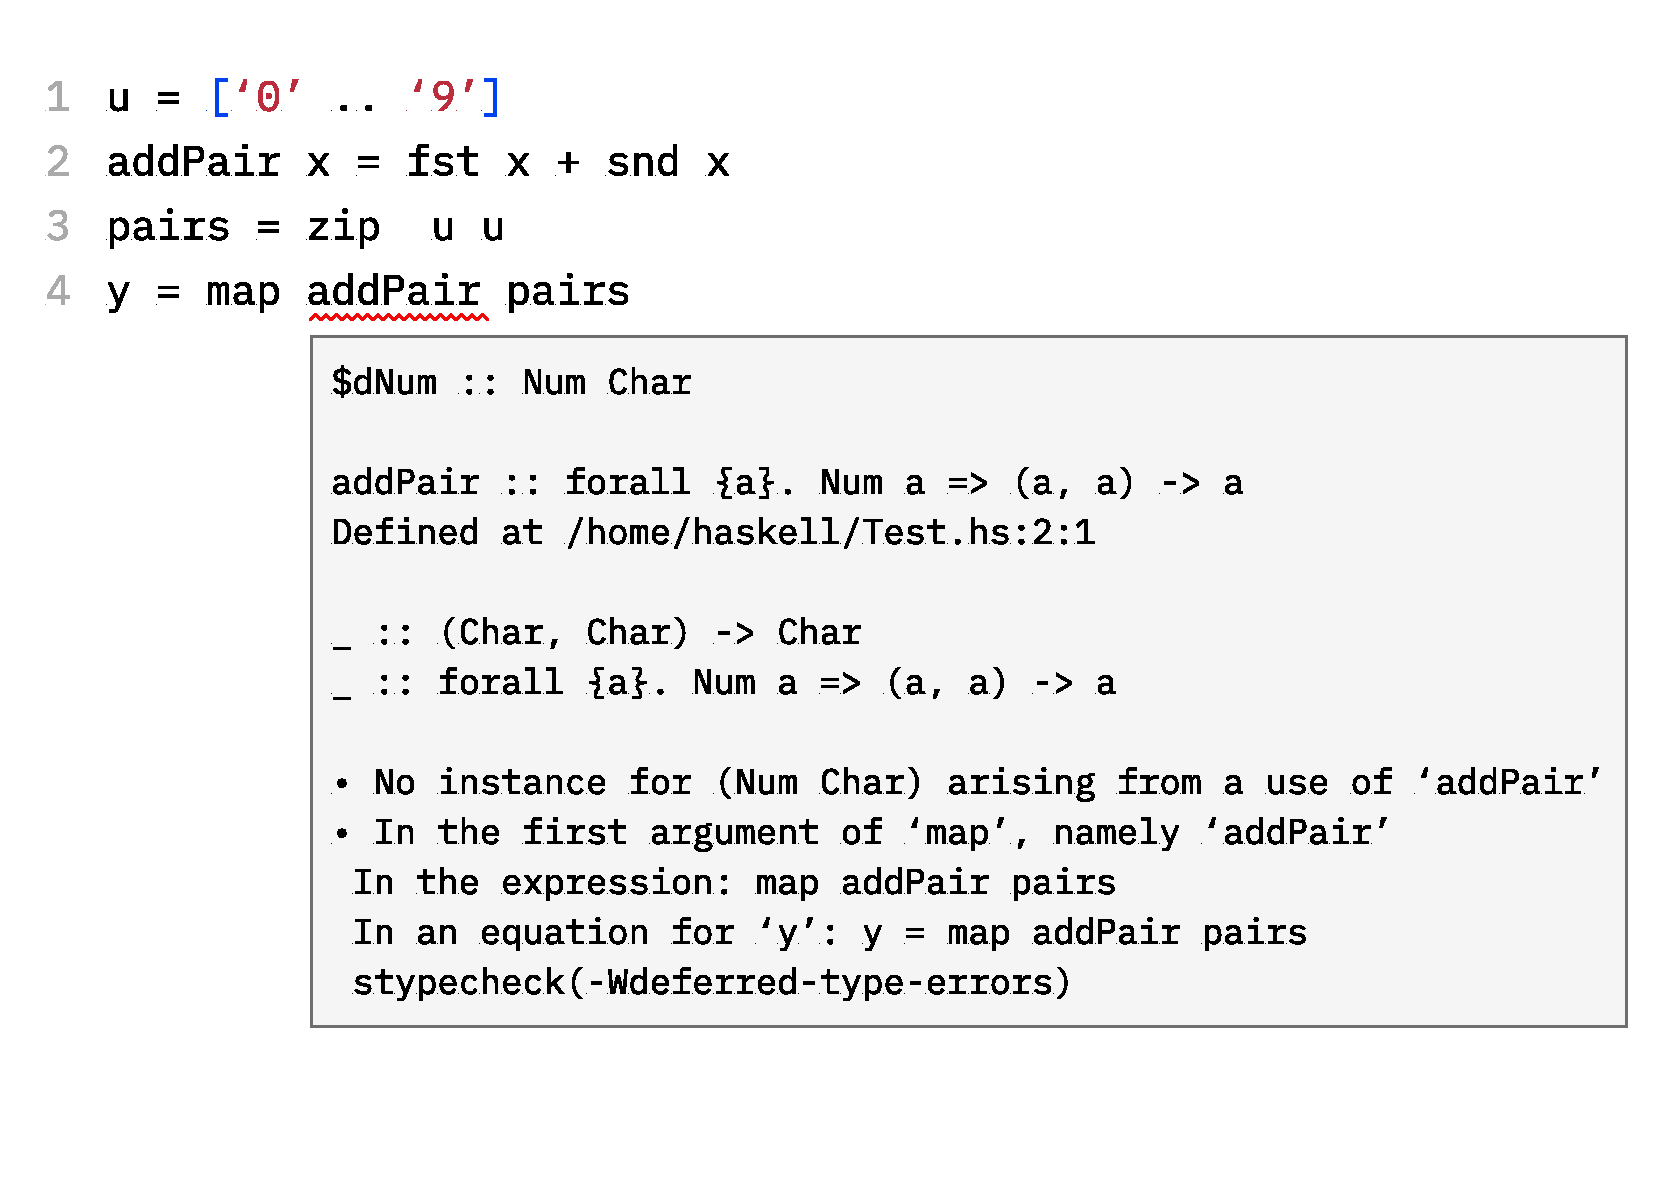
\includegraphics[width=\linewidth,trim=0mm 35mm 0mm 0mm]{images/add-pair-example.pdf}
    \caption{
    A type error displayed in Visual Studio Code\cite{microsoft_visual_nodate} and the Haskell Vscode extension\cite{haskell_haskell_nodate}.
The expression \texttt{addPair} is blamed for causing the type error. This may not match the programmers' intention. 
    }
    \label{fig:motivation-example}
\end{figure}
\subsubsection{\textbf{Traditional type errors show only limited location}}
Haack and Wells~\cite{haack_type_2004} noted that ``\textit{Identifying only one node or subtree of the program as the error location makes it difficult for programmers to understand type errors. To choose the correct place to fix a type error, the programmer must find all the other program points that participate in the error.}'' The type error in Fig.~\ref{fig:motivation-example} can be fixed in multiple locations. For instance  replacing \texttt{['0'..'9']} on line 1 with \texttt{[0..9]}, or replacing \texttt{fst x} and \texttt{snd x} on line 2 with \texttt {read (fst x)} and \texttt{read (snd  x)}. In the type error message, only the \texttt{addPair} expression on line 4 was blamed.  In this small example, the whole context is visible, but it can be more problematic in large programs where the lines contributing to the type error are far apart in the source code.

\subsubsection{\textbf{Traditional type errors are biased}}
A common form of bias happens when a type error is reported in one expression, but it can occur in multiple other expressions as well. In Fig.~\ref{fig:motivation-example}, the error message arbitrarily focuses on only \texttt{addPair}, while ignoring that the literals in the definition of \texttt{u} may be incorrect. %Technically, this results from the side effect of different unification orders of the internal type-checking technique and has no bearing on what the programmers think and expect. 
Another form of bias is that traditional type errors are often framed as conflicts between \texttt{Expected type} and \texttt{Actual type}. This framing is standard practice in most typed languages. However, what is the \texttt{expected} and what is \texttt{actual} are a side effect of different unification orders rather than the intention of the programmer. In both forms, the error message may lead programmers to falsely believe the validity of parts of code and wrongly accuse others.

\subsubsection{\textbf{Traditional type errors give poor explanations}}
When the compiler rejects a program, the internal state of type checking is the result of a complex computation. But the details of this process are hard to explain to users and are usually not reported by compilers. For the typical type error shown in Fig.~\ref{fig:motivation-example}, the evidence for the type error is gathered from the previous two declarations. These have to be rediscovered by programmers using less rigorous methods. 

\subsection{Design Goals of \chameleon{}}
Based on the limitations of traditional type errors, we give the following design requirements for \chameleon{}:

\noindent\textbf{Show} all the possible locations where the type error happened or could have happened.

\noindent\textbf{Explain} type errors avoiding jargon and internal constructs of the type checker.

\noindent\textbf{Do not presume} which expression is to blame for the type error based on the order of computation or which possible type for an expression is 'actual' or 'expected'.


\section{Chameleon IDE} \label{chameleon}
\begin{figure*}
    \centering
    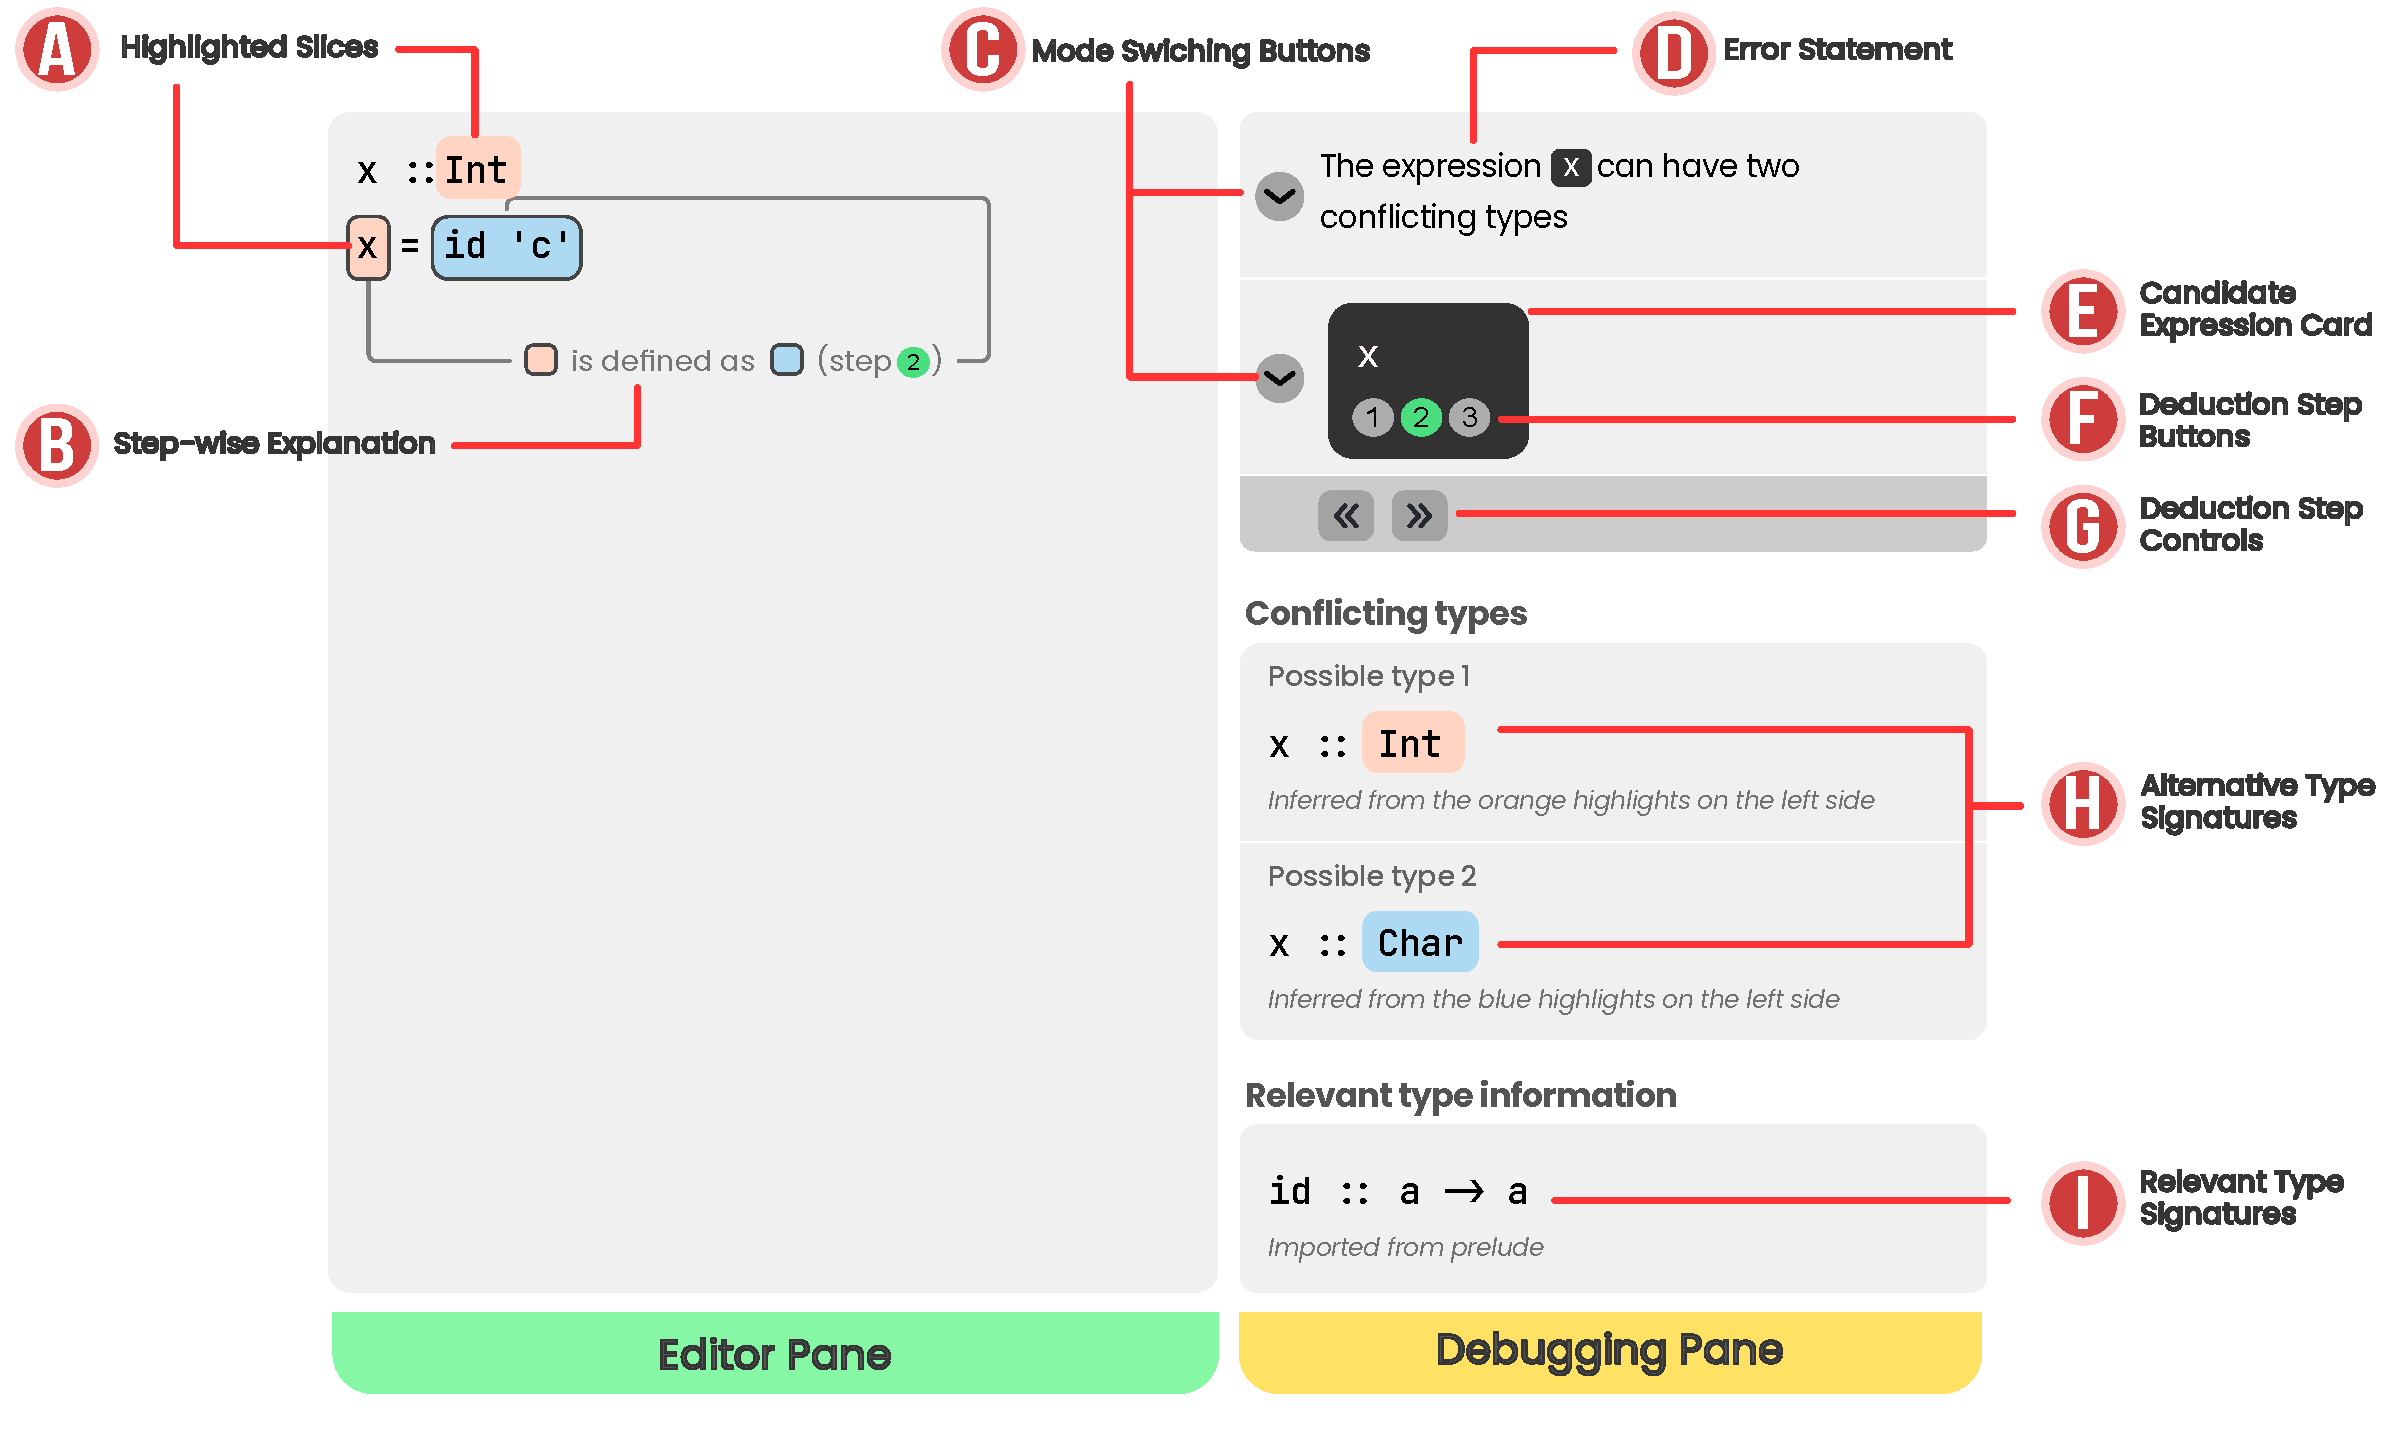
\includegraphics[width=\textwidth, trim=0mm 10mm 0mm 0mm]{images/atonomy.pdf}
    \caption{
        \textbf{The anatomy of \chameleon{}.}
        The editor pane (left) is similar to a traditional code editor. Fragments of source code may have a highlight
        color (A). Additionally, an explanation layer (B) displays if deduction steps are enabled. The debugging pane contains three blocks. First, the error statement block contains an error statement (D), optionally, a list of candidate expression cards (E), a list of deduction steps (F), and a control bar (G) to increment/decrement deduction step. Second, the conflicting types block shows two alternative types (H). Third, the relevant type information block shows additional information (I) that may help understand type errors.
    }
    \label{fig:anatomy}
\end{figure*}


\chameleon{} comprises two parts: a type inference engine and a novel interactive debugging interface. This separation of concerns allows us to (1) adapt \chameleon{} into multiple front ends, such as IDE extensions, desktop applications, and web applications; and (2) reuse the debugging interface for different programming languages by replacing the back-end type inference engine. The debugging interface is designed from the ground up; the type inference engine is a re-implementation of the original Chameleon with several novel improvements, as described in Section \ref{sec:typeinferenceengine}.

\todo{I wonder about a high level overview diagram of tool / usage of tool, then the details of each component?}

\todo{Can you use this example in Motivating Example sectoon (see my comment above) then use it to explain tool in this section?  Make sense?

Is this example too simple...?}

\subsection{The Debugging Interface}

The \chameleon{} debugging interface provides three main features to visualize the relation between the error statement and locations in code and to explore the explanation of each error location given by the type inference engine. %Further, programmers  can turn on and off features to suit their preferences and debugging needs.


\paragraph{Type compare tool} \label{sub:type-compare}
% In designing \chameleon{}, we want to argue against the practice of reporting type errors as the conflicts between \texttt{Expected type} and \texttt{Actual type}. Technically, the two alternatives are merely the side effect of different unification orders of the internal type-checking technique and have no bearing on what the programmers think and expect. 

The type compare tool shows conflicting types in different colors, each type associated with one or more error locations highlighted in a matching color (Fig.~\ref{fig:compare}).  
%The type error must be fixed by modifying at least one of these locations. 
%Error locations are highlighted with the matching color of the conflicting types. The type compare tool is useful to quickly bisect the type error. 
If the programmers know the expression's intended type (they usually do), they will be able to eliminate half of the possible locations. 
%To make this bisecting effect more pronounced, a user can hover over one of the possible types and only show the relevant locations that contribute to that type. 
A hover interaction over one of the possible types facilitates such bisection, causing only the relevant locations that contribute to that type to be highlighted. 
%This is a convenient way to put the error \emph{under the spotlight}.


\begin{figure}
    \centering
    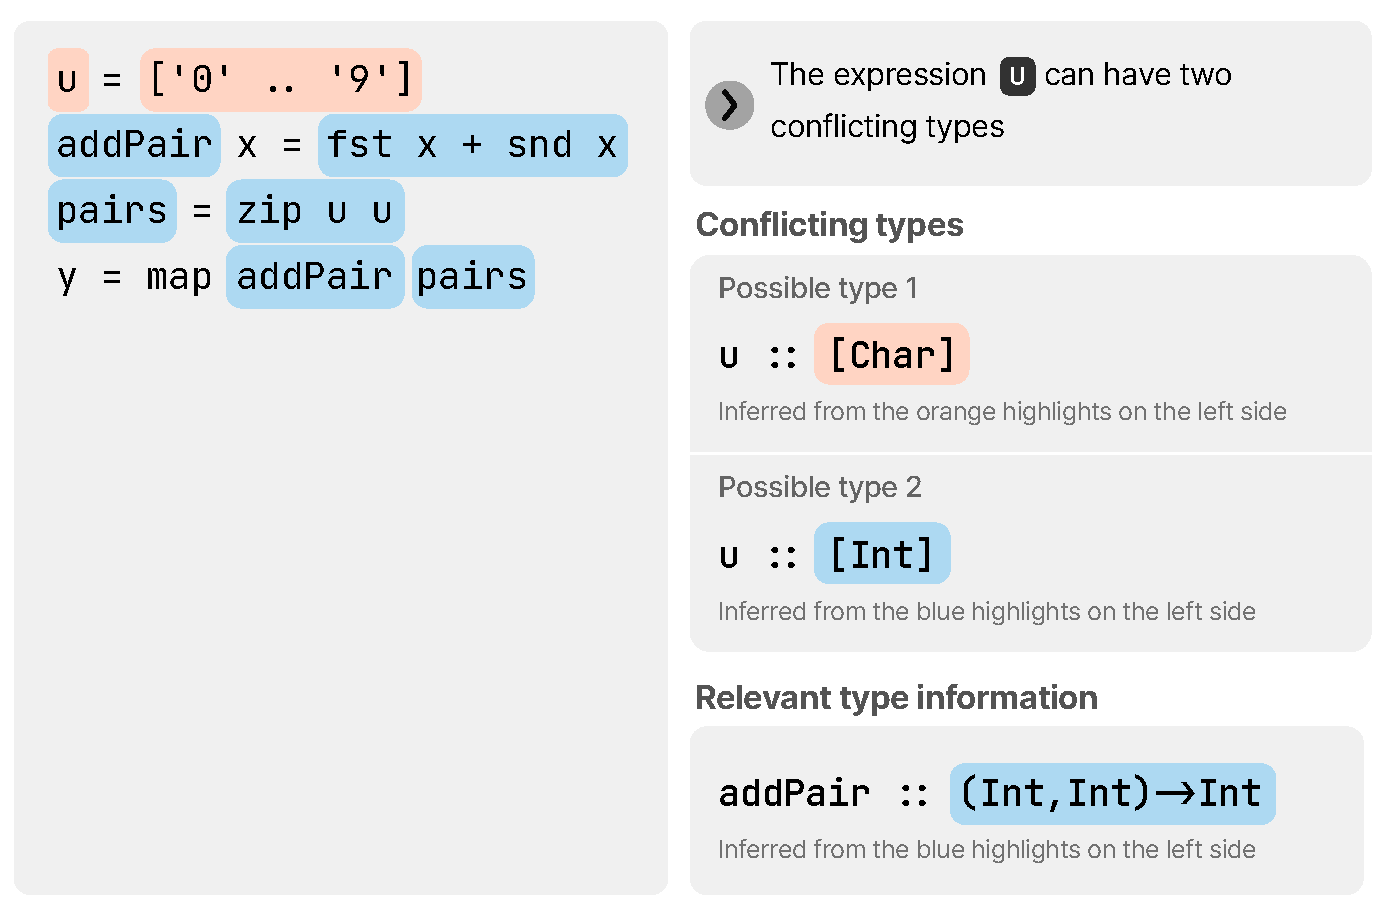
\includegraphics[width=\linewidth, trim=0mm 10mm 0mm 0mm]{images/intro-compare-2.pdf}
    \caption{
        \textbf{\chameleon{} with type compare tool enabled}. \chameleon{} identified the conflicting types for the expression \texttt{u} and associated the relevant locations with each type. Compare the output with the traditional type error message in fig. \ref{fig:motivation-example}.
}
    \label{fig:compare}
\end{figure}

\begin{figure}
    \centering
    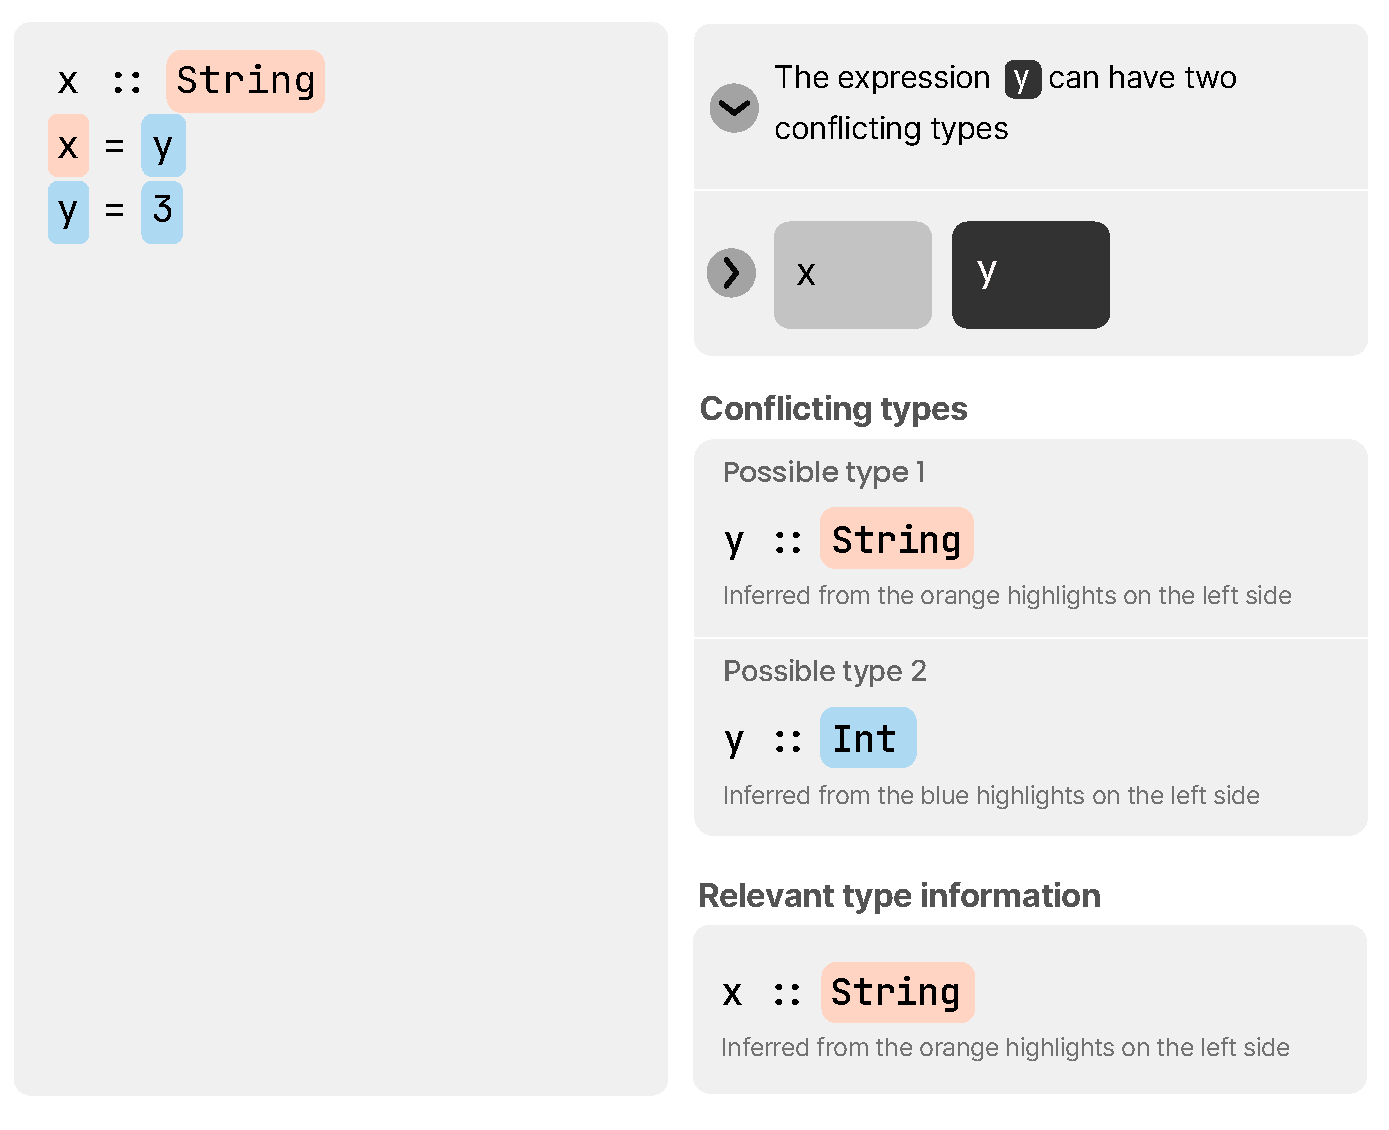
\includegraphics[width=\linewidth, trim=0mm 10mm 0mm 0mm]{images/intro-candidate.pdf}
    \caption{
        \textbf{\chameleon{} with candidate expression cards enabled.}
        Indicates the type error can occur in the definition of \texttt{x} or \texttt{y}.
    }
    \label{fig:expression}
\end{figure}


\begin{figure}
    \centering
    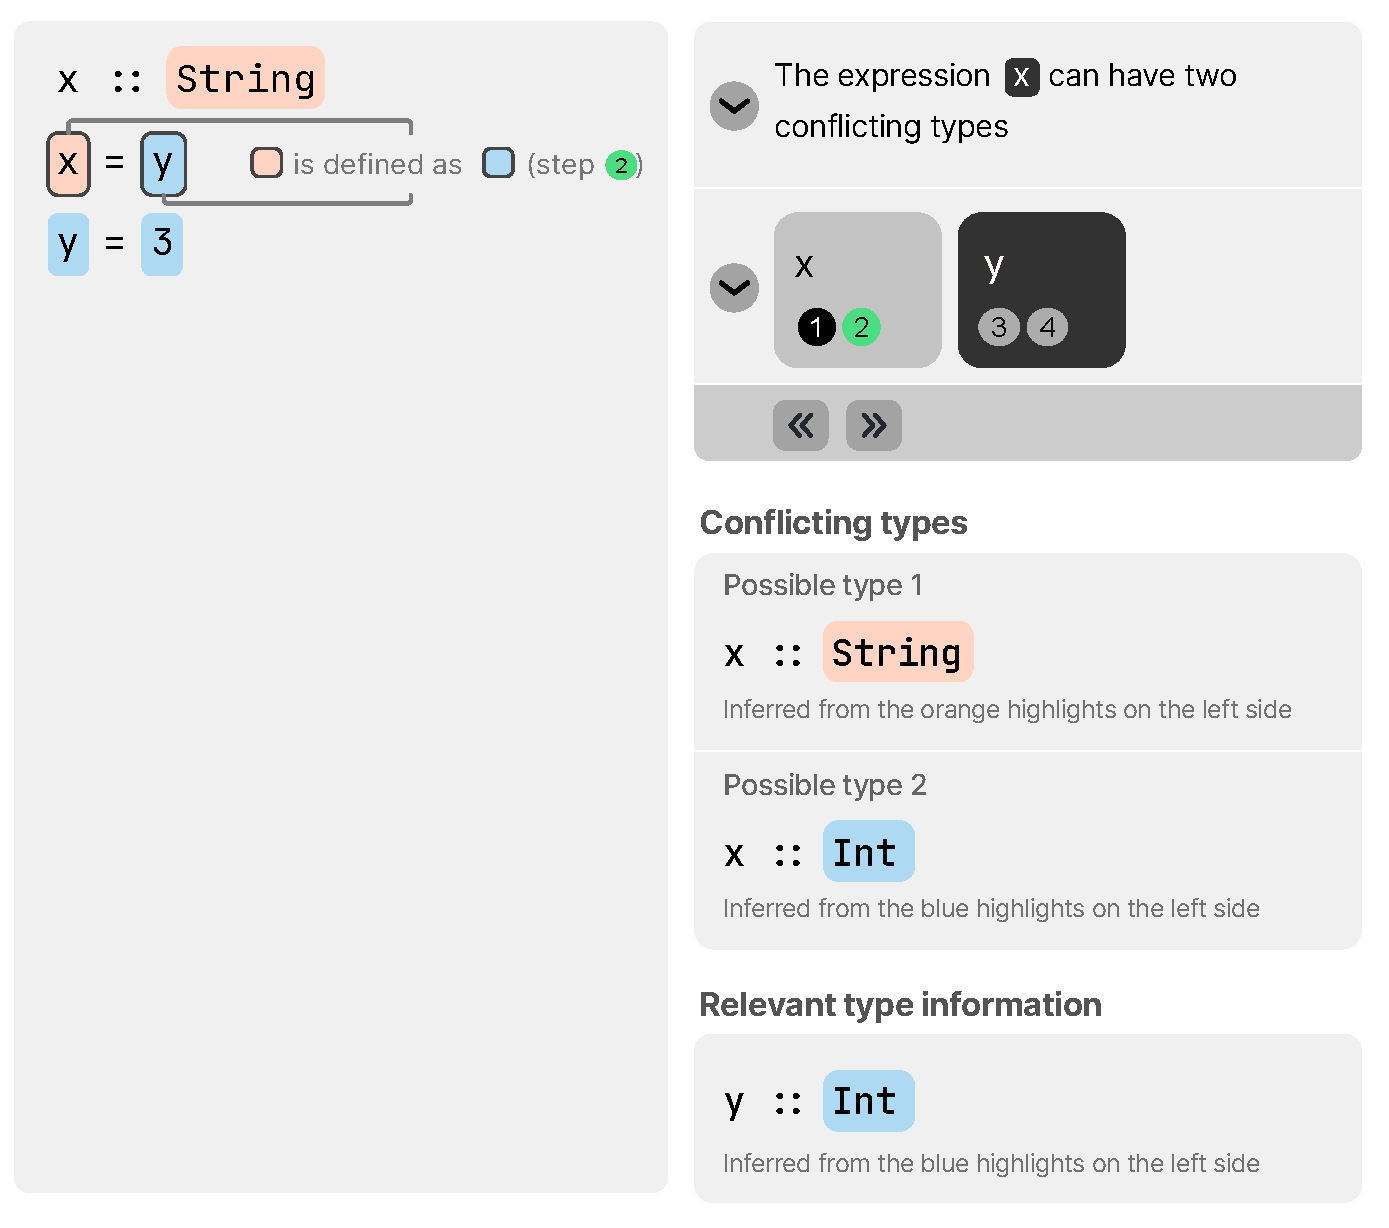
\includegraphics[width=\linewidth, trim=0mm 10mm 0mm 0mm]{images/intro-deduction.pdf}
    \caption{
        \textbf{\chameleon{} with deduction steps enabled.}
        \chameleon{} explains the type error in four steps. In the screenshot, the active step is step 2, where \chameleon{} shows that the expression \texttt{x} and \texttt{y} should have the same type. 
    }
    \label{fig:deduction}
\end{figure}



\paragraph{Candidate Expression Cards}  \label{sub:candidate-expression}


% We propose candidate expression cards to make it clear to the user that there are multiple ways to resolve a type conflict. By contrast,  standard compiler error messages such as those of GHC arbitrarily focus the users' attention on only one candidate expression, e.g.\ ``\textit{Couldn't match expected type ‘Char’ with actual type ‘Bool’ in expression x}" where x is the candidate expression. In practice, this candidate expression often does not match programmers' intention (Fig. \ref{fig:single-candidate}).  
A candidate expression is an expression that can be inferred to have two conflicting types. 
When a type error is detected, \chameleon{} provides a list of all candidate expressions, and programmers are free to choose the problem to resolve by clicking on one candidate expression card. In the example shown in Fig. \ref{fig:expression}, \texttt{x} and \texttt{y} are both candidate expressions. Fixing either type error can make both expressions well-typed.


% This feature can be effective in resolving the problem that traditional tools tend to report errors that happened in source code from third-party libraries. With candidate expression cards, a programmer can freely change the context of the type error to the user-defined variables and functions to gain a better understanding of why their own code does not match the library code instead of the other direction.


Programmers select a candidate expression card by clicking on one card. Once a card is selected, the information in the conflicting types block changes to reflect the change of candidate expression. In the editor pane, some error locations change highlight colors based on the updated candidate expression. Alternatively, programmers can preview the change of a candidate expression by hovering on one card. The hover effect is reverted once the cursor moves away. 


\paragraph{Deduction steps}  \label{sub:deduction-steps}

% Deduction steps are motivated by the lack of explaining why the program has type errors. When the compiler rejects a program, it dumps the internal state of type checking.  This information may be a result of complex computing but this process is not reported by compilers. For a typical type error shown in Fig. \ref{fig:ghc-error-example}, clearly, the evidence for the type error is gathered from the previous two declarations. These have to be rediscovered by the programmers again, using harder and less-sound methods. 

% \begin{figure}
%     \centering
%     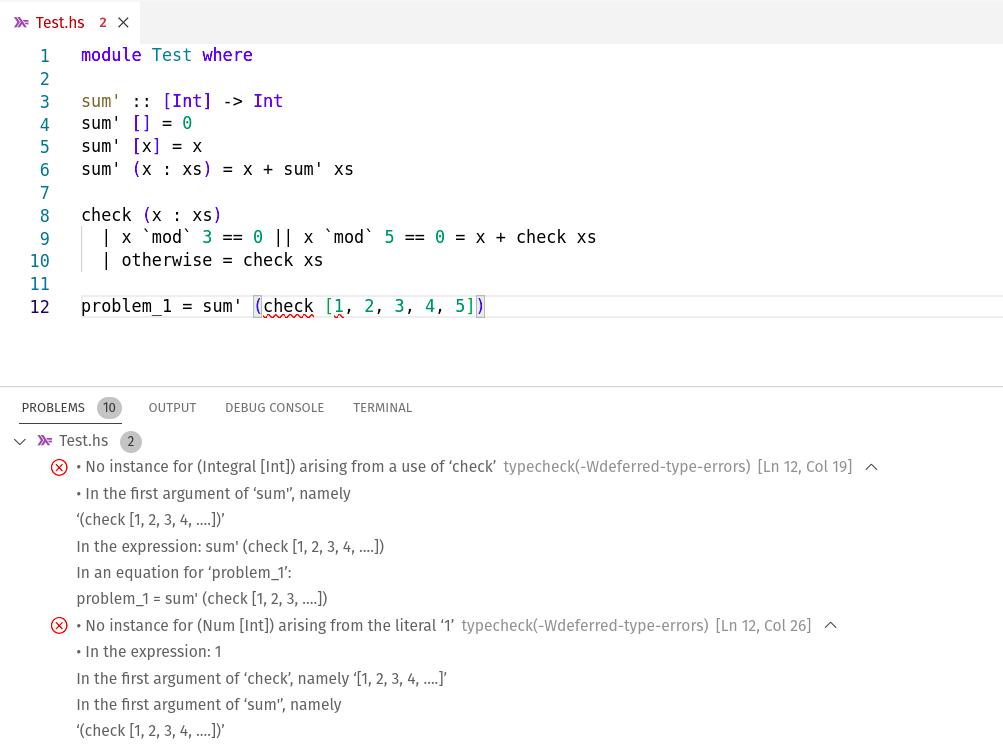
\includegraphics[width=\linewidth]{images/ghc-error-example.png}
%     \caption{
%         }
%     \label{fig:ghc-error-example}
% \end{figure}

Deduction steps allow programmers to explore all the error locations one at a time (Fig. \ref{fig:deduction}). Steps are shown as a list of sequentially  numbered circular buttons (step buttons) and an explanation layer in the editor window. In the explanation layer, the two locations under examination are outlined, and a line is drawn to connect these two locations. This line is accompanied by a human-readable text explanation of their semantic connection. Programmers are free to activate any step. The active step is shown in green. When activating a step, some highlights switch color. The message in the explanation layer changes as well. A program in Fig. \ref{fig:deduction} generates a list of steps shown in Fig. \ref{fig:step-interface} left.


Programmers can use mouse and keyboard shortcuts to increment or decrement the step number or jump to any step. Programmers resolve type errors by navigating through all the deduction steps and verifying whether each explanation aligns with their intention. Eventually, they will find a step that does not match, and the type error can be fixed by modifying one of the two outlined locations.

\begin{figure}
    \centering
    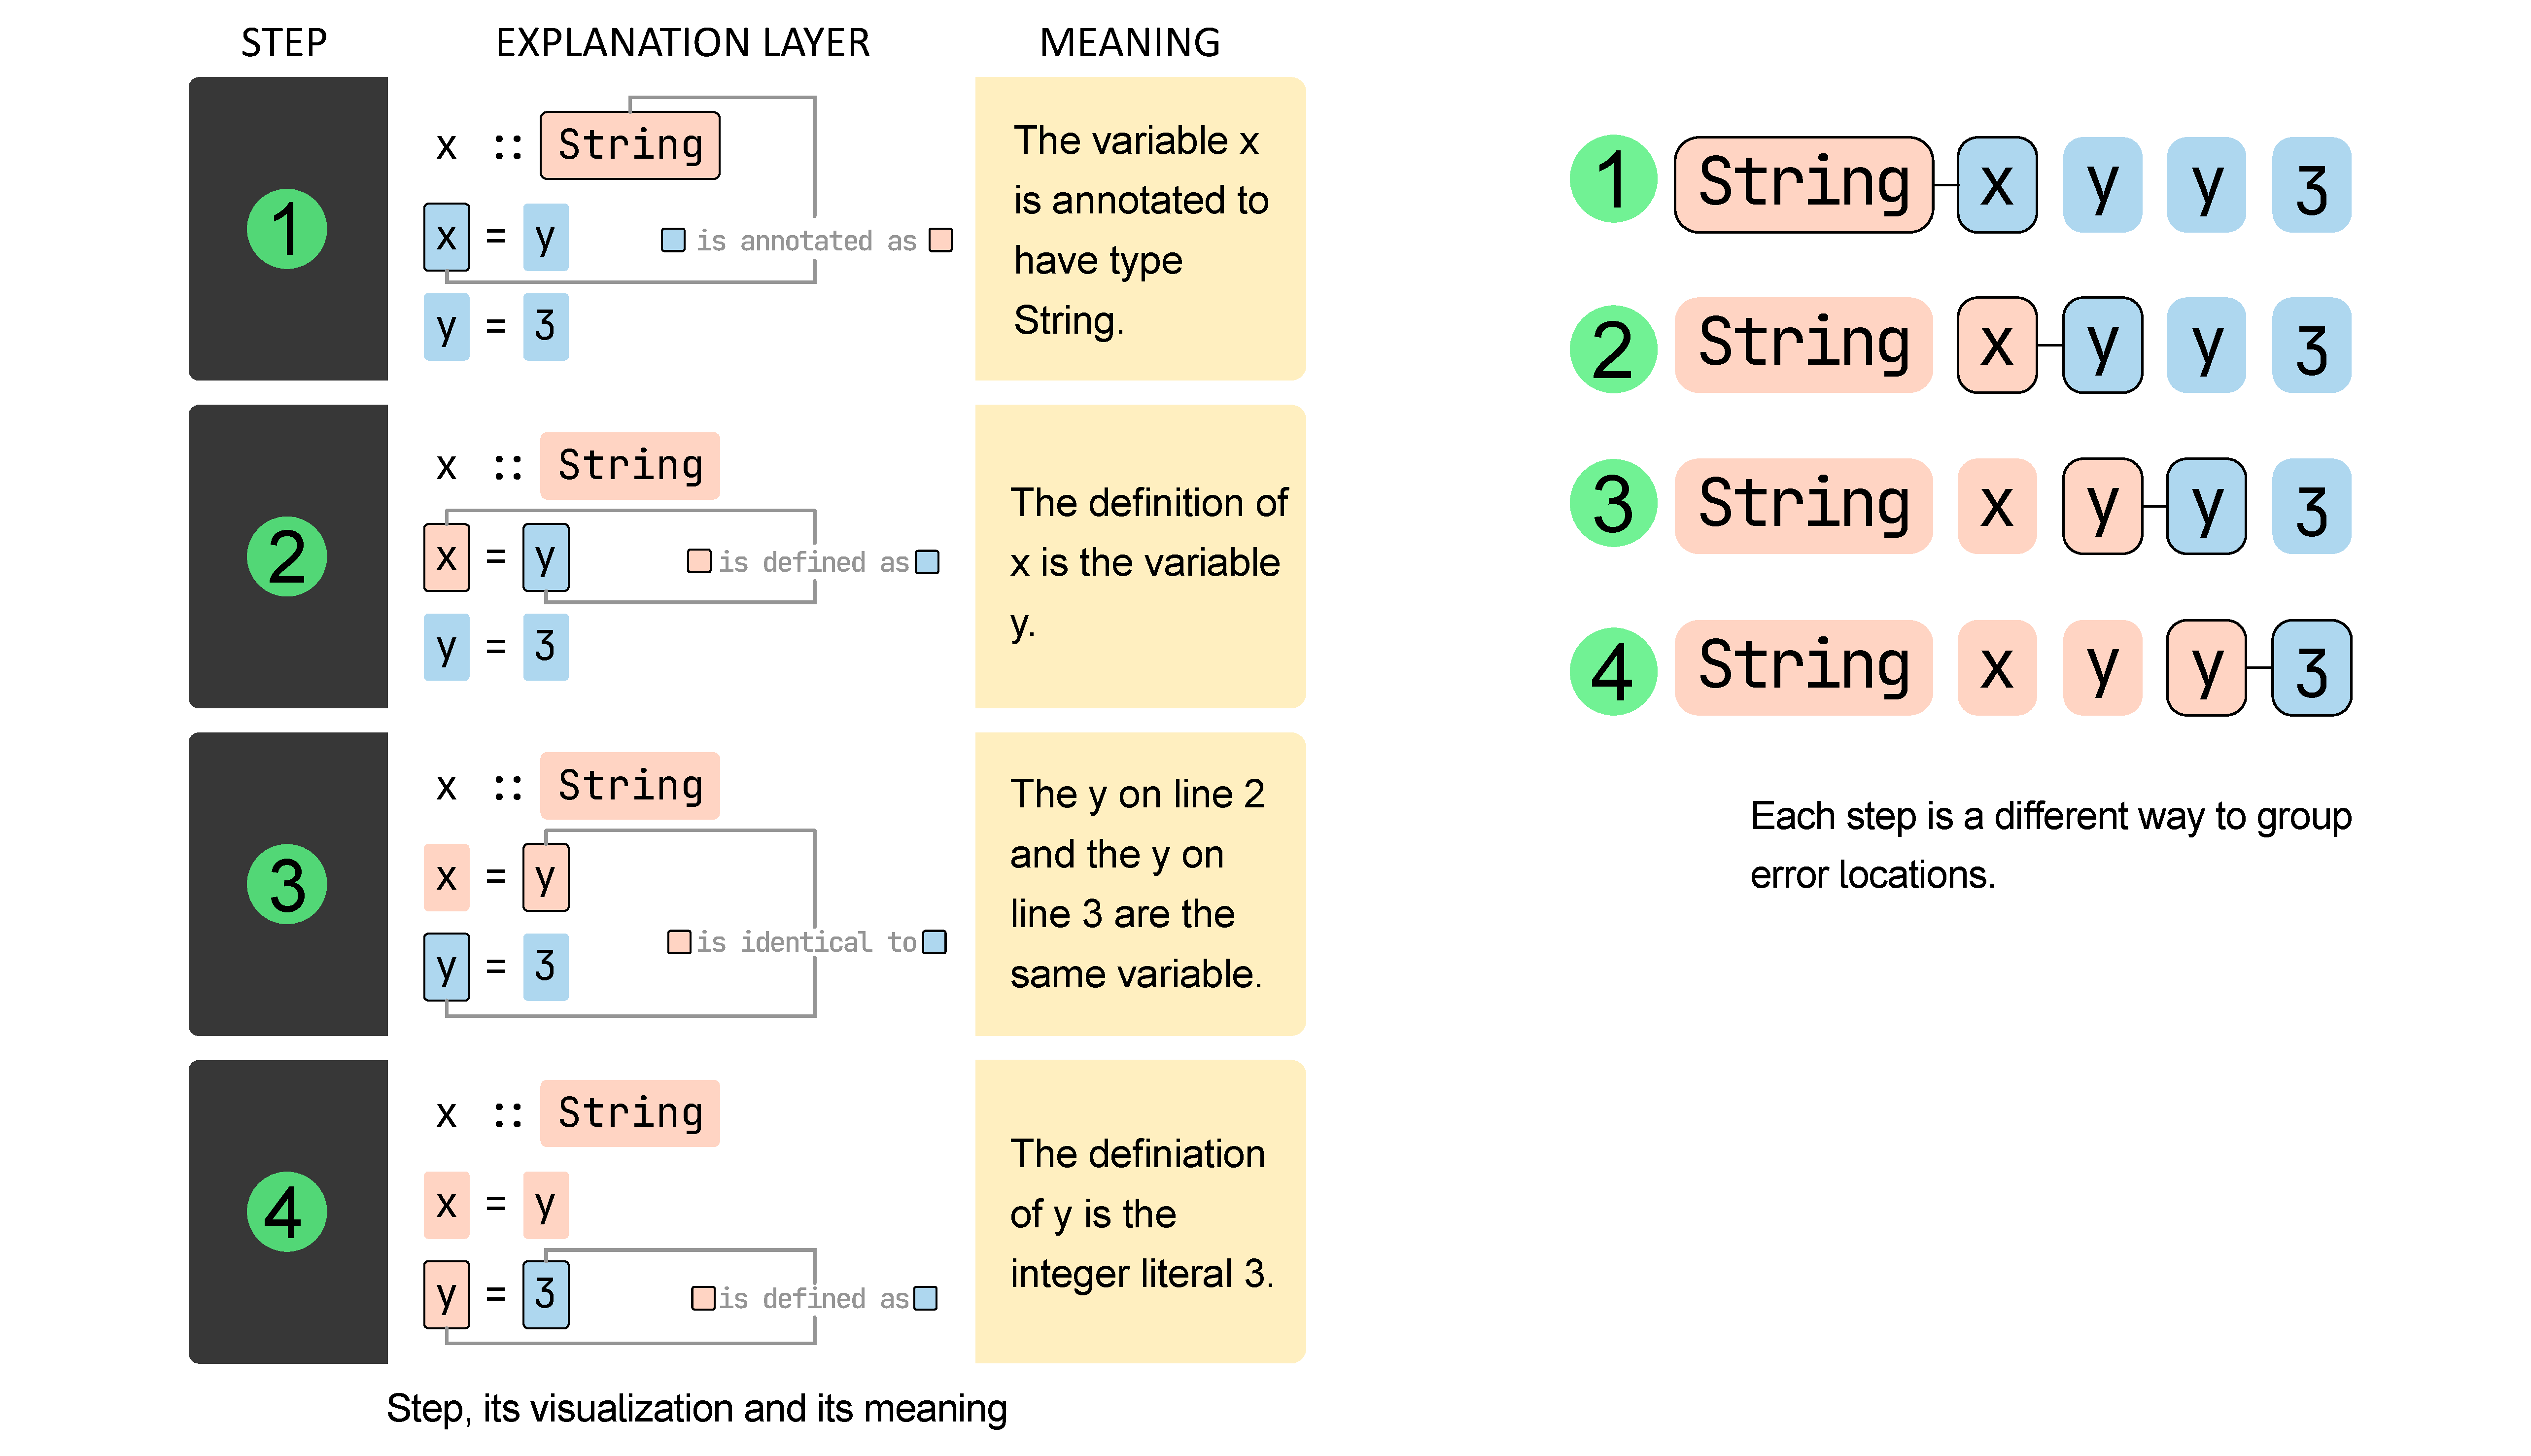
\includegraphics[width=\linewidth, trim=0mm 10mm 0mm 0mm]{images/step-interface.pdf}
    \caption{
Deduction steps if they are shown all at once (left). In practice, steps are shown one at a time. Programmers increment or decrement the step number using the step control bar (Fig. \ref{fig:anatomy}-G) or by directly clicking on a step button (Fig. \ref{fig:anatomy}-F). To increment or decrement the deduction step can be intuitively thought of as moving the position of the \textit{split point} where the blue and orange highlights divide (right).
        }
    \label{fig:step-interface}
\end{figure}

Internally, deduction steps are different ways to group the error locations into two highlighted colors. All the relevant constraints (highlights) are divided into two groups, denoted by the two colors. Each color infers a different type of the candidate expression. Each increment of the step changes the place where the two colors are divided by moving one constraint from one color to the other.  (Fig.~\ref{fig:step-interface} right).


\paragraph{Multiple Modes}

Nielson pointed out  that the two most important issues in designing for usability are understanding the users' tasks and the differences in users \cite{jakob_nielsen_usability_1993}. From analyzing how users use \chameleon{}, we realized that the ideal debugging interface should adapt to the specific programmer and programming task. There are cases where a programmer wants the debugger to simply ``show the answer", and others to dive deeper into the problem domain and search for the optimal solution. To accommodate the need to customize the level of information density and granularity of control, \chameleon{} provides three modes: basic, balanced, and advanced. Programmers can switch between modes by clicking on the mode switching toggles (Fig. \ref{fig:anatomy}-C). The features accessible from different modes are summarised in the following table:%shown in table~\ref{tab:chameleon-features}.

% \begin{table}
%     \centering
\begin{scriptsize}
\begin{center}
    \begin{tabular}{ l l  }
     \textit{Mode} & \textit{Features} \\ \hline
     Basic Mode & Type Compare Tool \\ \hline
     Balanced mode & Type Compare Tool \\
     & Candidate Expression Card \\  \hline
     Advanced mode & Type Compare Tool \\
     & Candidate Expression Card \\
     & Deduction Steps \\
    \end{tabular}
    \end{center}
\end{scriptsize}
%     \caption{\chameleon{} modes and features}
%     \label {tab:chameleon-features}
% \end{table}


\subsection{The Type Inference Engine}
\label{sec:typeinferenceengine}

Chameleon was originally a command-line tool developed in the early 2000s to improve type error reporting %and introduced a design for interactive type debugging 
for the Haskell programming language.
Unlike traditional type errors produced by the Glasgow Haskell Compiler (GHC)~\cite{ben_gamari_home_2022}, which uses a Hindley–Milner type inference system, Chameleon infers types using constraint solving. In Chameleon, constraints are generated from the source code based on typing rules. In addition, each constraint is labeled with the location where it is generated. This set of constraints is consistent if the program is well-typed and inconsistent otherwise. When a type error occurs, an efficient algorithm is used to derive a minimal subset of the constraints that still contain inconsistencies. This subset is called a Minimal Unsatisfiable Subset (MUS). From this, Chameleon can report a list of locations, using the labels of constraints that are in the MUS. Stuckey et al.~\cite{stuckey_interactive_2003} showed that program locations linked to the constraints from an MUS are all relevant to the type error and must include the cause of the error.

Despite successfully borrowing the underlying ideas, we could not reuse the original implementation of Chameleon since the project language standard and libraries used were out of date. 
Our \chameleon{} implementation extends the original Chameleon approach in a number of ways.
%In addition to what Chameleon can do, a few new type inference features were added in the \chameleon{} implementation.



\paragraph{Recovering concrete types from type errors}


Using only constraints from the MUS is sufficient to locate the type error, but to recover types from type errors we need  constraints from parts of the program that are irrelevant to the type error.  For instance, consider an ill-typed 2-tuple where two possible types can be assigned: \texttt{(Int, Int)} and \texttt{(Int, String)}. The types reconstructed from Chameleon may be \texttt{(a, Int)} and \texttt{(a, String)}. Although the recovered types are theoretically correct, they introduce a new type variable \texttt{a}, making the error message harder to understand. To solve this issue in \chameleon{}, for each constraint \texttt{c} in the MUS, we find a maximally satisfiable subset (MSS) from all the constraints that contain every other element of MUS but not \texttt{c}. These maximally satisfiable subsets, while not helpful to inform error locations, will produce the most concrete conflicting types, see Fig.~\ref{fig:compare-to-original}. 


\begin{figure}
    \centering
    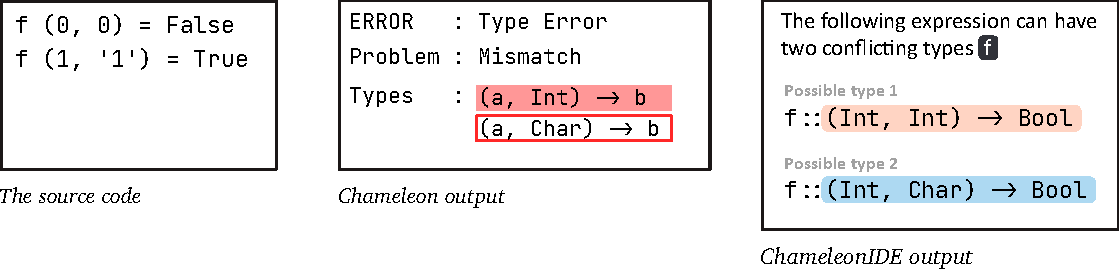
\includegraphics[width=\linewidth, trim=0mm 6mm 0mm 0mm]{images/compare-to-original.pdf}
    \caption{
Reporting the same type error, Chameleon uses
\texttt{Int -> a} and \texttt{Char -> a}, while \chameleon{} uses the 
concrete types \texttt{Int -> Bool} and \texttt{Char -> Bool}.
    }
    \label{fig:compare-to-original}
\end{figure}

Using concrete types provides extra information to programmers. With a type of \texttt{(Float, Float)}, programmers may want to convey a point in 2d space. However, a type of \texttt{(a, Float)} does not preserve such information. If the types get too verbose for programmers to identify the conflict between the two signatures, it is always possible to mute the overlapping information and highlight the differences from the debugging front end.


\paragraph{Type error explanation}

In addition, \chameleon{} provides support for type explanation. Similar to the type explanation system  in ~\cite{jun_explaining_2002},  \chameleon{} is able to produce a human-readable explanation, but for type errors. This is achieved by annotating nodes in the abstract syntax tree with constraints and the typing rules used. We generate an inference history from constraints and accompanying annotations. 


% \begin{lstlisting} [
%     language=Haskell, caption={
%     A simple program that is ill-typed. This program generates two constraints from line 1 and one constraint from line 2.
% }, label={listing:ifelse}
% ]
% if a then b else c
% a = "True"
% \end{lstlisting}
\begin{listing}[!ht]
\begin{minted}{haskell}
    if a then b else c
    a = "True"
\end{minted}
\vspace{-3mm}
\caption{A simple program that is ill-typed. It generates two constraints from line 1 and one constraint from line 2. }
\label{listing:1}
\end{listing}
For instance, for the program in Listing~\ref{listing:1}, \chameleon{}  generates the following constraints and labels (in brackets) $T_a = Bool$ (if condition), $T_b = T_c$ (if branches), $T_a= String$  (definition). Clearly, as $T_a$ can not unify with both \textit{Bool} and \textit{String}, this program is not well typed. \chameleon{} can construct a human-readable explanation from the MUS. An example output for Listing~\ref{listing:1} can be: \texttt{a} has type \texttt{Bool} because \texttt{a} is the condition of an if statement; however, \texttt{a} has type \texttt{String} because \texttt{a} is defined as the string literal \texttt{"True"}. This explanation facilitates the deduction steps (Section \ref{sub:deduction-steps}).







\section{Walkthrough} \label{sec:walkthrough}
In this section, we introduce \chameleon{} by walking through examples of its
use. The examples are given from the perspective of a hypothetical Haskell 
programmer Maxine. 


\subsection{Basic mode} \label{sub:basic}
Maxine writes a function to calculate the sum of a list of
numbers, but \chameleon{} shows there is a type error (Fig. \ref{fig:basic-mode-1}). 
After reading error reports, Maxine realized that the error possibly revolves 
around the expression \texttt{xs}.

\begin{figure}[h]
        \centering
        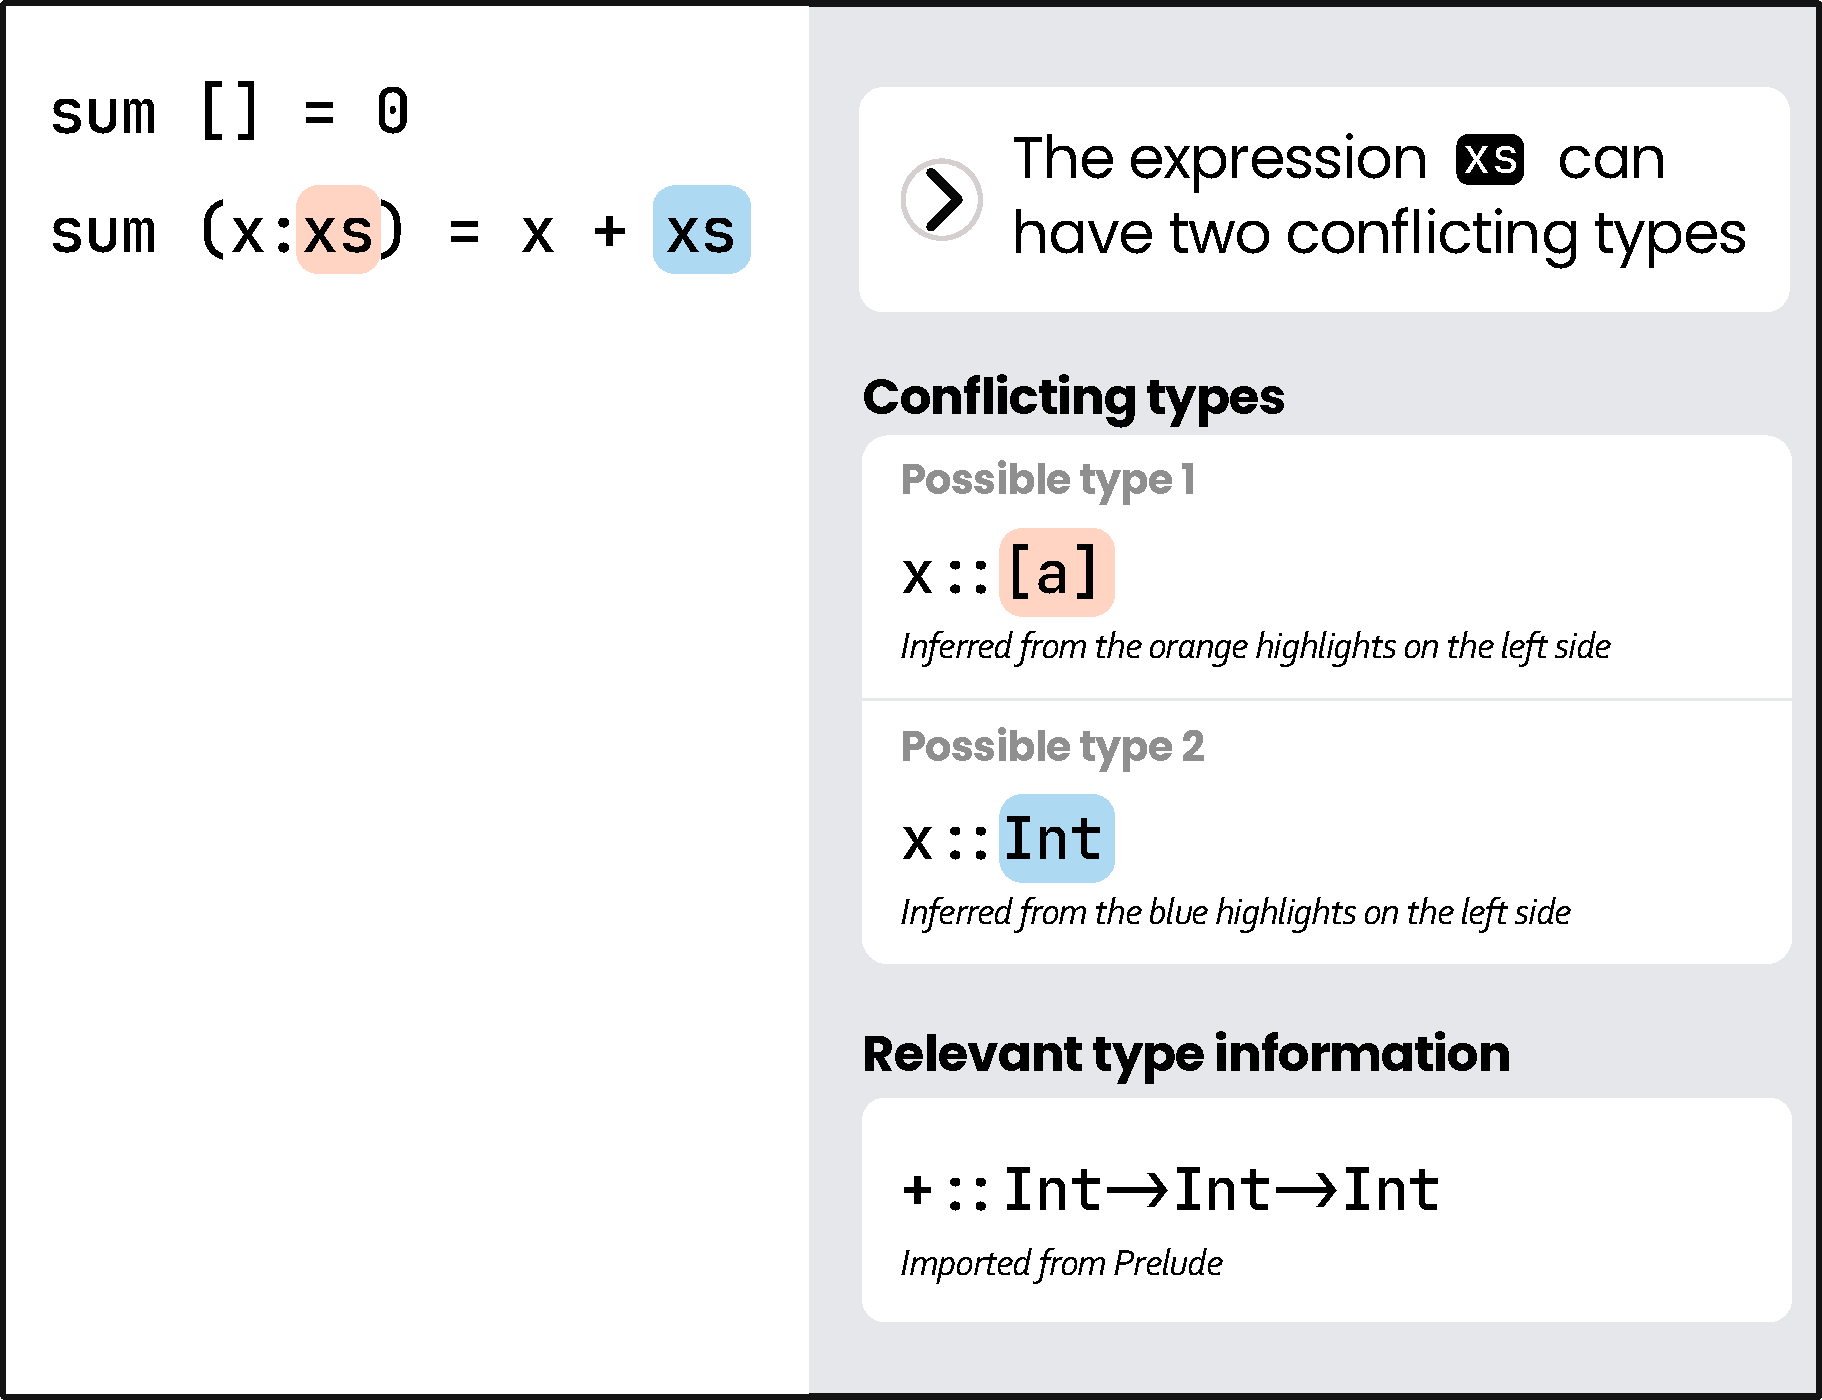
\includegraphics[width=\linewidth]{images/basic-mode-1.pdf}
        \caption{
            Maxine's code to calculate the sum of a list of integers;
            \chameleon{} reports an error on the expression \texttt{xs}.
            }
            \label{fig:basic-mode-1}
\end{figure}

\begin{figure}[h]
        \centering
        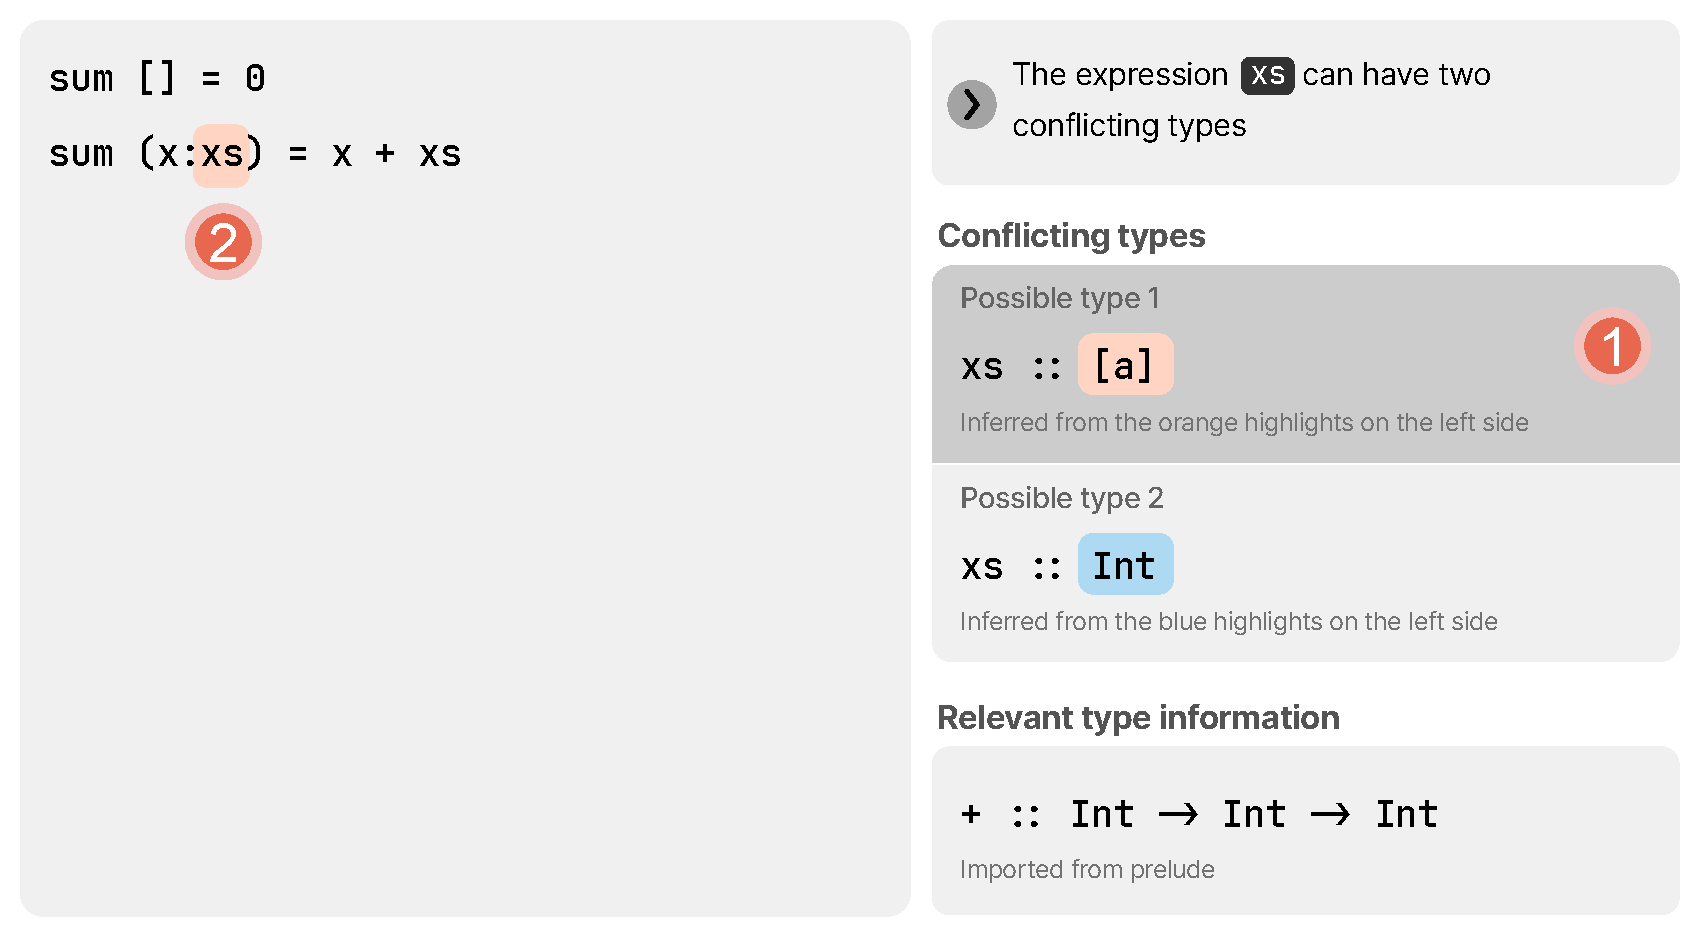
\includegraphics[width=\linewidth]{images/basic-mode-2.pdf}
        \caption{
       Hovering on possible type 1 will limit the highlights 
       in the editor to only the ones (in orange) that support \texttt{x::[a]}.
        }
        \label{fig:basic-mode-2}
\end{figure}

\begin{figure}
        \centering
        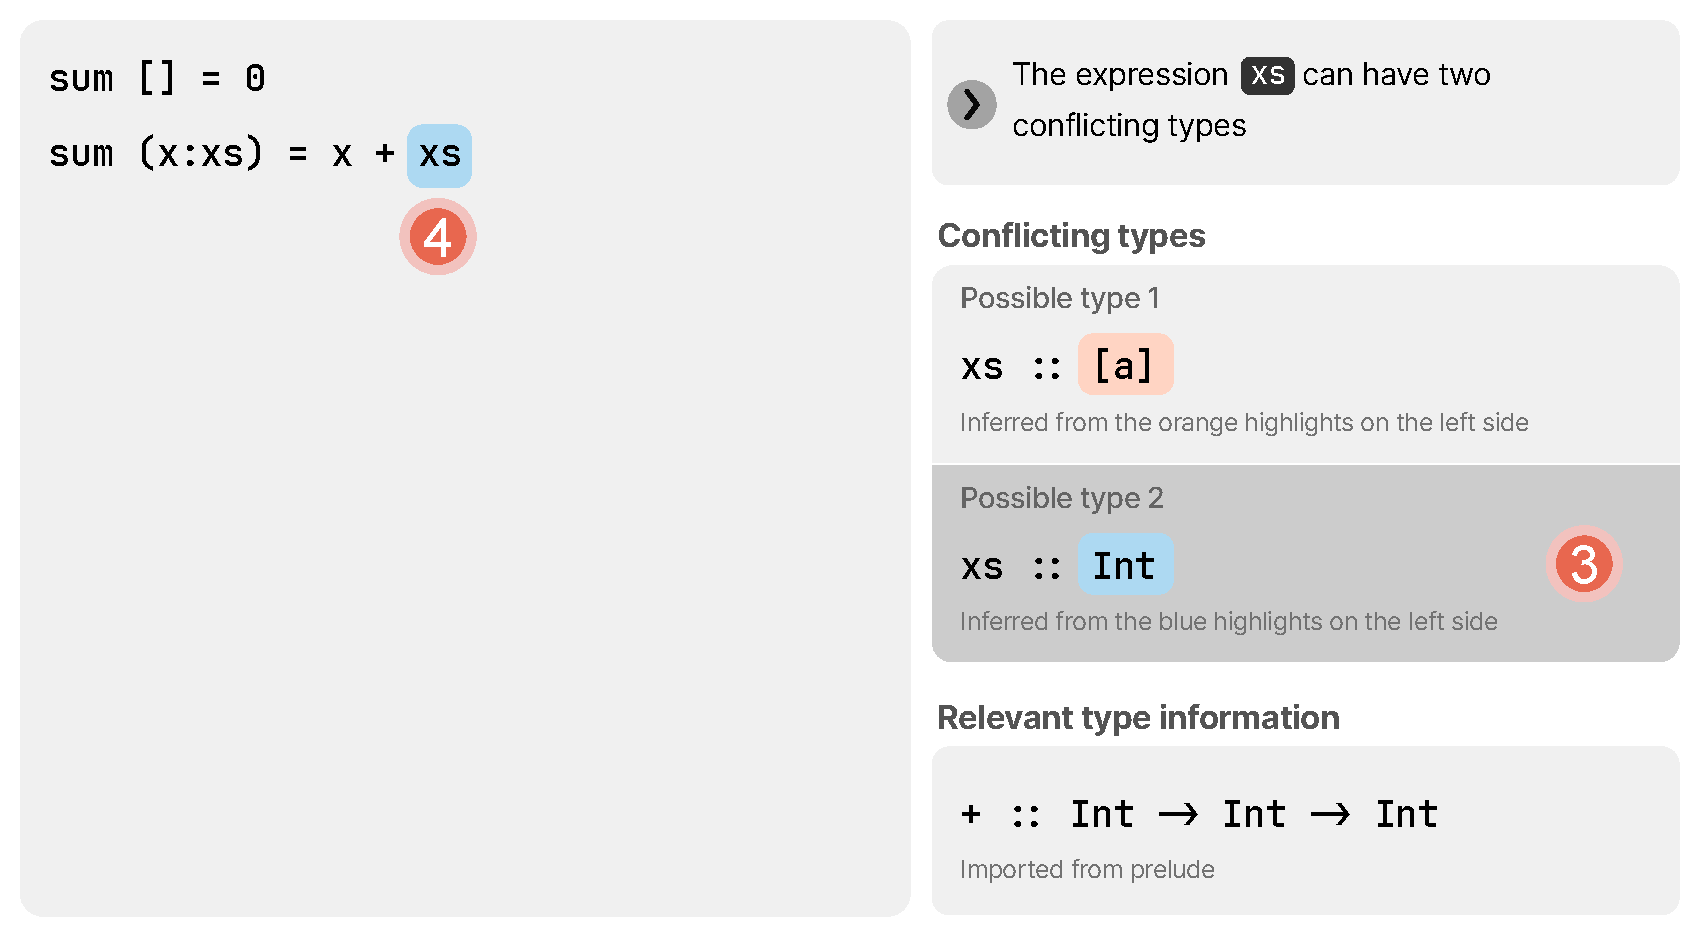
\includegraphics[width=\linewidth]{images/basic-mode-3.pdf}
        \caption{
            Hovering on possible type 2 (Fig. \ref{fig:basic-mode-2}-3) will limit the highlights 
            in the editor to only the ones (in blue) that support \texttt{x::Int}.
        }
        \label{fig:basic-mode-3}
\end{figure}





After scanning the type error report, Maxine realizes that \texttt{xs} can be
either \texttt{[a]} type (Fig. \ref{fig:basic-mode-2}) or \texttt{Int} type (Fig. \ref{fig:basic-mode-2}). By matching the color in the
conflicting type panel (Fig. \ref{fig:anatomy}-G) and the highlighted error locations 
Maxine knows that the \texttt{[a]} type results from the pattern matching of the
\texttt{:} operator, and the \texttt{Int} type results from using \texttt{+} to
 add two expressions. 


At this point, Maxine knows the possible type 1 aligns with her understanding of
the program, and therefore, the error locations with blue highlights must be
erroneous. After examining the program, it is obvious that Maxine missed
applying the \texttt{sum} function recursively at the right-hand side of the
addition. 


\subsection{Balanced mode} \label{sub:balanced}


Maxine writes additional code to add only the even numbers in a list of integers.
In this implementation, Maxine reuses the \texttt{sum} function she wrote
earlier. After saving the file, \chameleon{} shows that there is a type error in the
expression \texttt{sum} (Fig. \ref{fig:balance-mode-1}). However, this is not 
helpful because Maxine knows that the implementation of  \texttt{sum} is correct 
because it was verified in the previous task. Switching to
balanced mode, Maxine noticed that \chameleon{} shows two cards: \texttt{sum}
and \texttt{evens}. 

\begin{figure}
        \centering
        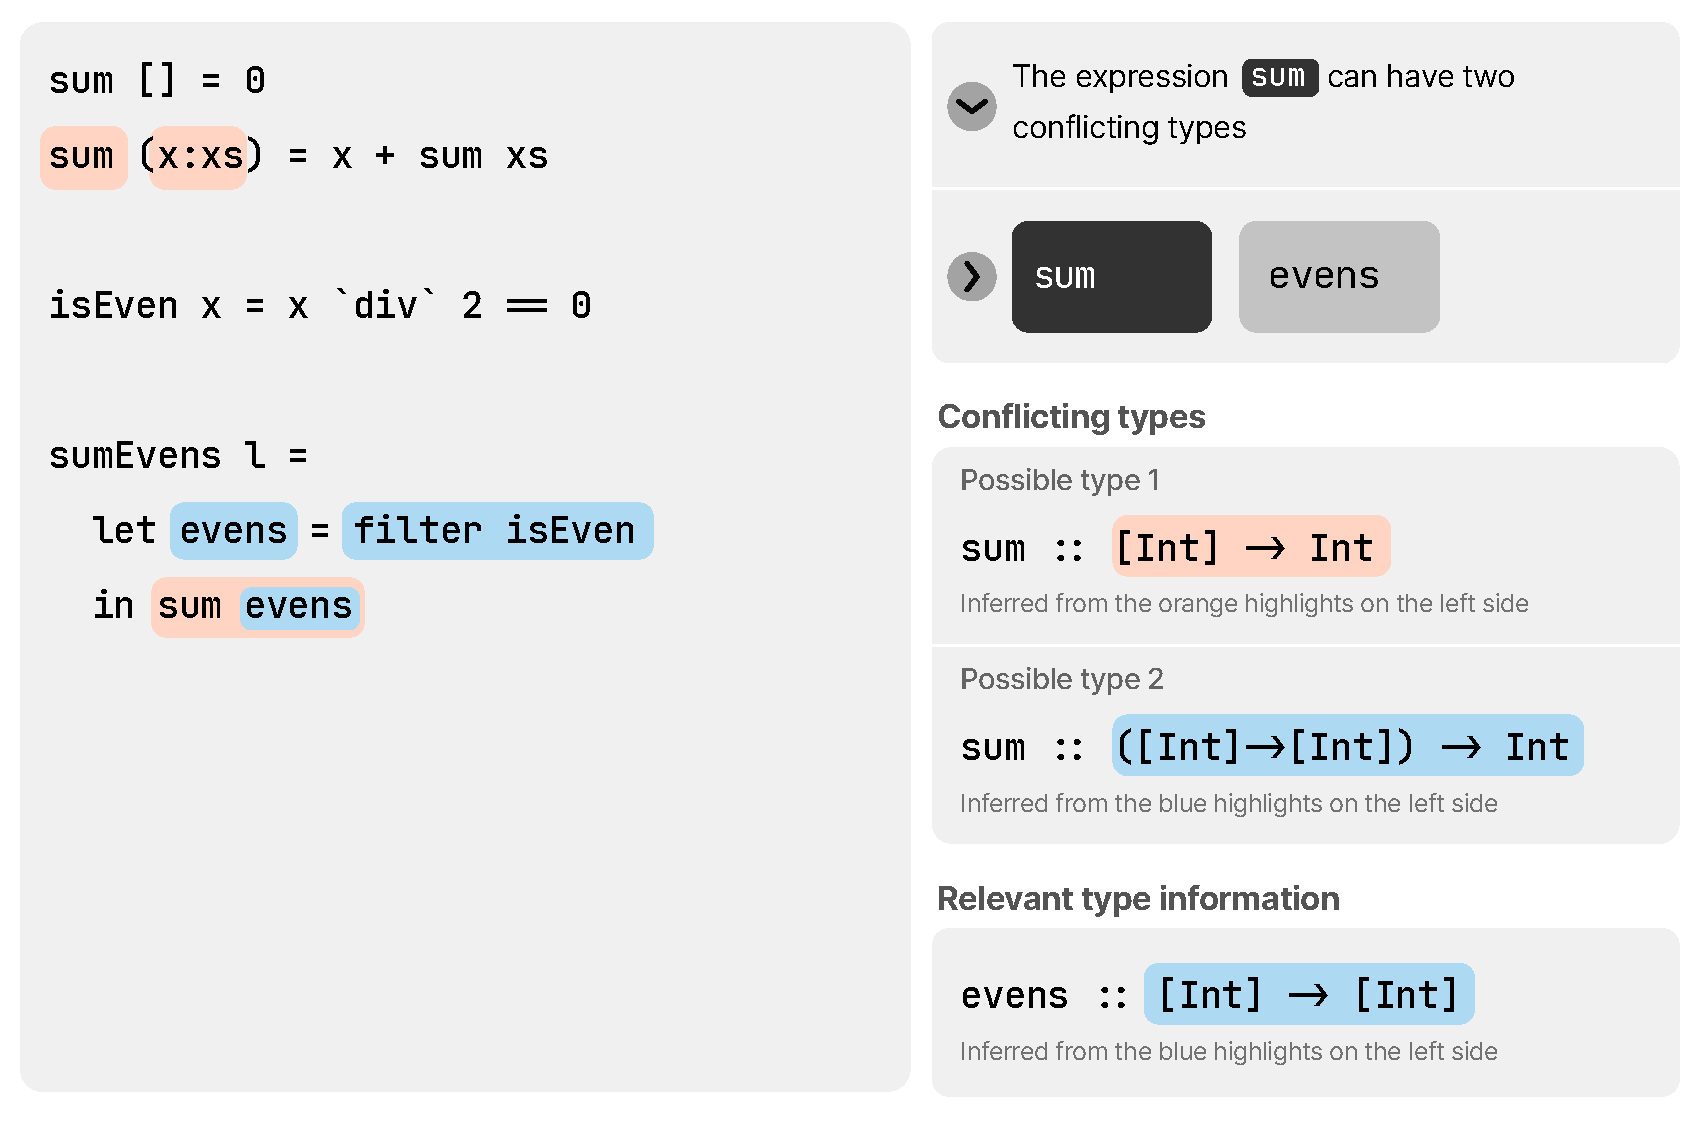
\includegraphics[width=\linewidth]{images/balanced-mode-1.pdf}
        \caption{
            Maxine's code to calculate only the sum 
            of even numbers. \chameleon{} reports 
            an error with two candidate expressions.
        }
        \label{fig:balance-mode-1}
\end{figure}


\begin{figure}
   \centering
        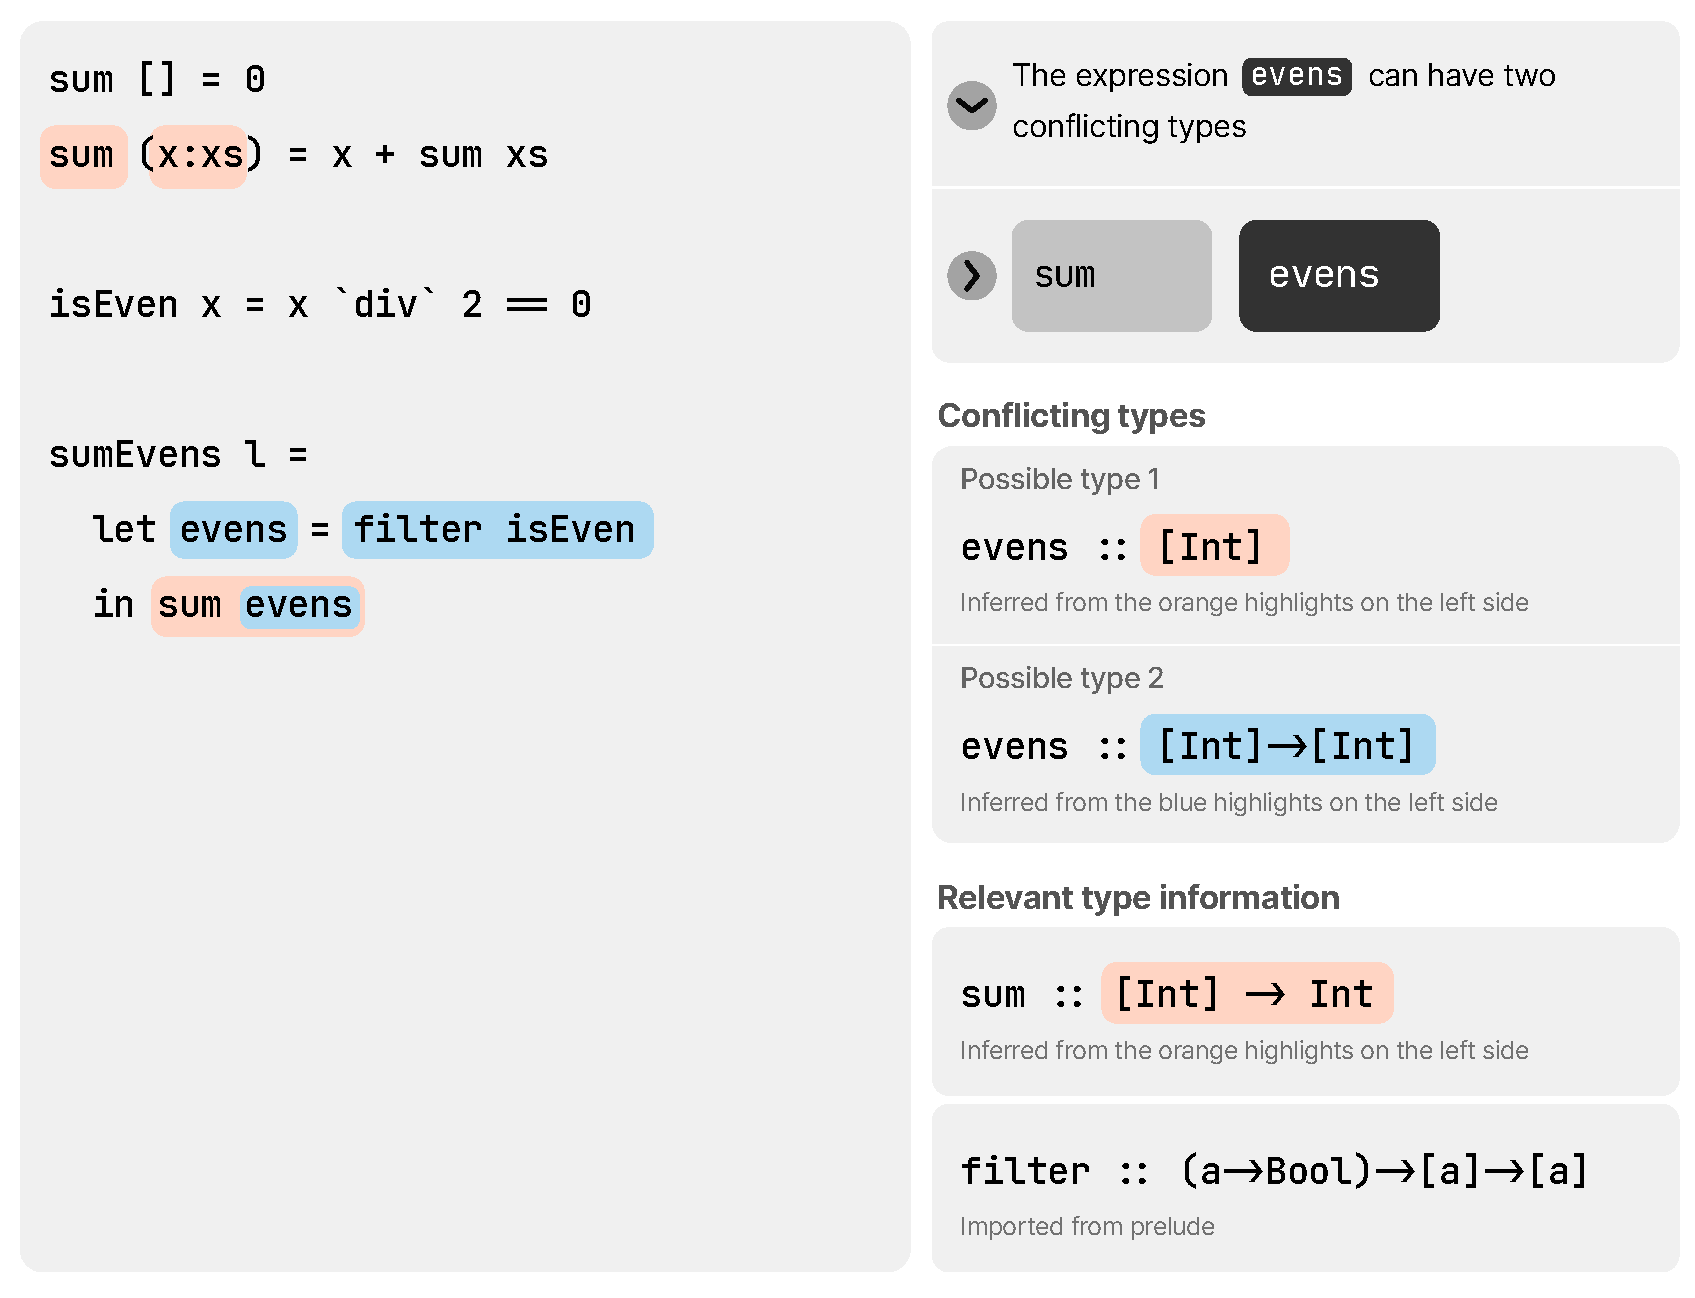
\includegraphics[width=\linewidth]{images/balanced-mode-2.pdf}
        \caption{
            Clicking on the \texttt{evens} card (5) results in the changes in the
            conflicting types panel to show the possible types for \texttt{evens},
            and the changes highlights color to reflect the assumption that the
            definition of \texttt{evens} is the cause of the error.  
        }
        \label{fig:balance-mode-2}
\end{figure}



Maxine therefore clicks on the \texttt{evens} card and \chameleon{} shows two
possible types for the expression \texttt{[Int]} and \texttt{[Int] -> [Int]}
(Fig. \ref{fig:balance-mode-2}). Knowing the expression \texttt{evens} holds
a temporary list of even integers (hence it is of \texttt{[Int]} types), Maxine
knows the Possible type 2 is unintended, and blue in-text highlights must
contain the cause. It does not take long until Maxine realizes that the list 
\texttt{l} is not supplied to the \texttt{filter} function.


\subsection{Advanced mode}  \label{sub:advanced}


For the task shown in section \ref{sub:balanced}, if Maxine is not satisfied by
the options provided by \chameleon{}, by switching to advanced
mode, Maxine has access to the debugging steps and the explanation layer. 

\begin{figure}
        \centering
        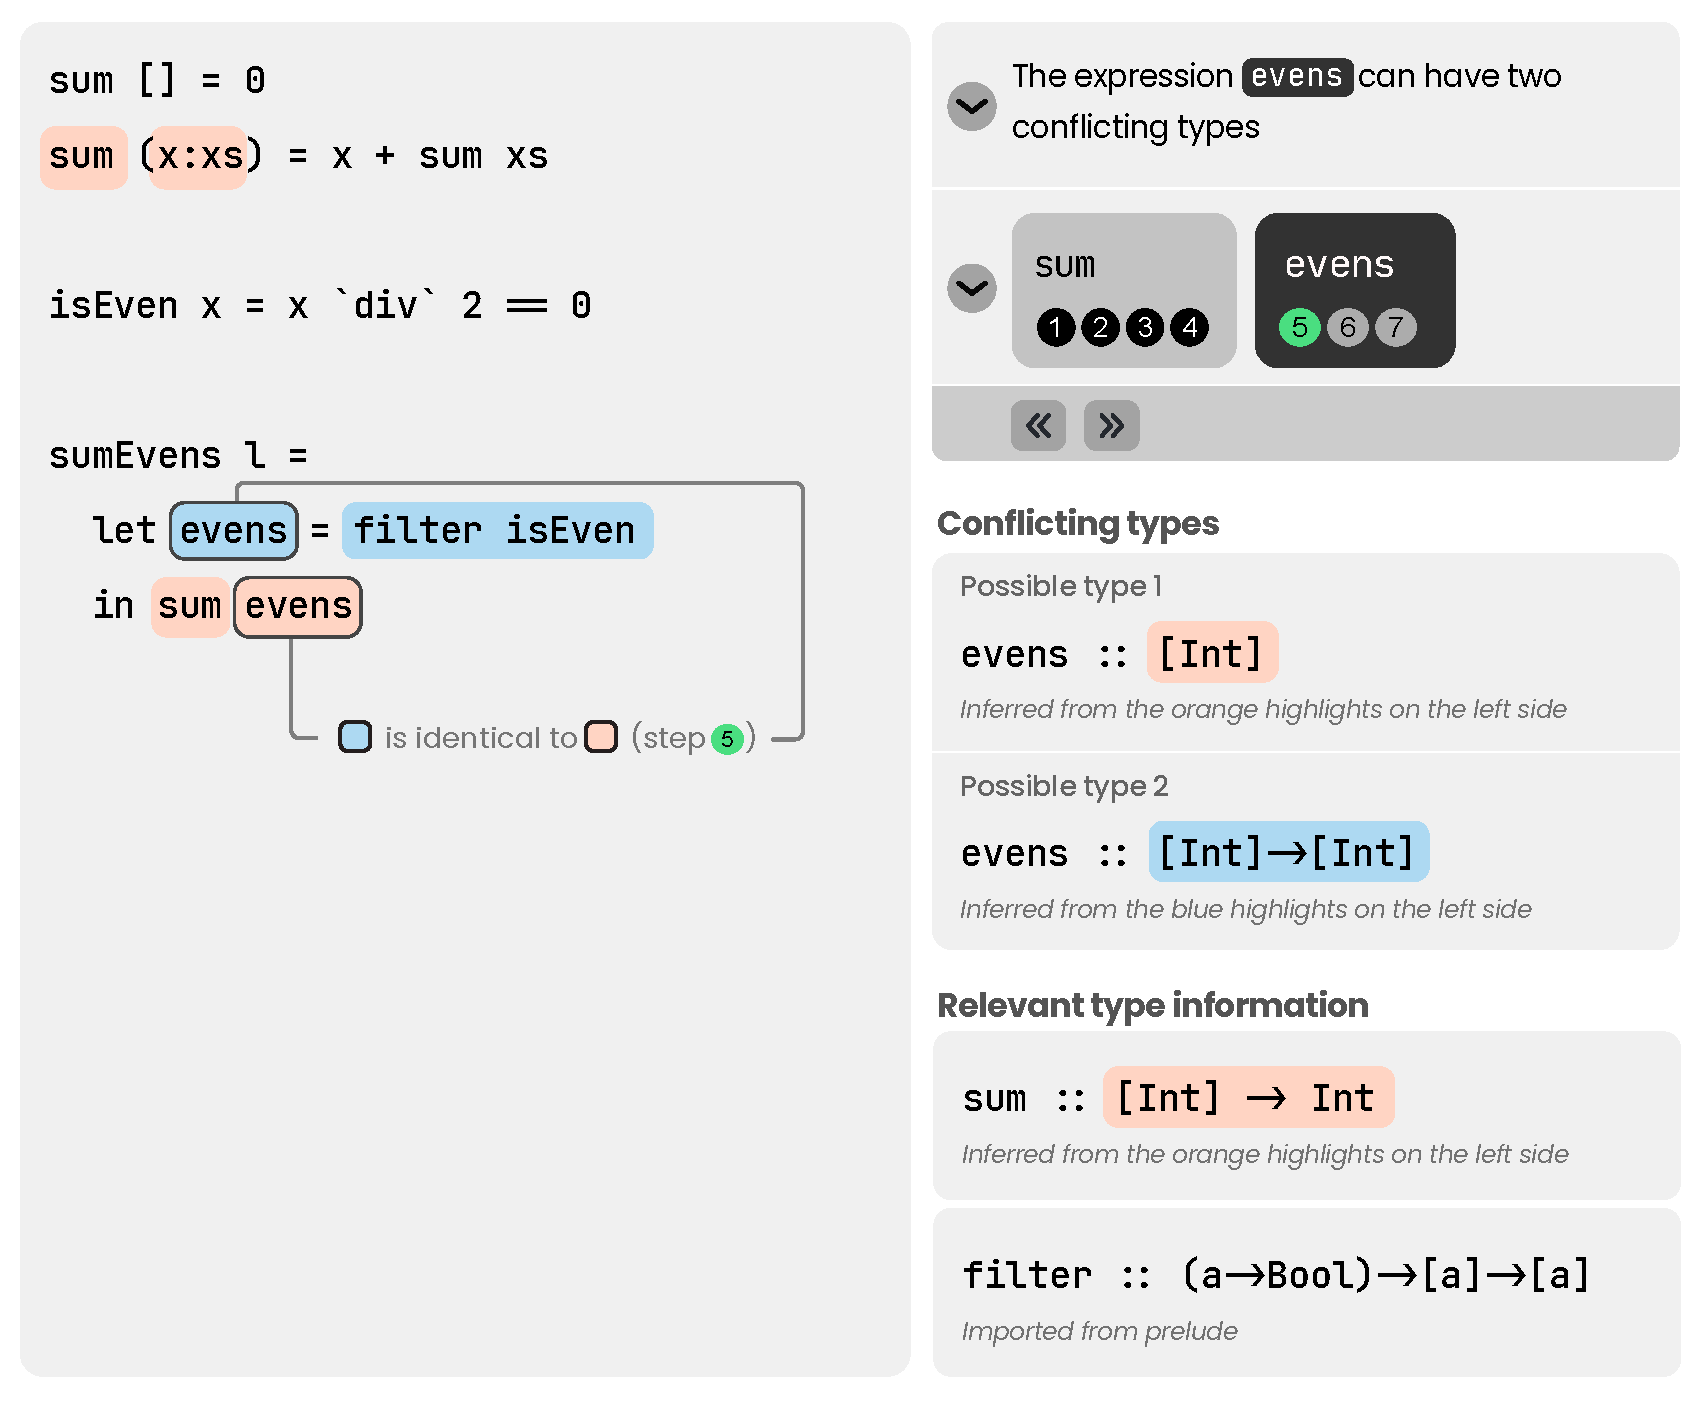
\includegraphics[width=\linewidth]{images/advanced-mode-1.pdf}
        \caption{
            Maxine's code to calculate only the sum 
            of even numbers in advanced mode. 
            The current step is step 5, \chameleon{} 
            explains that the two appearances of expression 
            \texttt{evens} should have the same type.
        }
        \label{fig:advanced-mode-step5}
\end{figure}

\begin{figure}
        \centering
        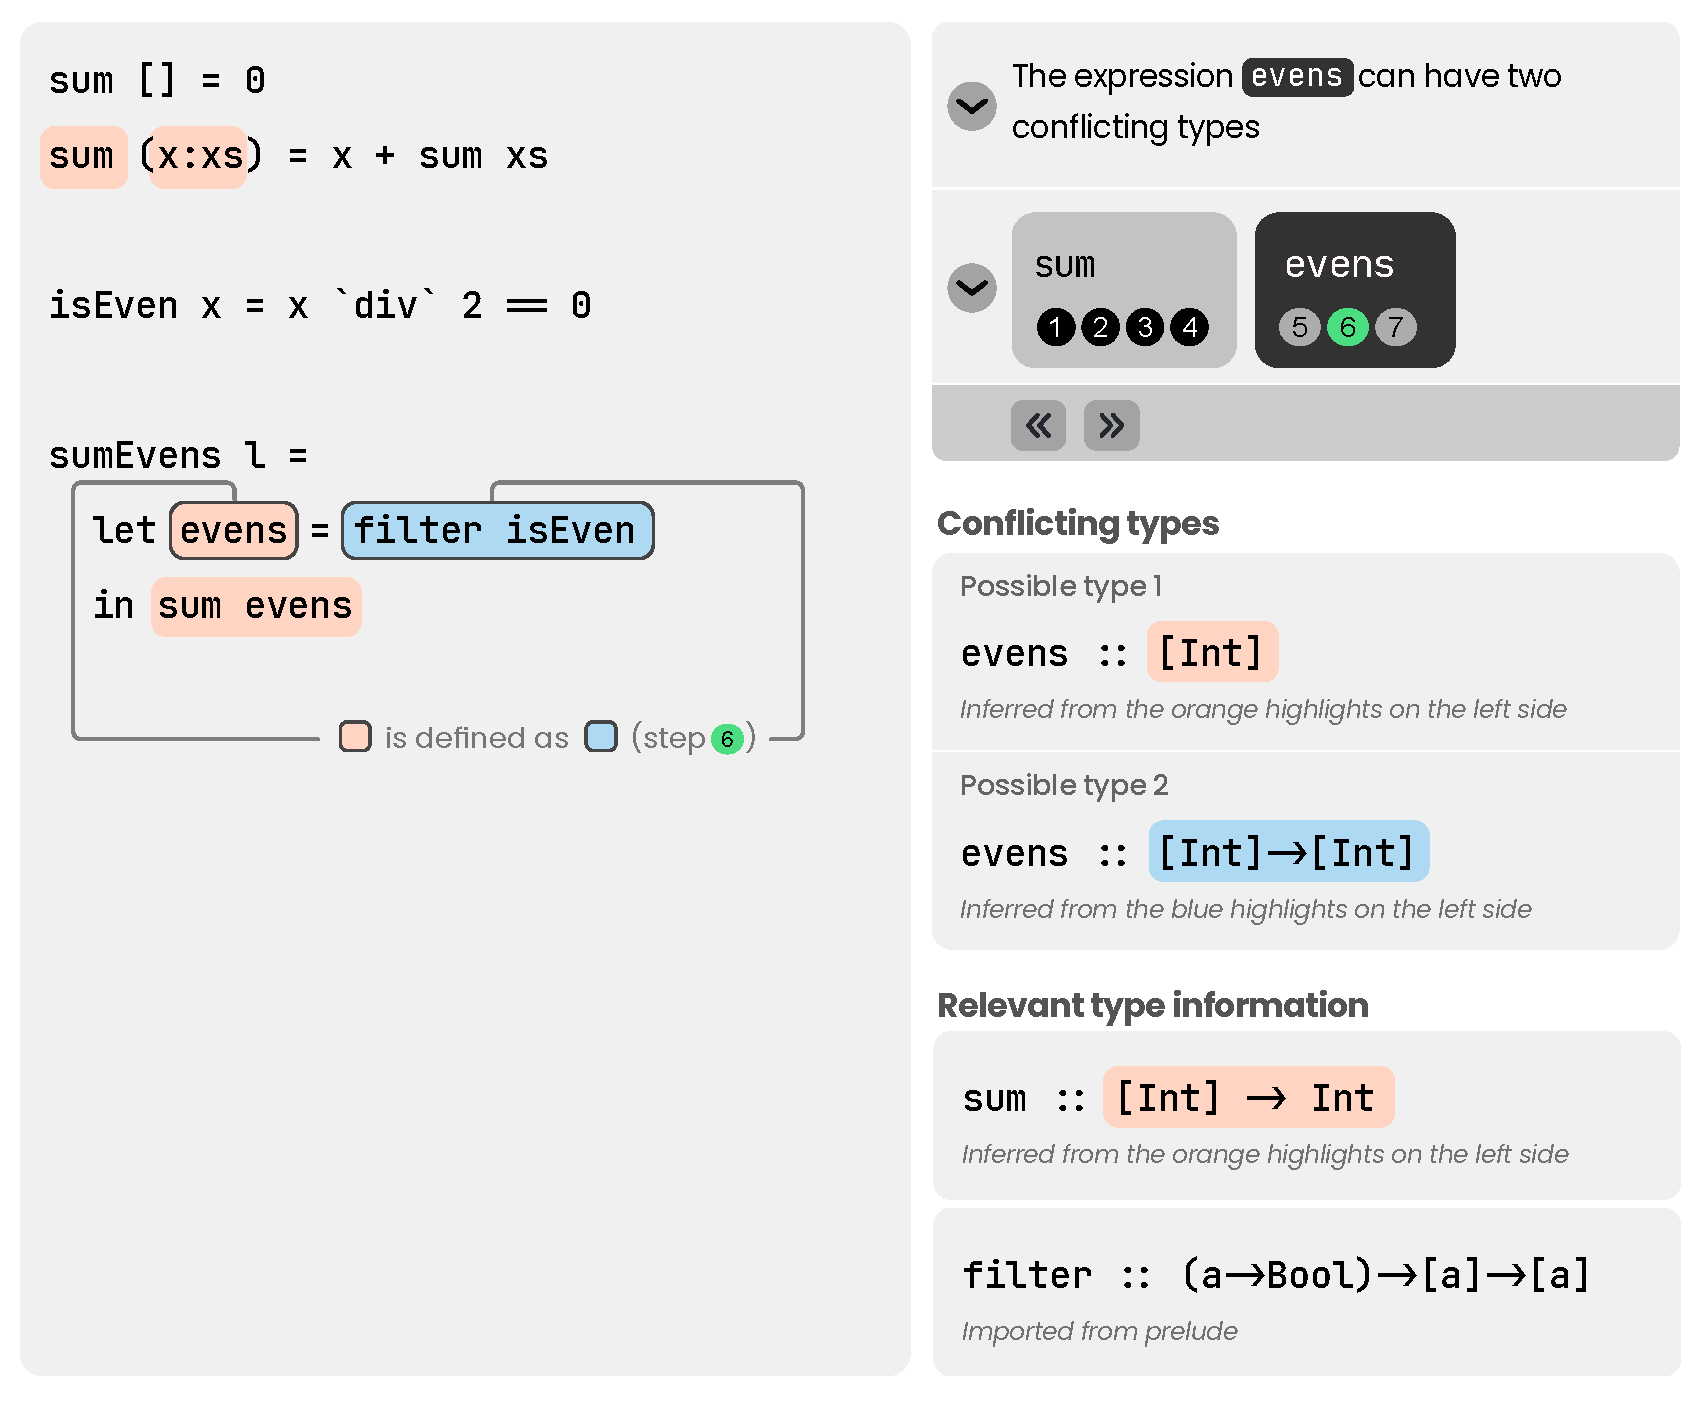
\includegraphics[width=\linewidth]{images/advanced-mode-2.pdf}
        \caption{
            In step 6, \chameleon{} 
            explains that \texttt{evens} is defined as
            the expression \texttt{filter isEven}. The left-hand side
            and right-hand side should have the same type.
        }
        \label{fig:advanced-mode-step6}
\end{figure}

\begin{figure}
        \centering
        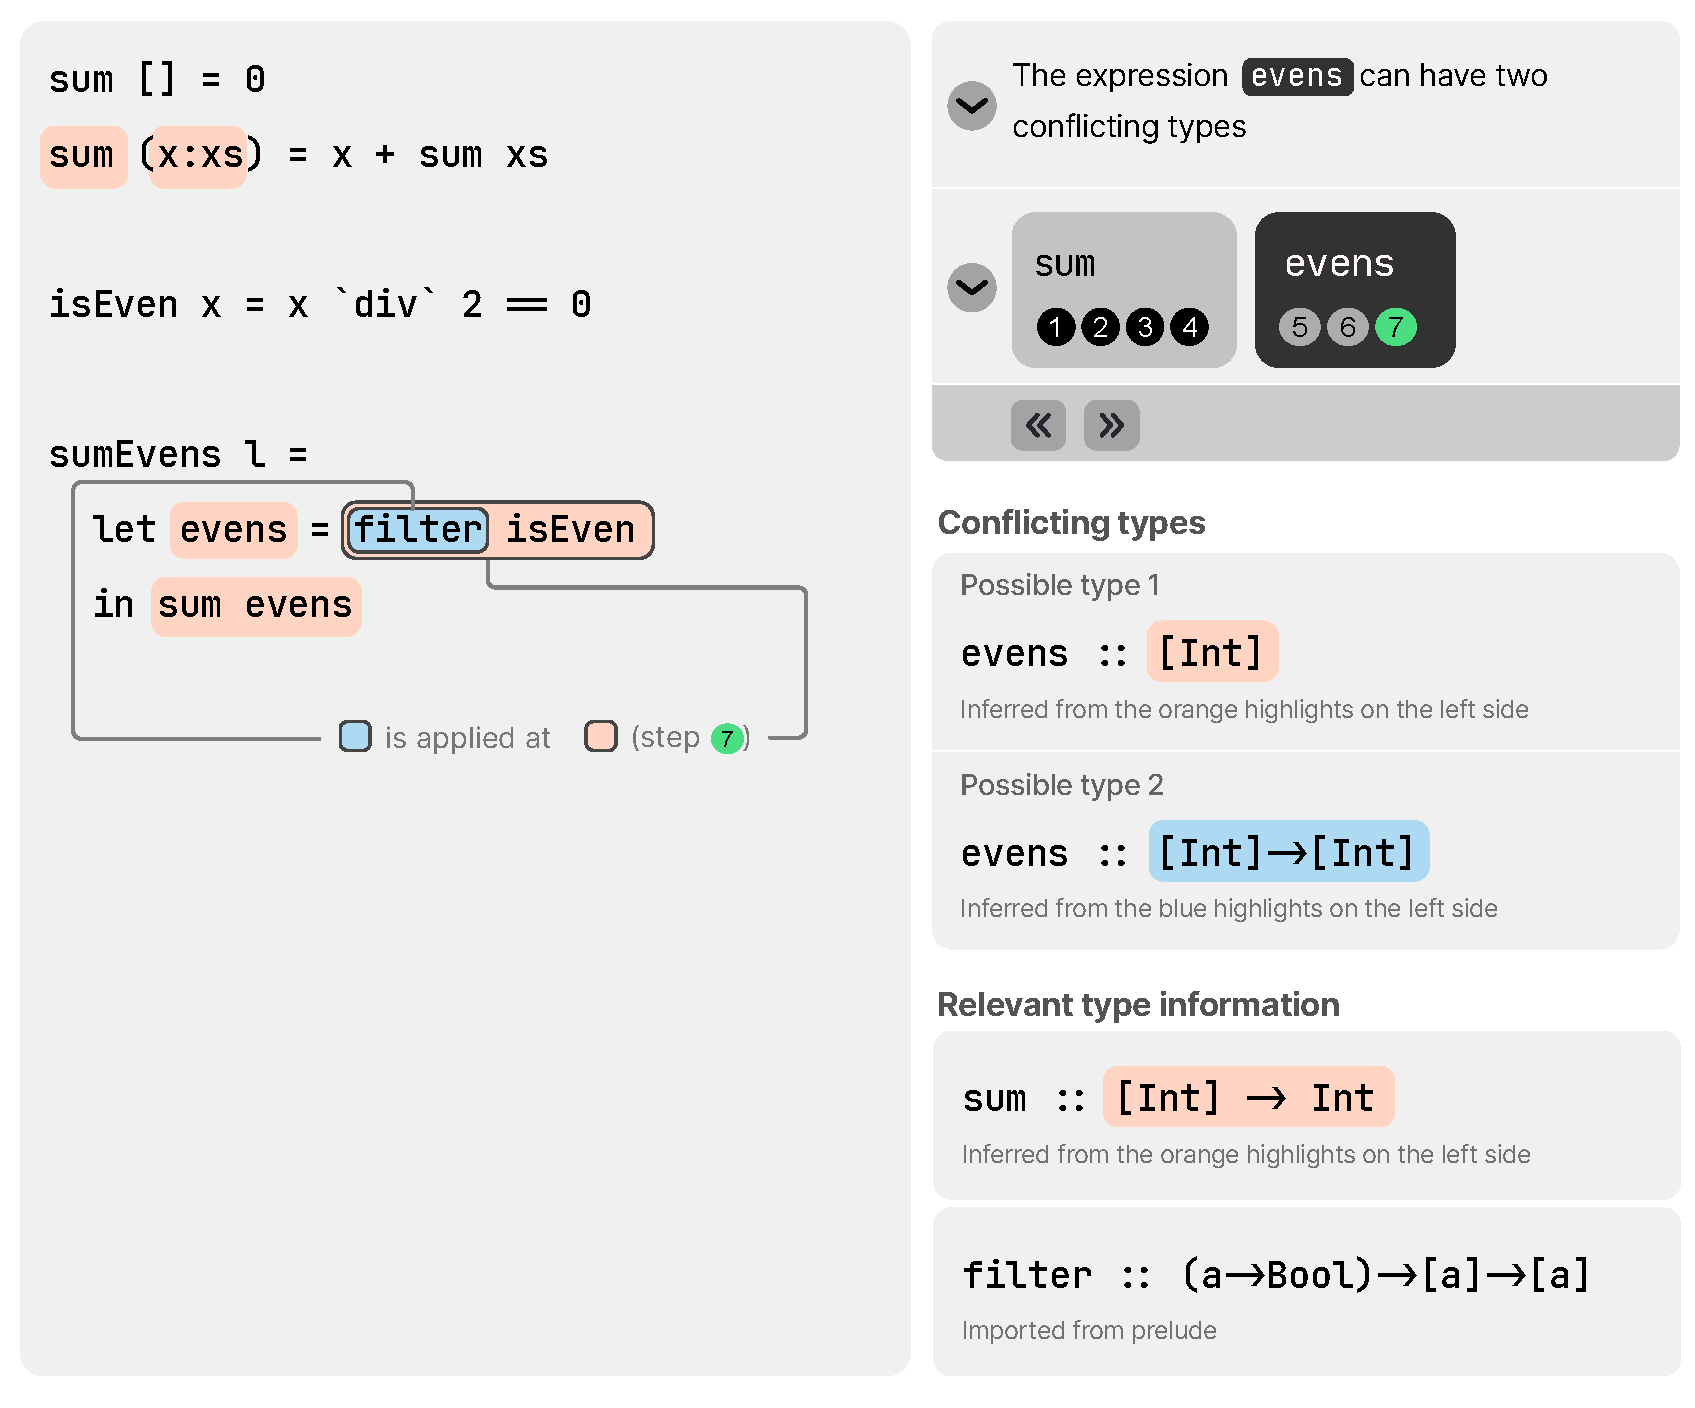
\includegraphics[width=\linewidth]{images/advanced-mode-3.pdf}
        \caption{
            In step 7, \chameleon{} 
            explains that \texttt{filter} is applied to 
            the function \texttt{isEven}. Assisting by 
            the type of \texttt{filter} in the 
            Relevant Type Information panel on the bottom
            right, Maxine can find the type error that 
            \texttt{filter} expects two arguments but receives one.
        }
        \label{fig:advanced-mode-step7}
\end{figure}



First, Maxine clicks on step 5 (Fig. \ref{fig:advanced-mode-step5}) and verifies
that the two occurrences of \texttt{evens} are supposed to be identical, and the
second usage dictates that \texttt{evens} is a list of integers. Second, she
clicks on step 6 (Fig. \ref{fig:advanced-mode-step6}) and verifies that
\texttt{evens} should be the same type as the declaration on the right-hand
side. 


Lastly, Maxine clicks on step 7 (Fig. \ref{fig:advanced-mode-step7}), and
it shows that the \texttt{filter} function is applied to one argument
\texttt{isEven}. By consulting the relevant type information, Maxine identifies
that \texttt{filter} is expecting two arguments while only one is provided. 


\section{Evaluation}

Over 12 months, several studies were conducted to answer new research questions or rephrase existing ones. These studies are grouped in 3 phases, each tested a different version of \chameleon{} with human participants. The number of participants and their haskell experience is shown in the table below. 

\begin{figure}[h]
    \centering
    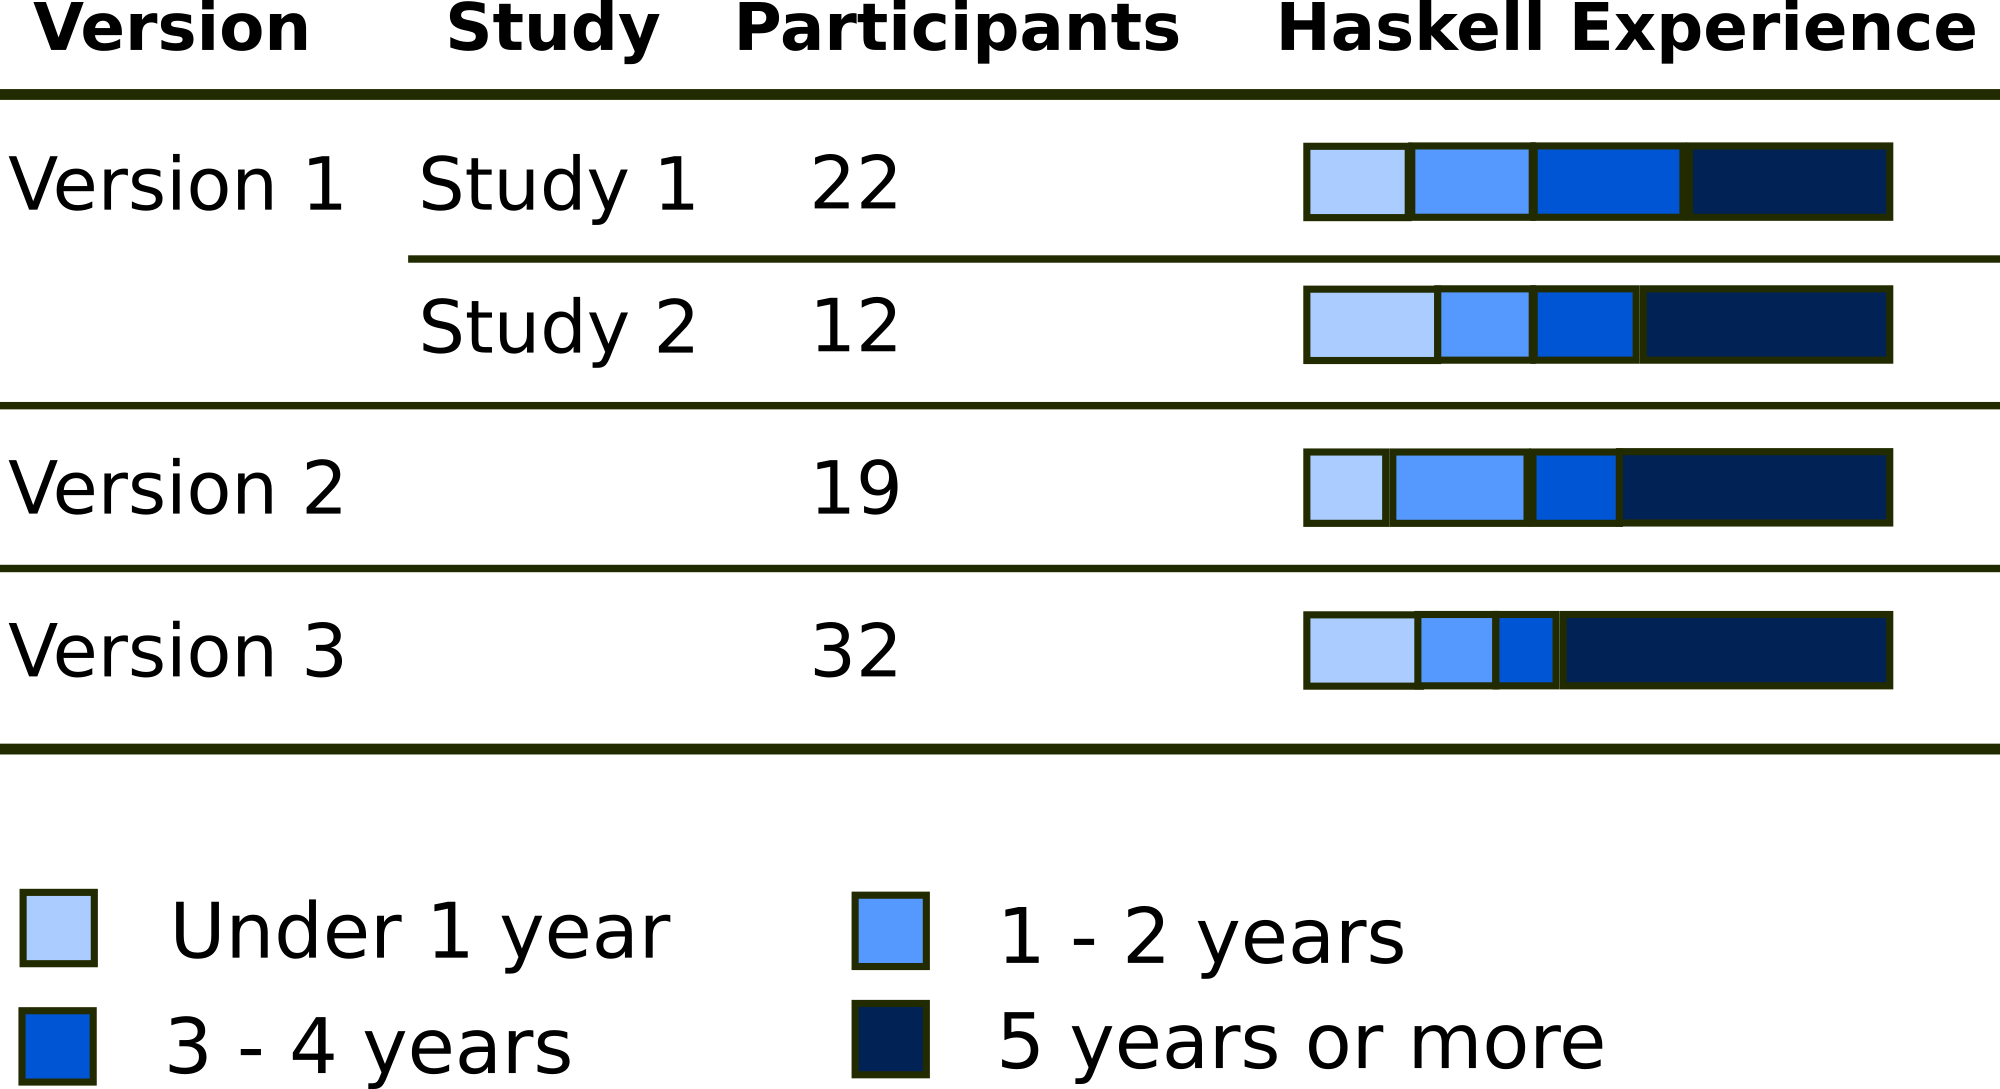
\includegraphics[width=\linewidth]{images/participants-experience.png}
    \caption{}
    \label{fig:participant-experience}
\end{figure}

A summary of the timeline of the user studies, their major questions and conclusions is given in Figure~\ref{fig:timeline}.

\begin{figure}[h]
    \centering
    \Description{A timeline of \chameleon{} evaluations}
    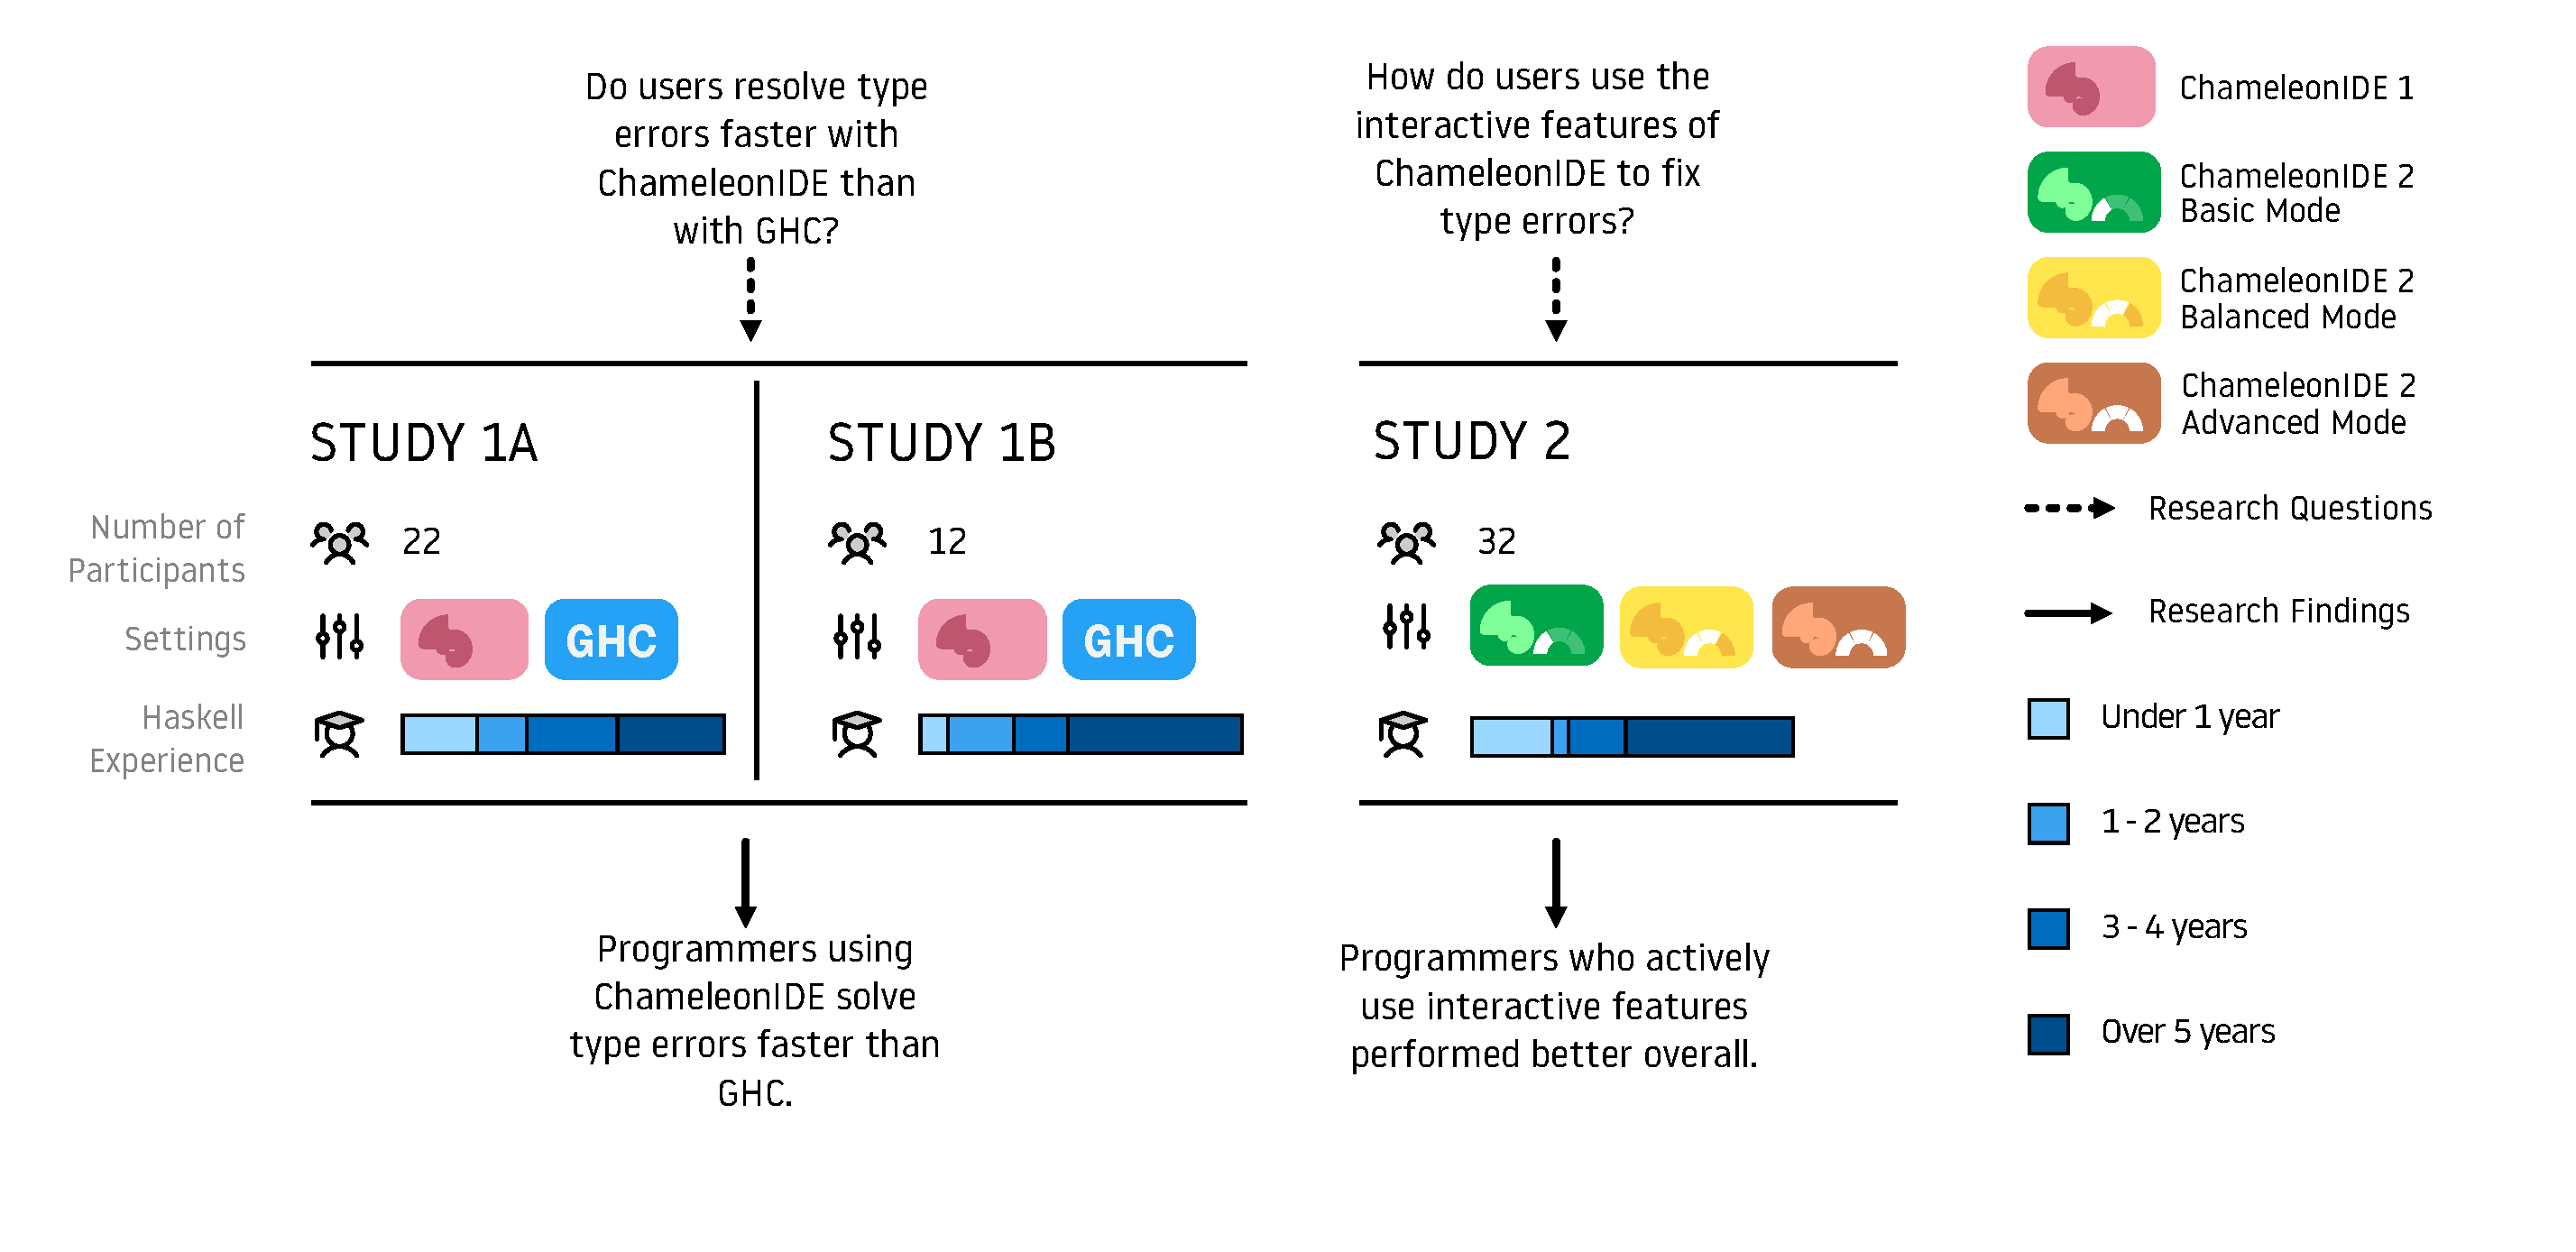
\includegraphics[width=\linewidth]{images/timeline.pdf}
    \caption{The timeline of \chameleon{}  development and 
    evaluation.}
    \label{fig:timeline}
\end{figure}

\subsection{Experiment Design}
\subsubsection*{\textbf{Recruitment}}

Participant recruiting channel was the social news aggregation website Reddit. Specifically, our user study advertisements were posted in the Haskell programming language community "r/haskell" and a general programming language-focused community "r/programminglanguages". Recruiting from social media allowed us to access a more diverse demographic that better represent the true population of Haskell programmers. The participation is fully anonymized. The detailed ethical implications of these experiments are reviewed and approved by the IRB of the institution of the authors.

One consequence of our recruiting approach is it is harder for previous participants to enter an later study. To minimise the lurking variable of previous experience, we use new code challenge every study and conduct trial runs in every study to bring new participants up to speed.

\subsubsection*{\textbf{Experiment setting}}
The experiment took place remotely and unsupervised. Participants took the study online via web browser and at the physical venue of their choosing. All user studies use a web-based debugging environment developed by the authors. Conducting the studies online helped us avoid variation when performing tasks in unfamiliar places and using different setups. The downside is that to intervene when a user encounters bugs or usability issues mid-study is impossible. To ensure there is no major usability issue that could lower the quality of data collection, we conducted cognitive walkthroughs and sandbox pilots before running each study.

\begin{figure}[h]
    \centering
    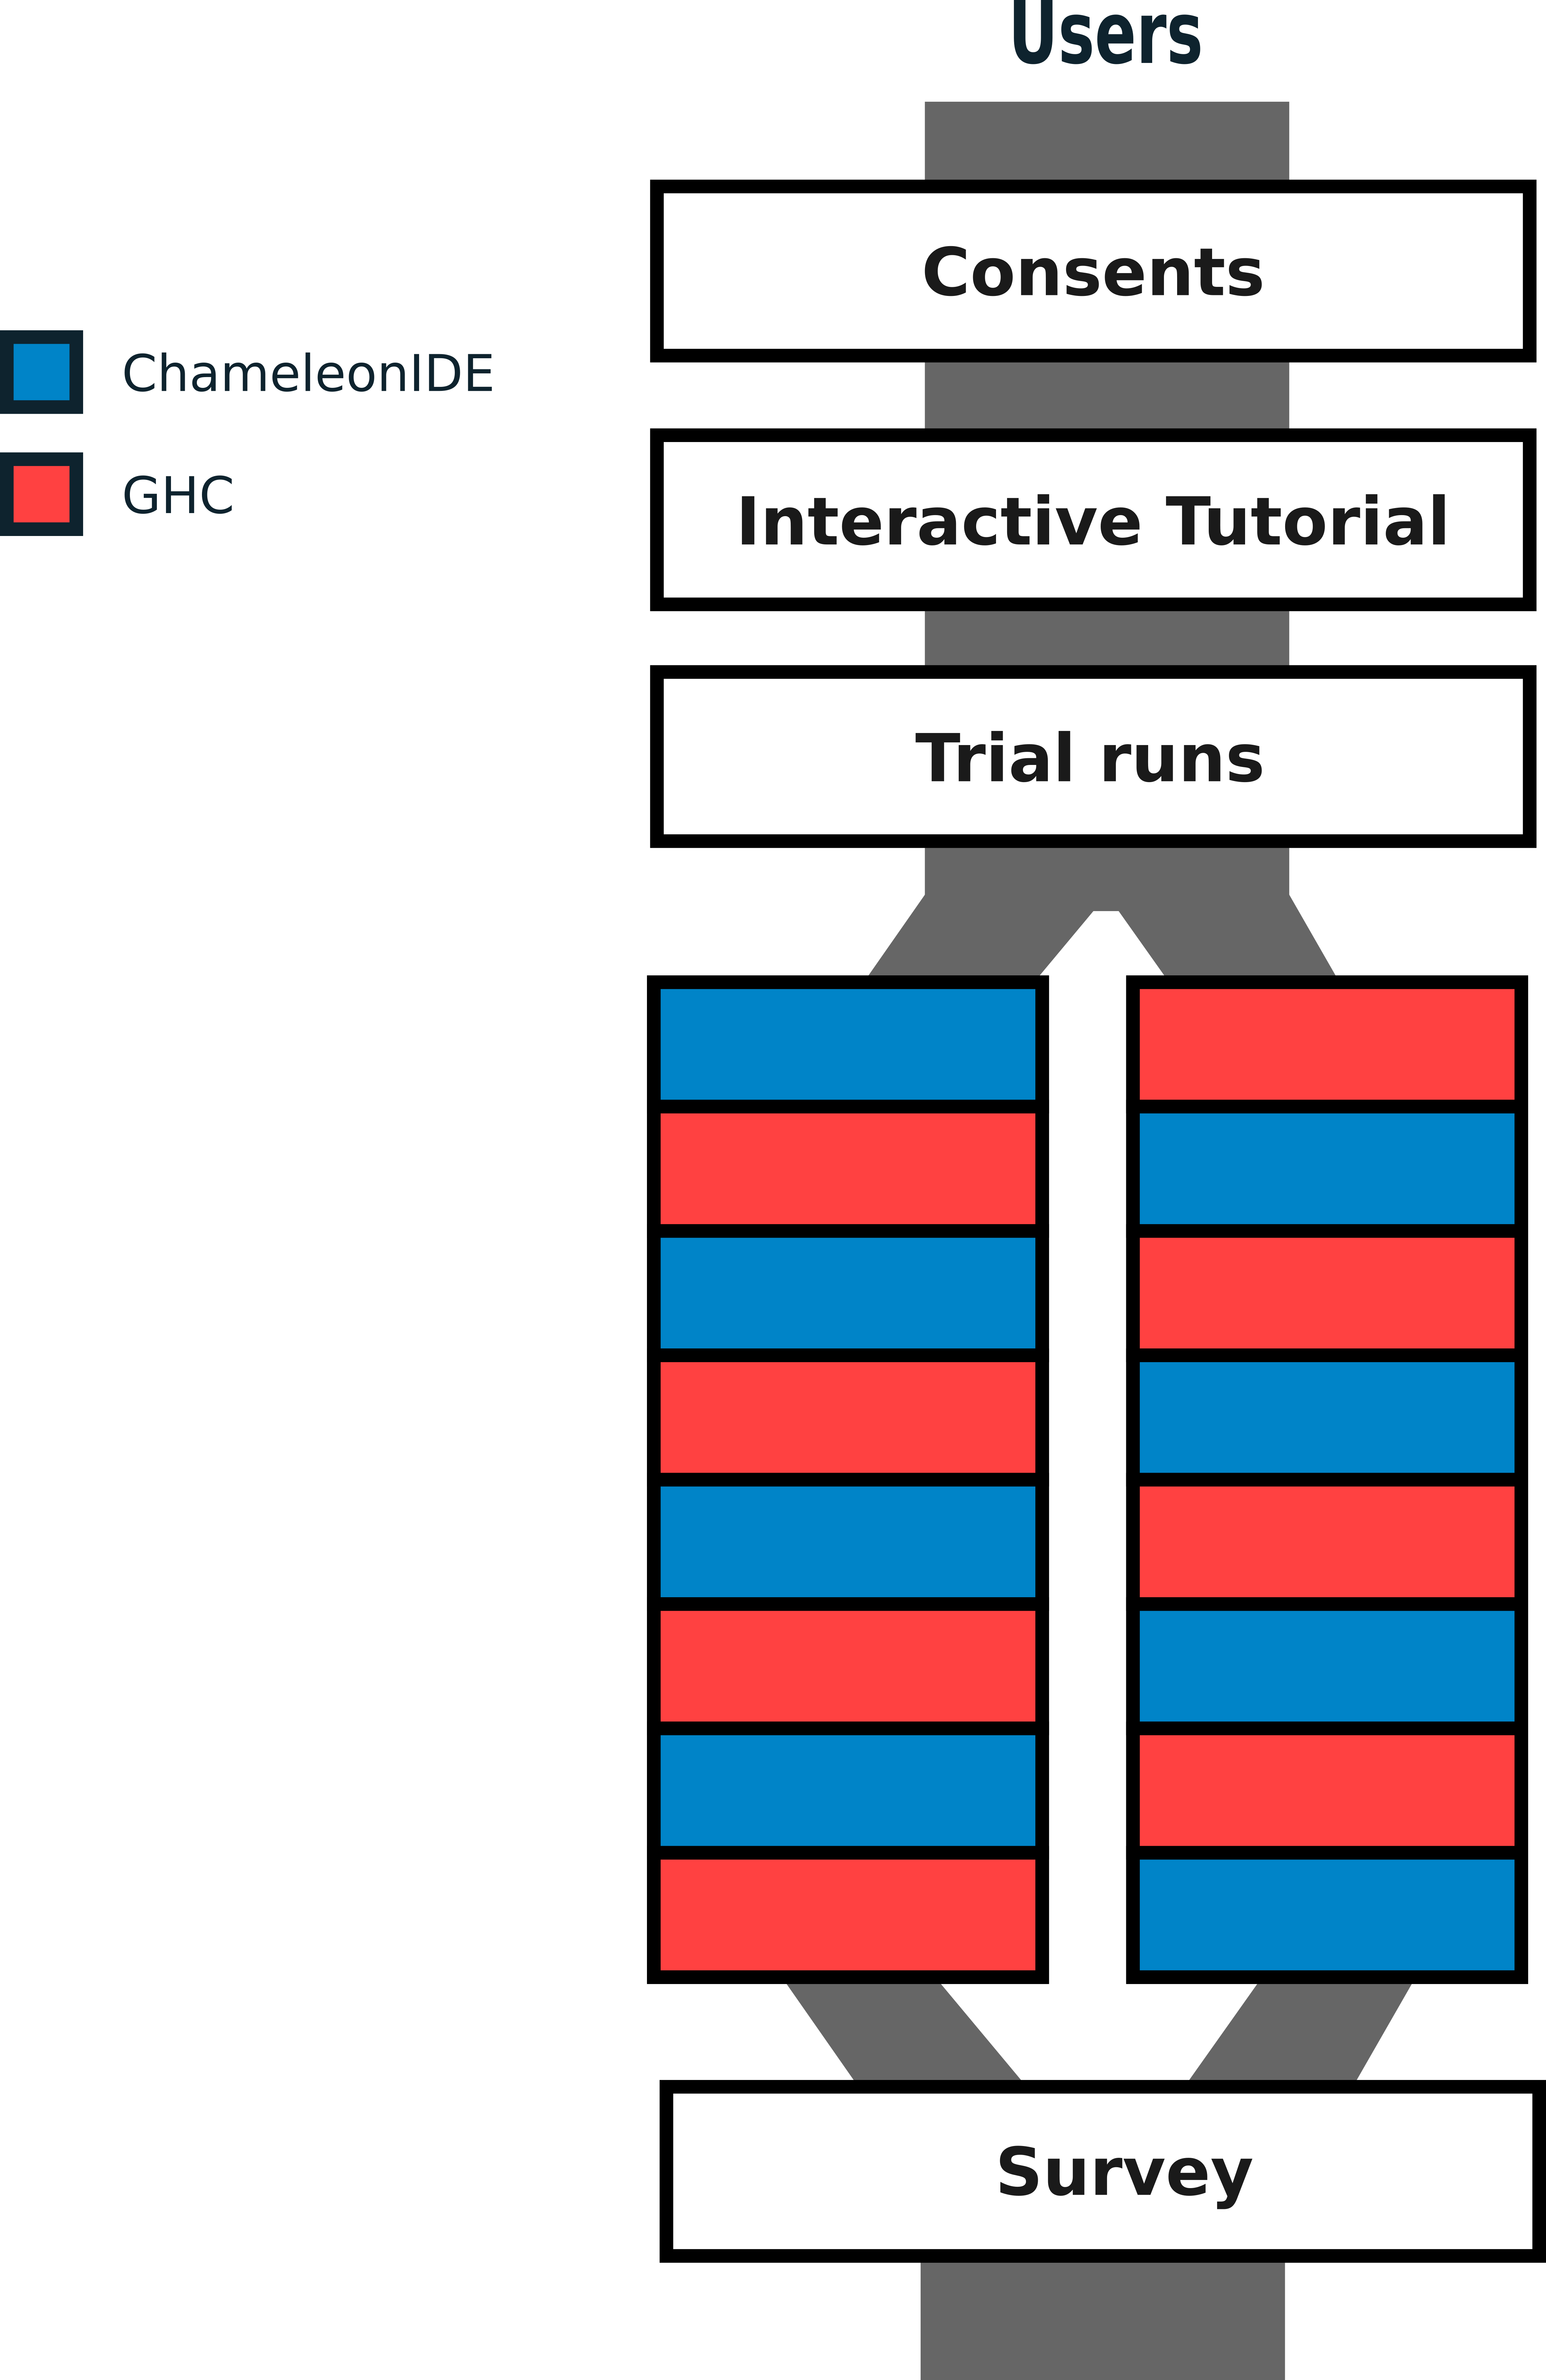
\includegraphics[width=\linewidth]{images/study-process.png}
    \caption{}
    \label{fig:study-process}
\end{figure}

\subsubsection*{\textbf{Training and group assignment}}
After consent, participants received interactive training on every function of the tool interface and interactive features. Participants were also shown the important functionalities of the tool interface in a summarized cheat sheet. Participants had access to the cheat sheet at all times during the study. Participants were given 4 trial runs (2 for each setting) before the data collection starts. 

All the user studies used a within-subject design to evaluate the effectiveness of different tools or feature sets while counterbalancing the difference in programming proficiency between participants. In each user study, participants were required to complete a series of programming tasks (8 for user studies 1 - 3, 9 for user study 4). At each task, a participant receives a single Haskell file that contains one or more type errors. The participant was asked to make the code type check with the help of the tool given for this task.


% During each study, a participant received two (user studies 1 - 3) or three (user study 4) different debugging tools. The debugging tools were different systems (user studies 1 - 3) or different feature sets of the same system (user study 4). For each participant, the debugging tools alternative through consecutive tasks to ensure the fatigue level does not impair the rigorousness of data collection.

\subsubsection*{\textbf{Measurement}}
Time is measured from the start of each task to the first time the program is successfully type-checked and also passes all the functional tests. The data is automatically recorded by the online debugging environment. To not introduce a barrier to completing the study, every task can be skipped if the participant made three attempts or spent over 1 minute on the task.


After completing all the tasks (8 in user studies 1-3, 9 in user study 4), users are prompted to fill in a debriefing survey. The survey questions include their Haskell programming experience and feedback on the tools and feature sets participants used during the study.


We used an browser session recording tool~\cite{openreplay} to record the user study sessions. These recordings are used to find usability issues in the study and recognize general patterns. However, the recording technology does not provide high enough sampling rate for us to be confidently used for rigorous analysis.

\subsection{\chameleon{} User Studies}


\subsubsection{\textbf{Version 1}}  
\chameleon{} version 1 provides the rewrite of the Chameleon type inference engine and the type compare tool to show the alternative types and possible error locations in matching colors.

\begin{figure}[h]
    \centering
    \Description{Chameleon v1}
    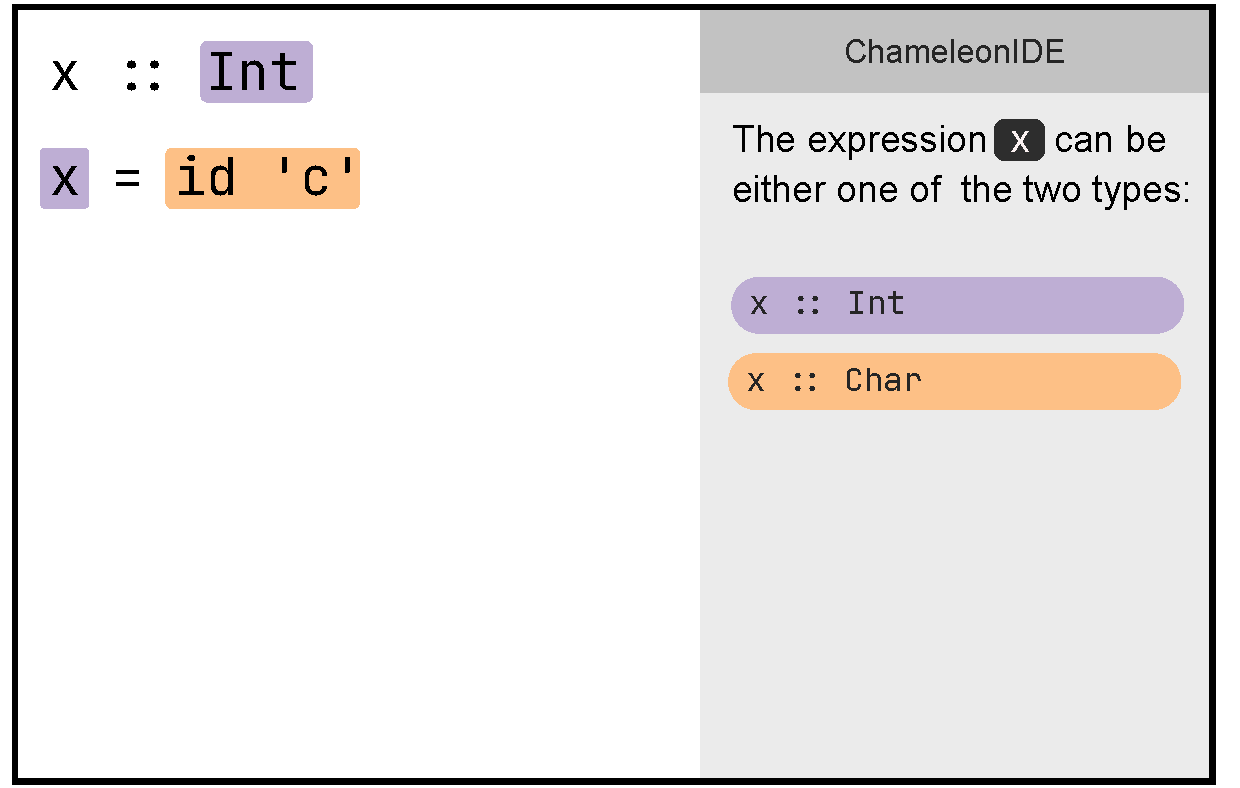
\includegraphics[width=\linewidth]{images/chameleon-v1.pdf}
    \caption{
        \chameleon{} Version 1
        }
    \label{fig:chameleon-v1}
\end{figure}

Two user studies were conducted to test \chameleon{} version 1, to compare the effectiveness of solving type errors using \chameleon{} and GHC compiler error messages. We choose GHC compiler error messages as the baseline because it is the canonical tool for working with type error in Haskell. Although high-level tools like Haskell Language Server exist, they generally relay the GHC error messages verbatim. 


Eight tasks were given in both studies. In the first study, the tasks were taken from a exercises from the exercises of the Haskell programming units. These tasks cover a variety of type errors. \tf{break down the type error classes.} However these tasks, as shown from the result and feedback of user study 1, were too simple to fully evaluate the two options. In the second study, the tasks are sourced from the top 20 Haskell topics on GitHub~\cite{githubHaskell}. The authors manually added type errors. 


% The study investigates the effectiveness of \chameleon{} compared to the GHC compiler error messages. We chose GHC compiler error messages as it is the canonical tool for debugging type errors in Haskell. Although high-level tools like Haskell Language Server exist, they relay the GHC error message verbatim for type errors. Participants are asked to complete 8 tasks. The tool participants used during each task alternated between \chameleon{} and GHC. Task programs were sourced from HaskellWiki \cite{haskellwiki}. The author manually added type errors. The errors cover a range of common Haskell type errors, including abstract data types, wrong arity, control expressions (if and case), infinite types, and tuples. The lines of code (LoC) range from 7 to 17 (mean = 11, median=10.5).


% In total 39 participants finished the study. Among them, 12 participants have over five years of Haskell experience, and 5 participants have three or four years of Haskell experience. And 8 participants have one or two years of experience, and 5 participants used Haskell for under a year. The rest left the question unanswered.

\begin{figure}[h]
    \centering
    \Description{Time to complete by task in user study 1 with confidence interval}
    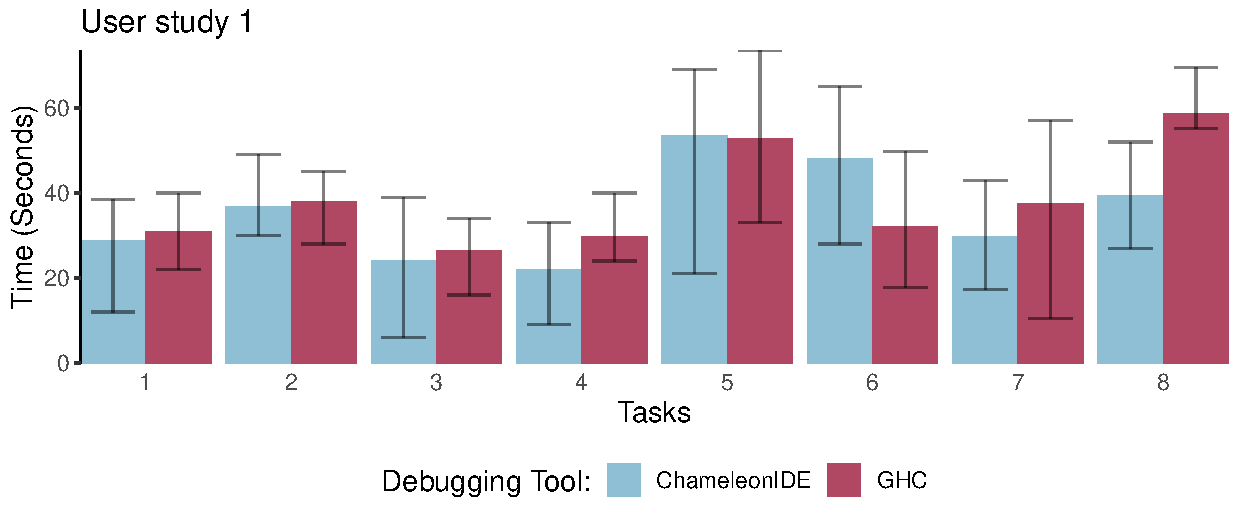
\includegraphics[width=\linewidth]{images/r1-data.pdf}
    \caption{Time to complete by task in user study 1 with confidence interval}
    \label{fig:r1-analysis}
\end{figure}


\begin{figure}[h]
    \centering
    \Description{Time to complete by task in user study 2 confidence interval}
    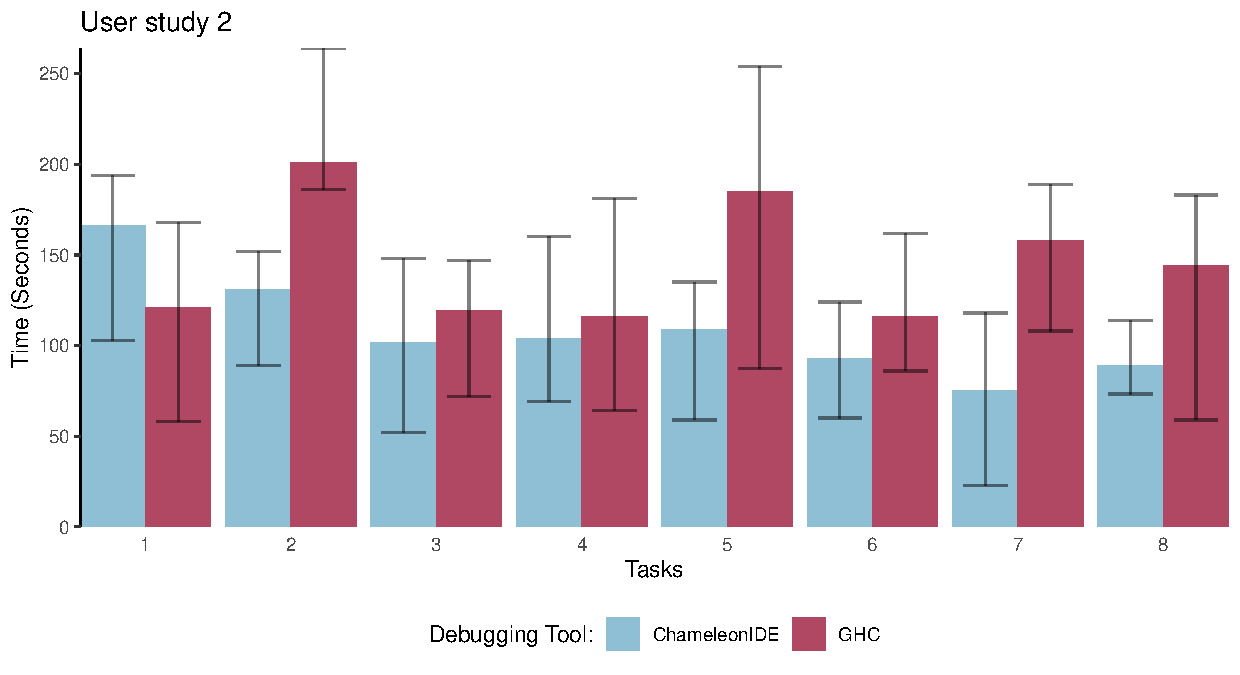
\includegraphics[width=\linewidth]{images/r2-data.pdf}
    \caption{Time to complete by task in user study 2 confidence interval}
    \label{fig:r2-analysis}
\end{figure}

\subsubsection*{\textbf {Results}}

From the data collected during user study 1 (\ref{fig:r1-analysis}), we could not identify which group performed better (p-value =0.2041, Wilcoxin signed test). For the trivial challenges we set for users, the individual differences are generally more significant than differences between treatments. 
The most common feedback (7 out of 35) from the user study 1 was that the tasks were too trivial to invite meaningful evaluation. One participant put it, "Looks nicer than GHC, but without trying it on something more complicated, I cannot conclude whether it would help me in practice".

One interesting exception is task 8, where the \chameleon{} group outperformed the GHC group more consistently and with a larger effect size (p-value = 0.002456, Wilcoxin signed test). The discrepancy is thought to be related to the nature of Task 8:
\begin{itemize}
    \item {It has a longer source file than other tasks (only shorter than task 6, but task
    6 contains two independent type errors while task 8 is one connected task
    error);}
    \item {It is more complex than others (involves abstract data types and function application); and
    }
    \item {
        GHC struggles to produce a relevant error message for this type of error.
    }
  \end{itemize}
It can be further shown by examining the process some participants took to solve the problem.

  

% \begin{figure}[H]
%     \centering
%     \Description{A screenshot from user study 1}
%     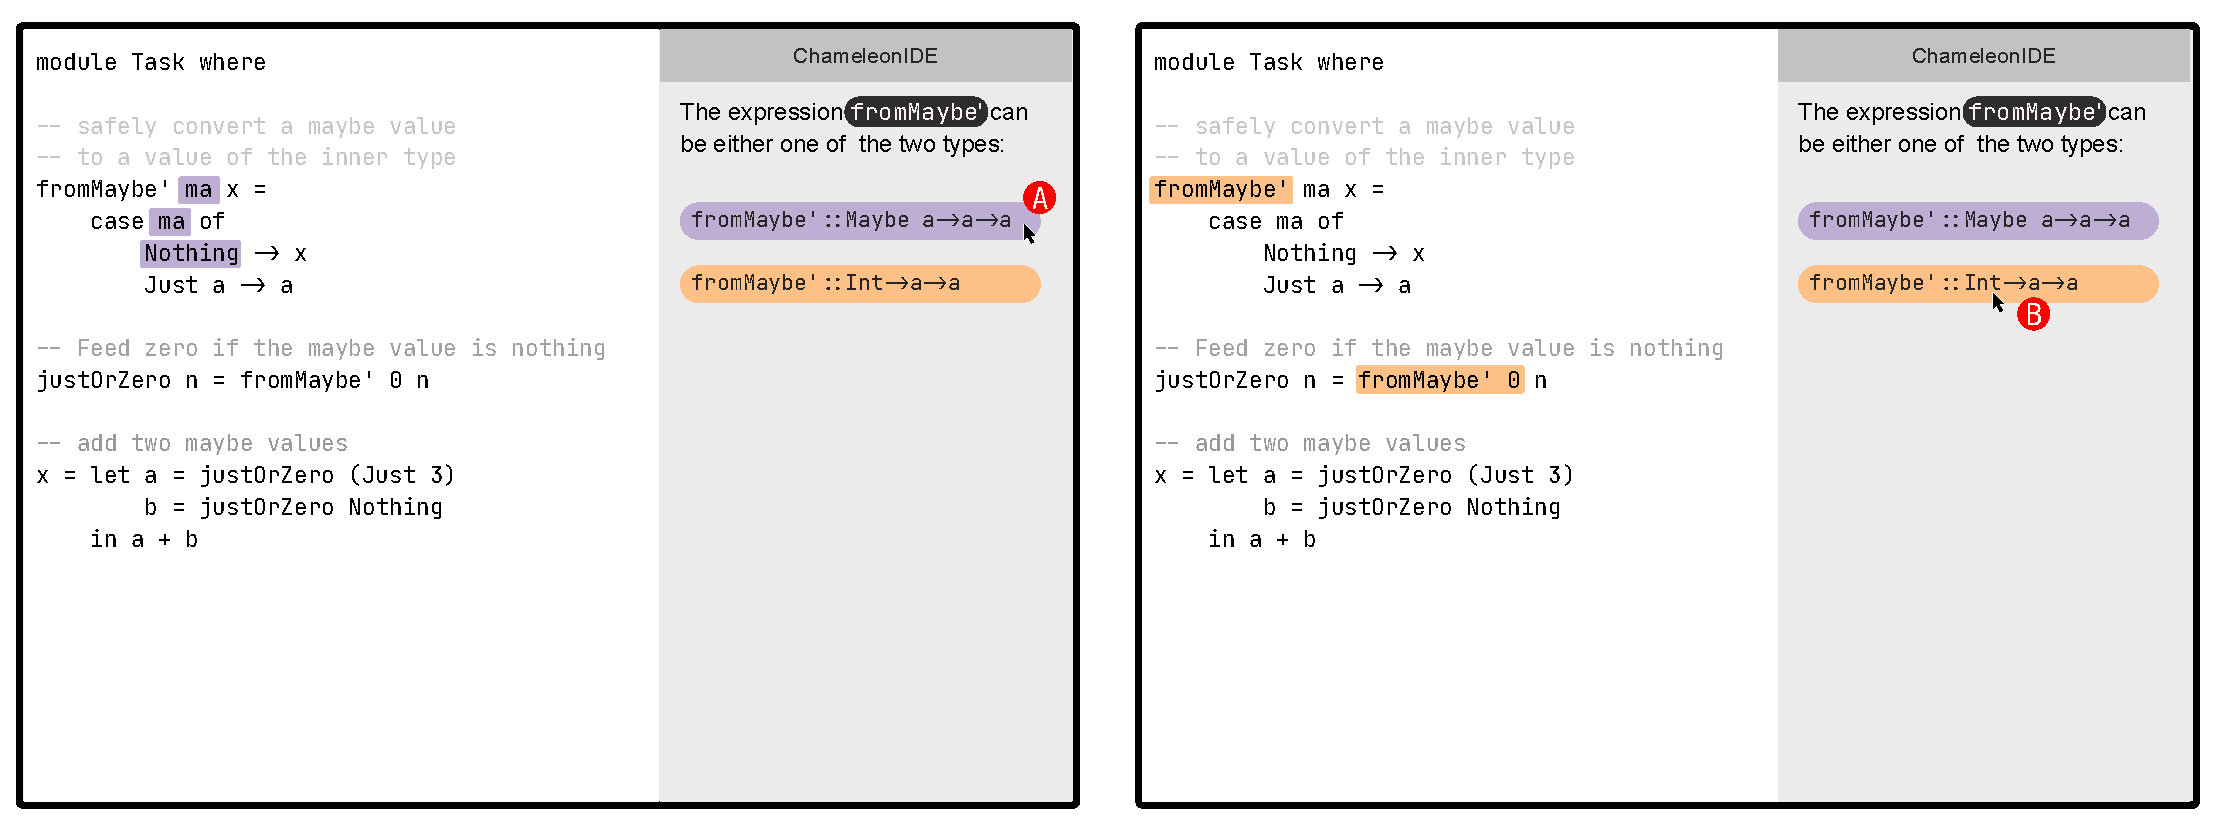
\includegraphics[width=\textwidth]{round1-screenshot.pdf}
%     \caption{
% One participant working with \chameleon{}  managed to identify the most probable location of the error (the application of `fromMaybe'` on line 11) by hovering over the two alternative types. The participant then quickly realized that the first argument `0` (highlighted in orange) is inconsistent with the definition where it is case matched to a `Nothing` value (highlighted in purple). After two retries with short hesitation the participant found the correct fix (by reversing the order of `0` and `n`).
%     }
%     \label{fig:r1-task8}
% \end{figure}


% \begin{figure}[htb]
%     \centering
%     \Description{A screenshot from user study 1}
%     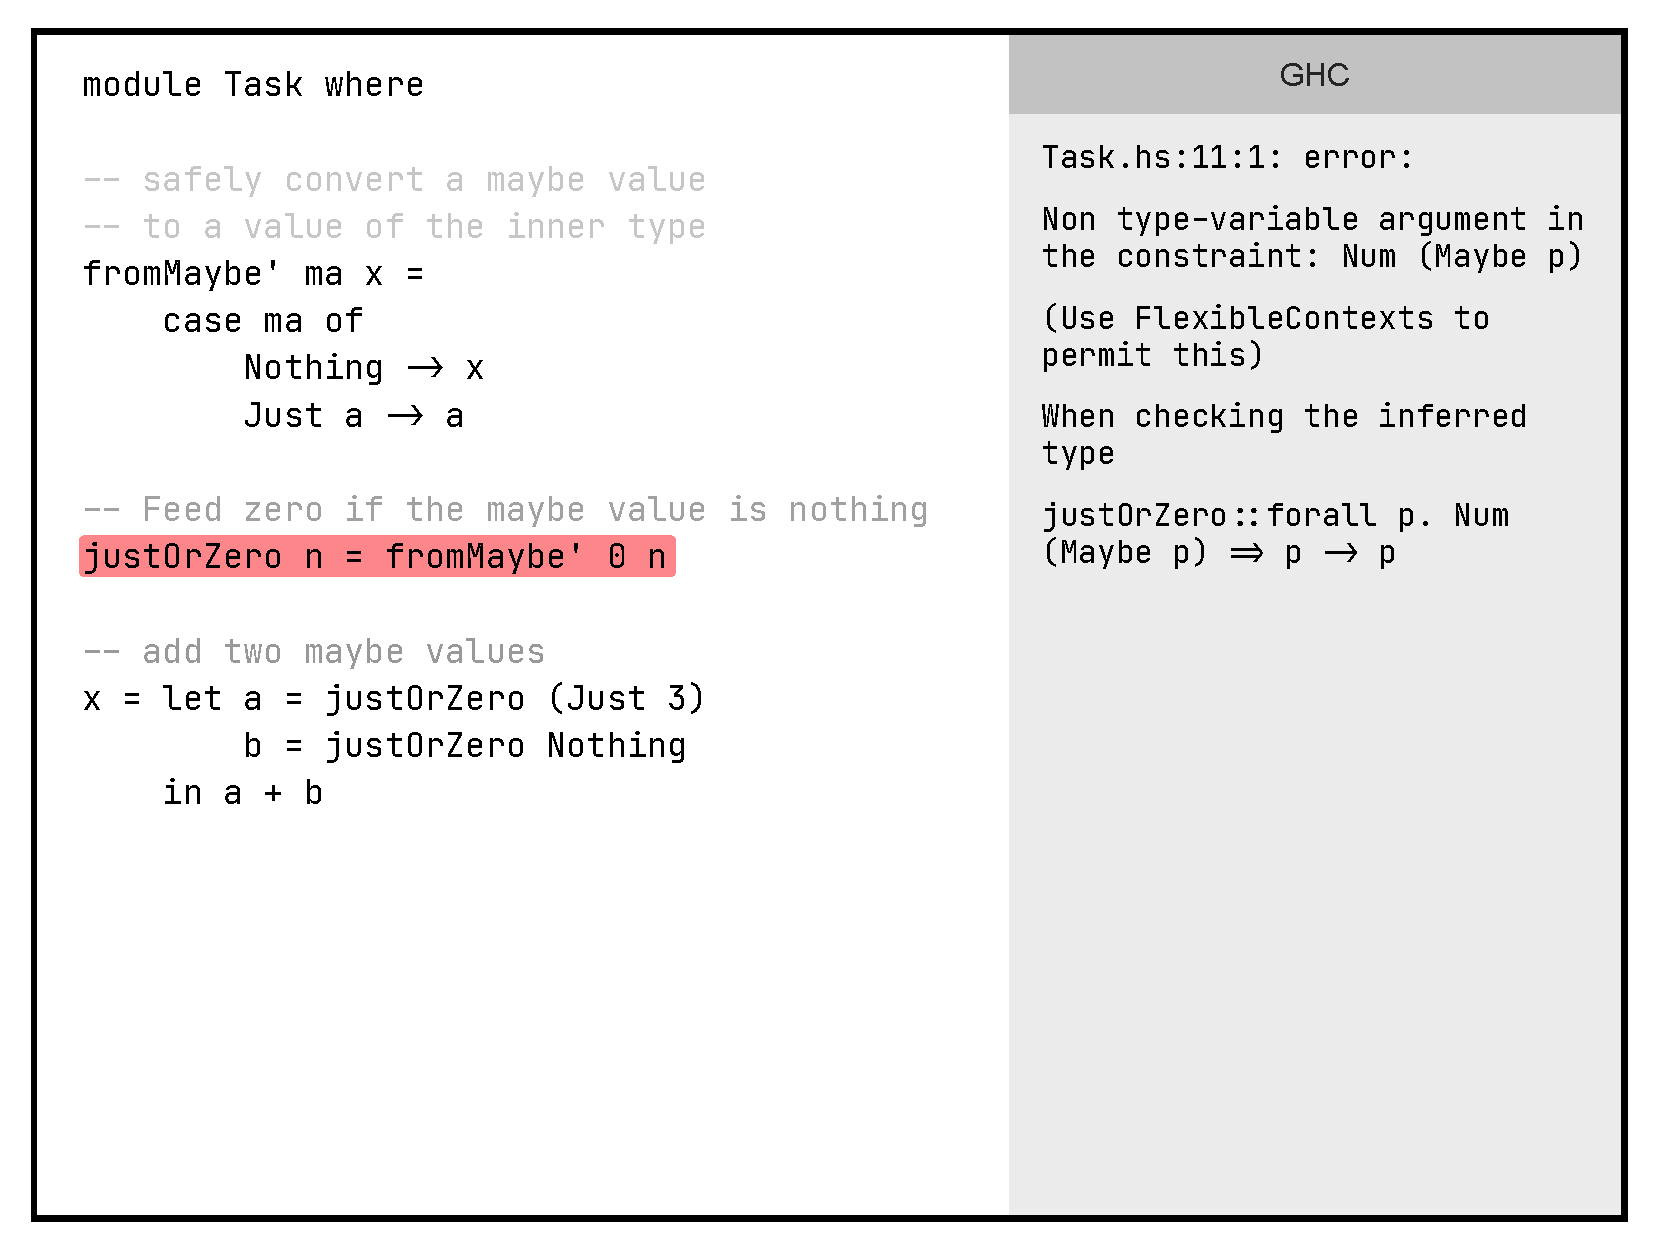
\includegraphics[width=\textwidth]{round1-screenshot-ghc.pdf}
%     \caption{
%         In task 8, participants using GHC took longer pauses at this task before committing to further investigation, either carefully reading the whole text or figuring out the meaning of the error message. The GHC error message is unfortunately unhelpful for this task.
%     }
%     \label{fig:task8-ghc}
% \end{figure}

In comparison, the \chameleon{} group solved the type error faster than the GHC group in almost all tasks (p =0.00742, Wilcoxin signed test) in study 2 (figure \ref{fig:r2-analysis}), barring task 1. The authors are unclear about the cause of low performance from \chameleon{} in task 1. It is suspected that some participants spent more time exploring the interface of \chameleon{} due to its unfamiliarity. From the video recordings, we saw many \chameleon{} users confidently skip reading unrelated chunks of code, while GHC users generally read through the whole program.


In harder problems and messier code, we notice programmers start to report the benefits of \chameleon{}. "Its most useful feature that I noticed was that it points out the locations of both conflicting uses; GHC often makes it difficult to figure out how it's coming to a conclusion about a type." reported one participant. "I think \chameleon{}  does a much better job than GHC's error messages. I like that it shows the sources for the type judgements. This makes it quite easy to figure out how to rectify errors." reported another participant.



\subsubsection{\textbf{Version 2}}  \label{sub:us4}

Version 2 is latest version of \chameleon{}. Not only the added features the deduction steps and candidate expressions are We designed an exploratory study to get better understanding of how users learn and use the multi-mode design of \chameleon{} version 3. During the study the initial mode of each task alternative through the three different modes, and repeat three cycles in nine tasks. The order of the three modes in each cycle is counterbalanced among all participants. However, participants are free to switch to other modes at any time. 



\subsubsection*{\textbf{Results}} 

The study of version 3 \chameleon{} is exploratory, in that we were hoping to let programmers discover their own way of using the tool. In post-hoc analysis of the collected log data, we were able to extrapolate some interesting patterns of how the tool was used. We share a few of our observations in this section.


The most striking feature of the data is users' tendency of using tools differ wildly. That is to say, some users used the feature extensively however some users completed the tasks without actively explore the given information. Based on this difference we divided the users into three groups.

\begin{tabularx}{\linewidth}{ 
  | >{\raggedright\arraybackslash}X 
  | >{\raggedright\arraybackslash}X  | }

    \hline
        Interaction level & Description \\ \hline
        Minimal Interaction & Users completed the tasks by making changes in source code, type checking, and reading error messages. \\ \hline
        Low Interaction & Users only actively used universal features in all modes, for example, hovering on "Possible type 1" and "Possible type 2" to narrow down error space. \\ \hline
        High Interaction & Users did everything from the Common feature group but used features specific to Balanced and Advanced mode, such as activating steps and expression cards. \\ \hline

\end{tabularx}



As shown in  figure \ref{fig:r4-analysis}, the time to complete each task roughly relates to the interaction level of participants. Participants with higher interaction levels generally performed better in the tasks, and the lowest level was worse (one-way ANOVA since we have three samples, p = 0.0368). The results from three tasks stand out from the general trend: in Tasks 4 and 6, higher interaction users performed worse, and in task 9, the general trend is exaggerated. As discussed in user studies 1 and 2, it is likely related to the nature of these tasks. Tasks 4 and 6 are shorter tasks in the study. The ideal fixes for these two tasks are placed relatively early in the source code (both in the first two lines of the source code). These may be useful because following the natural reading order will allow participants to skip lines on the bottom, and thus the advantage of \chameleon{} is less important. On the other hand, task 9 is the longest task of all. It also involves harder problems such as mutually recursive type definitions.

\begin{figure}[h]
    \centering
    \Description{
    Time to complete by task in user study 2 with confidence interval}
    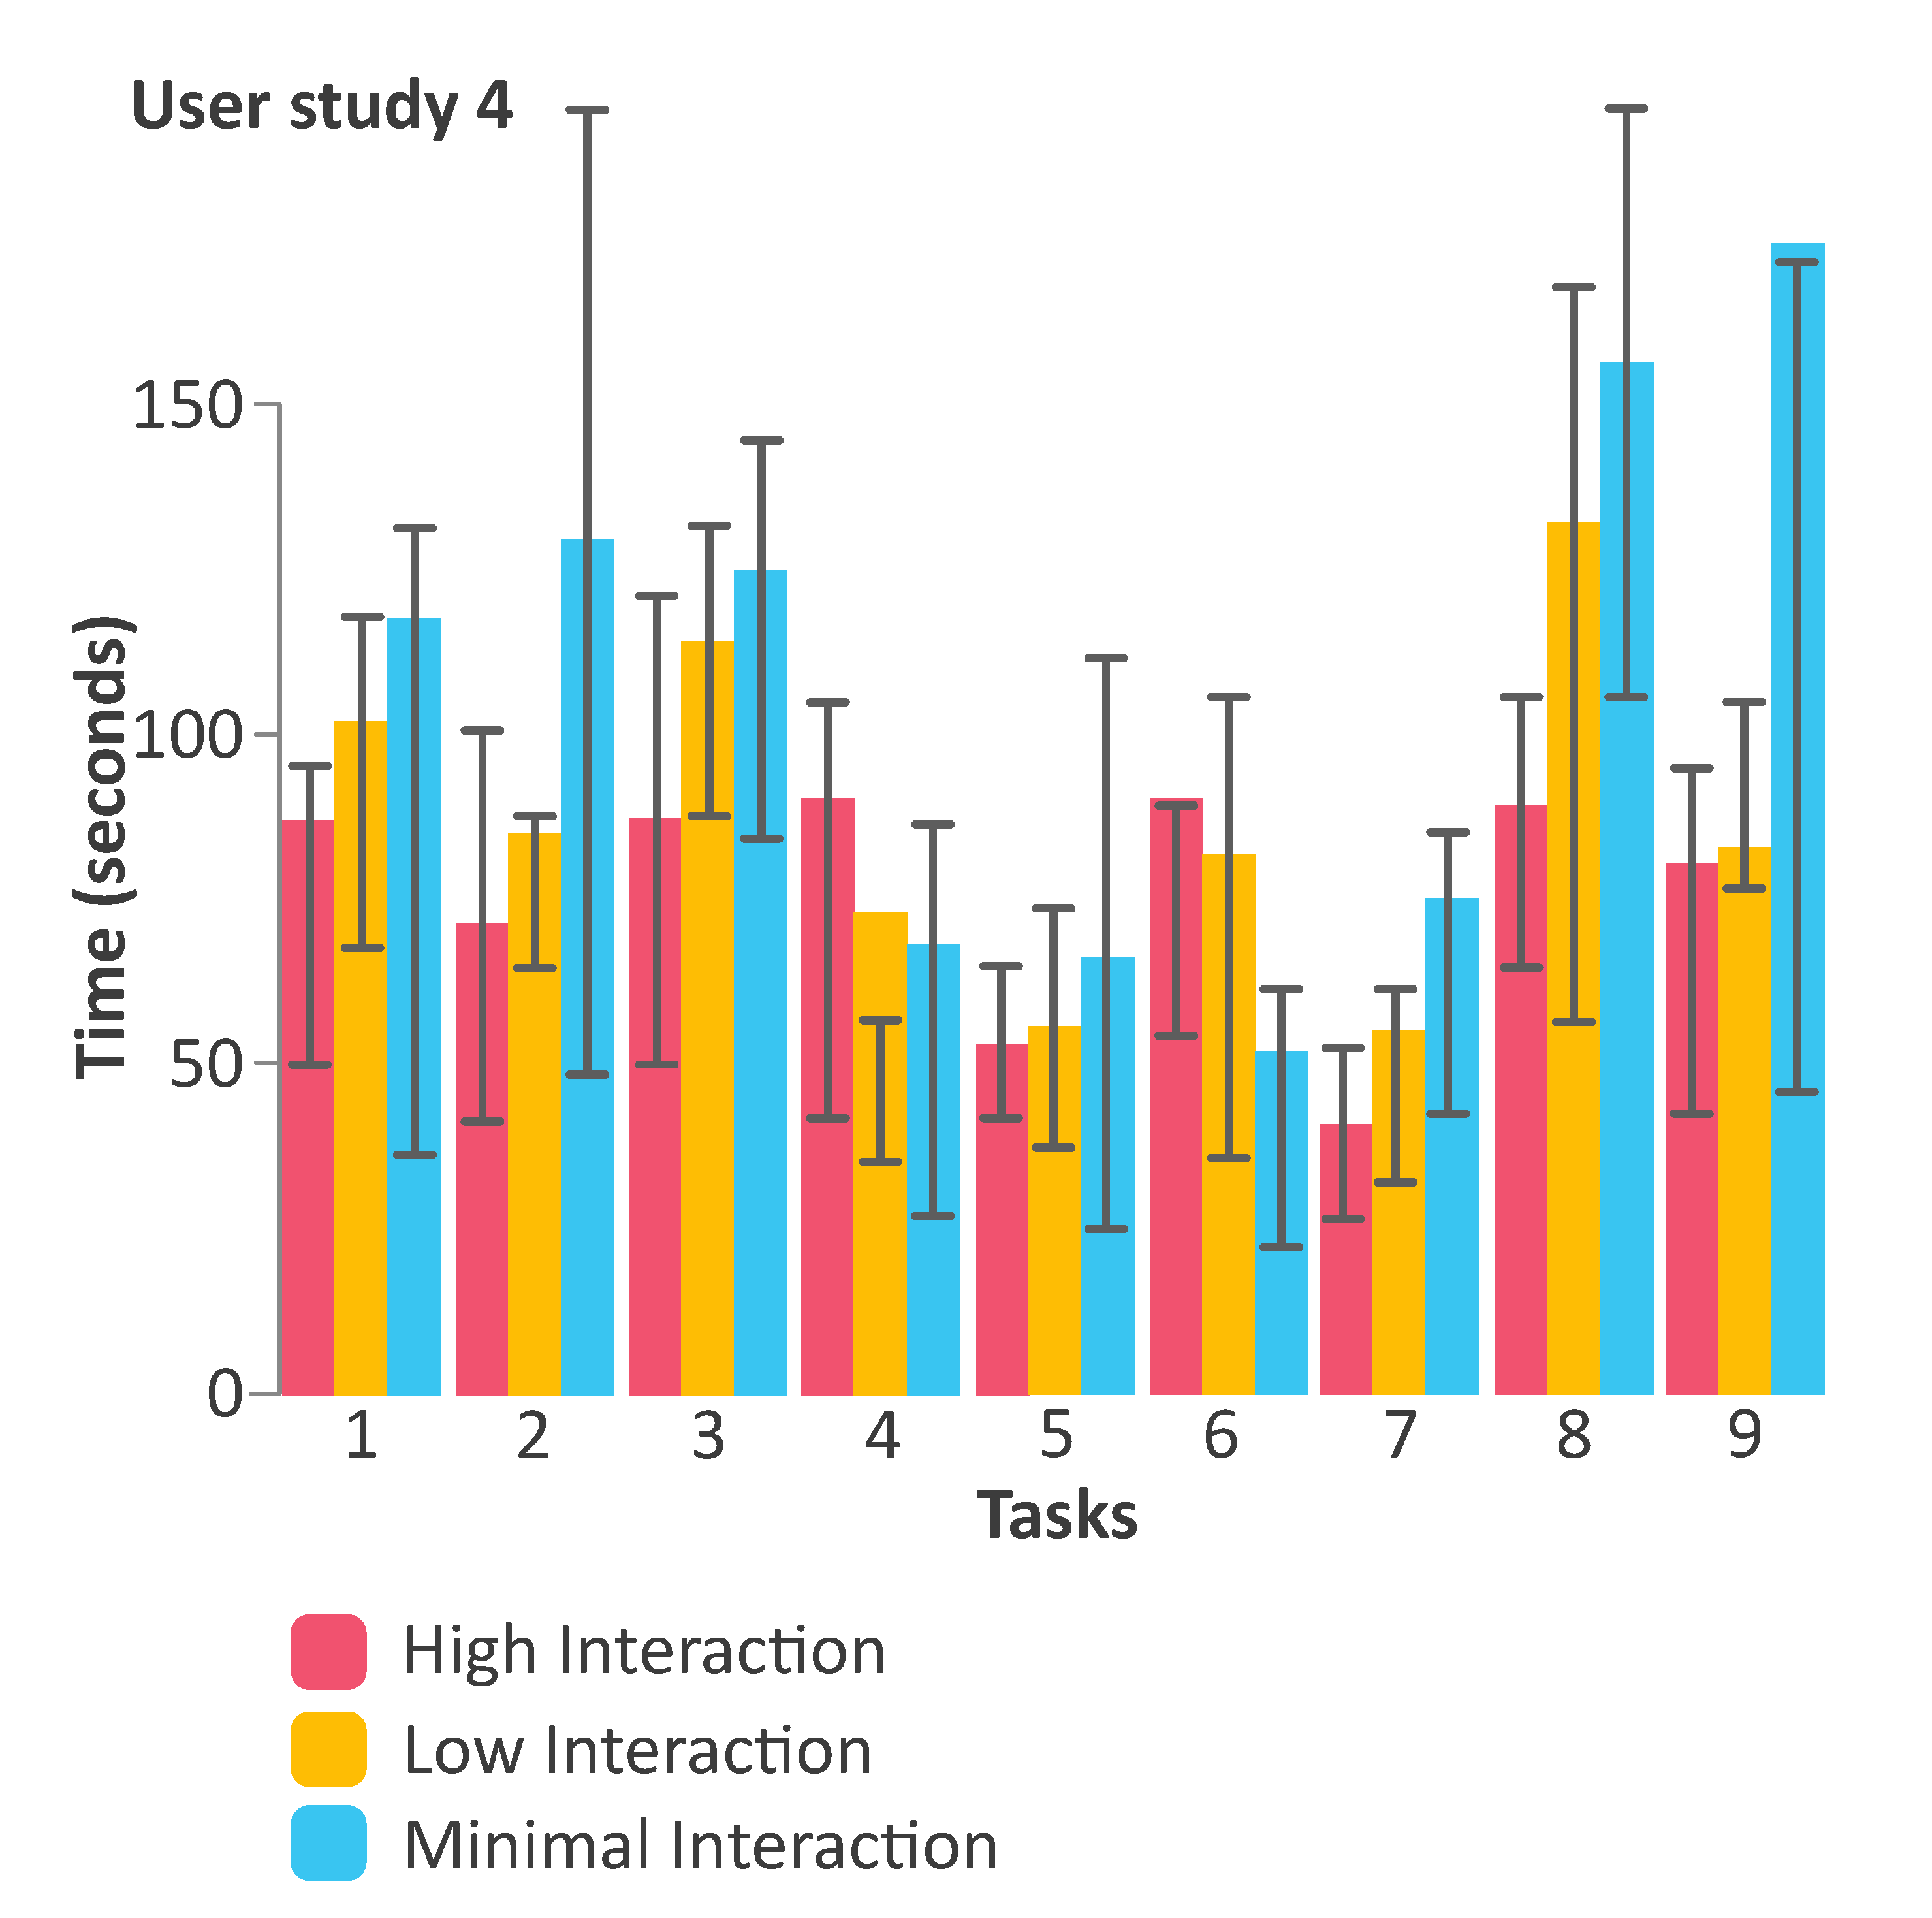
\includegraphics[width=\linewidth]{images/r4-analysis.pdf}
    \caption{Time to complete by task in user study 4 with confidence interval}
    \label{fig:r4-analysis}
\end{figure}


\begin{figure}[h]
    \centering
    \Description{a screenshot from user study for version 2}
    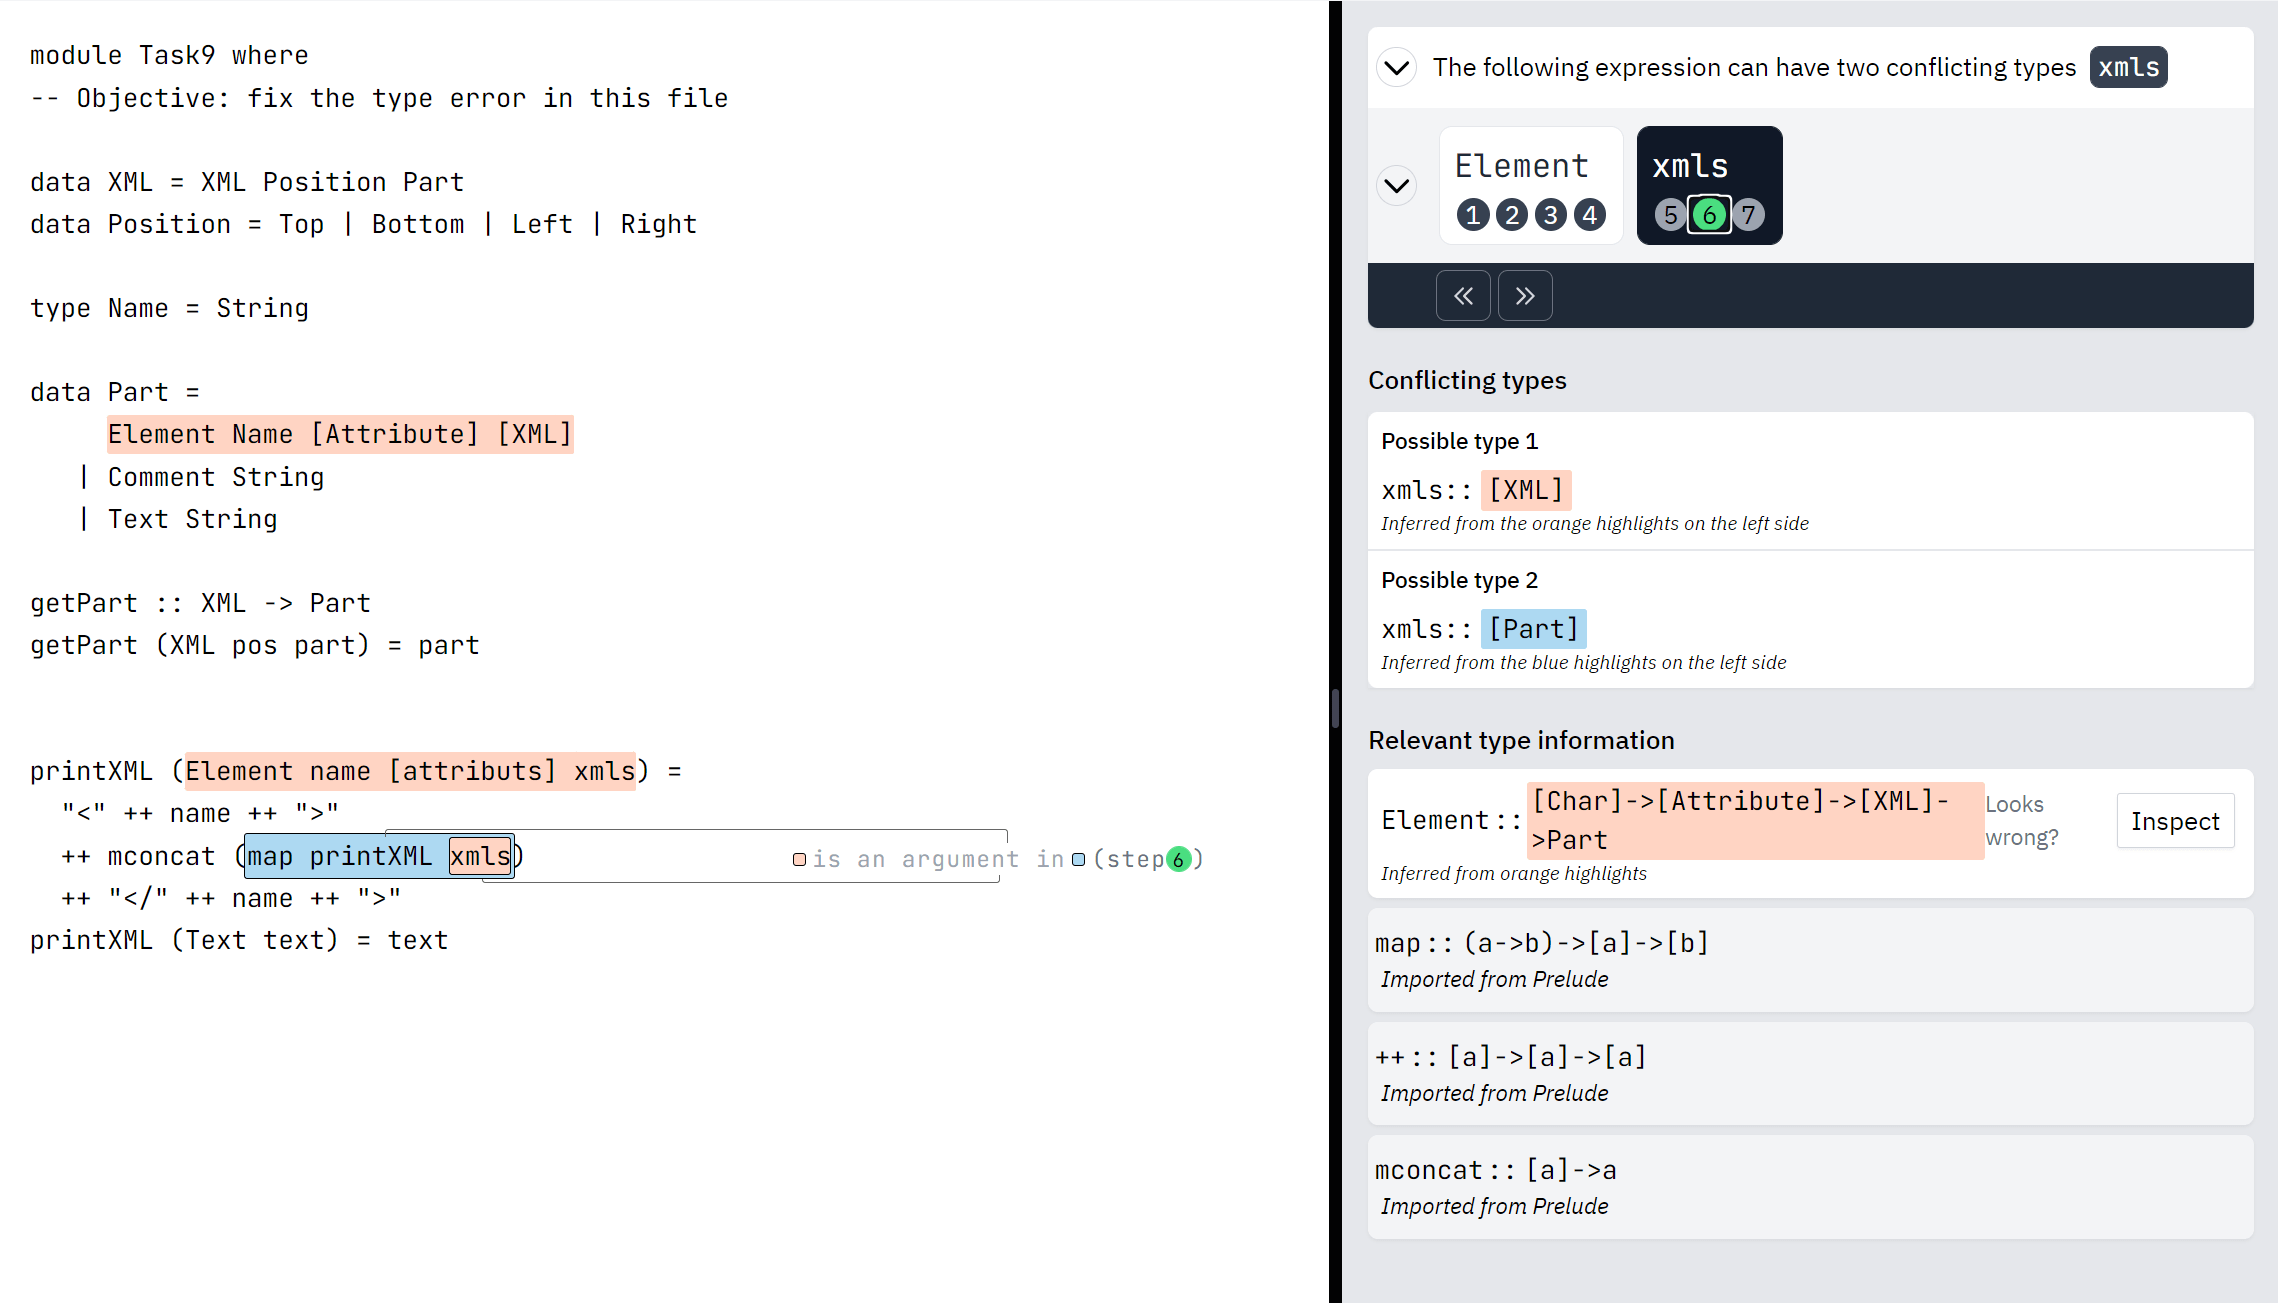
\includegraphics[width=\linewidth]{images/r4-task9.png}
    \caption{
High interaction users were able to locate the exact line for a potential fix after navigating to deduction step 6 or 7, which directly revealed the true cause of the type error. After this, 12 out of 15 high interaction users provided the most ideal fix in the first try. Low interaction group  takes longer time to examine the problem, provided wrong fixes in the initial trials. One participant fixed a minor run-time issue (a problematic pattern matching of `[attributes]` on line 18) however failed to identify the culprit of the type error.
    }
    \label{fig:r4-task9}
\end{figure}


Another observation is when using the mode switching feature of \chameleon{}, programmers generally switching form a less informative display to a more informative one (Fig. \ref{fig:r4-mode-switching}). 

\begin{figure}[h]
    \centering
    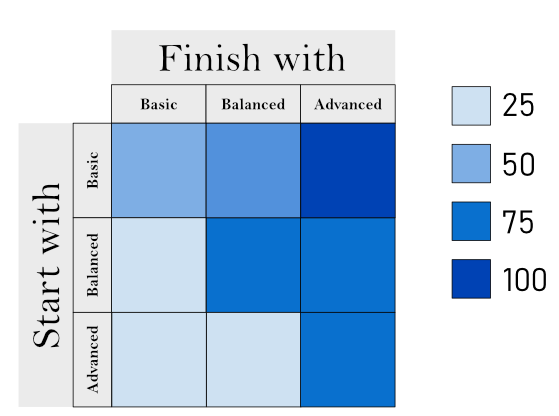
\includegraphics[width=\linewidth]{images/r4-mode-switching.png}
    \caption{
        \textbf{Row Number of tasks }
    
    }
    \label{fig:r4-mode-switching}
\end{figure}



\section{Discussion}

% \todo{Suggest try and strucuture this a bit more e.g. each para bold the key lesson @ start of para. Can you group into implications for research/implications for practice to make more actionable??}

This paper presents the interactive type debugging tool \chameleon{} and charts the evolution of its design across several iterations in response to user evaluation and feedback, as well as examining the effectiveness of the general approach compared to traditional static type error messages. We found that programmers using \chameleon{} type compare tool are able to debug errors faster than using traditional text-based error messages. This effect is shown more clearly when the task is not trivial. We found that programmers who actively use \chameleon{}'s interactive features (candidate expression cards and deduction steps) are more efficient in fixing type errors than passively reading the type error output. In this section, we will discuss a few interpretations of the results.


\subsection{Effect on Reading Source Code}
From the results of Study 1a, we observed that the choice of debugging tool had little effect on how fast programmers solve simple type errors. Conversely, when facing more realistic problems (longer source code, error locations more scattered) in study 1b, programmers are more effective using \chameleon{}. One explanation is that \chameleon{} reduces the amount of reading time by taking programmers more directly to the problem. Earlier studies \cite{jbara_how_2015, peitek_what_2020} showed that reading source code is generally the initial step of solving programming problems and is done in several passes. Although traditional compiler error message tools initially show fewer locations, these may be incomplete, meaning that programmers have to expand the reading span without clear guidance. In contrast, Chameleon shows more error locations initially. However, the completeness of error locations assures programmers which part of the source code can be safely skipped.

\subsection{Forming Debugging Plans}
From the results of Study 2, we found that programmers who use the interactive tool fix type errors faster than the ones who passively read the error output. This effect is stronger in harder tasks. We speculate that one factor of this result is that  \chameleon{} helps to develop debugging plans. We observed that when working with \chameleon{}, programmers form different debugging tactics to attack the problem. Among the \textit{high} interactivity participants in user study 4, some programmers cycle through deduction steps as a guide to reading source code; some programmers navigate to both ends of the deduction steps where types are normally grounded and concrete. In contrast, \textit{minimal} interactive participants generally form similar plans, including carefully reading the program text and manually annotating expressions based on their understanding of the program.


\subsection{Externalize Intermediate Typing Information}
We speculate another factor of the effectiveness \chameleon{} interactive debugging tools is they help programmers effectively chunk intermediate information. With the program shown in Listing~\ref{listing:2}, \chameleon{} offers two candidate expressions: \texttt{f} can be typed as \texttt{Int -> Bool} or \texttt{Char -> Bool}; \texttt{z} can be typed as \texttt{Int} or \texttt{Char}. Although  these two statements are equivalent in theory, programmers are often required to compute the latter from the former or vice versa. And this computation may carry out multiple layers. Programmers have to remember all the intermediate types and their reasoning throughout such mental gymnastics. Assisted by candidate expression cards and deduction steps, this intermediate information is externalized on screen and can be retrieved anytime. A recent study on working memory \cite{crichton_role_2021} suggested this approach may provide a positive effect in helping programmers manage cognitive load and free up working-memory space for high-level thinking.

\begin{listing}
\begin{minted}{haskell}
f z     
    | z == 3 = False
    | z == '4' = True
\end{minted}
\caption{In this simple program, \chameleon{} reports the error happened in \texttt{f} and \texttt{z}.}
\label{listing:2}
\end{listing}
% Implication for research
% In our studies, \chameleon{} shows a few different designs for type error visualization and interaction. However, we are far from exhausting the search space. One challenge we notice in the current design is that programmers have to shift their focus between the editor on the left and the \chameleon{} debugging interface on the right. Using the hover popup window in most mainstream IDEs may reduce the context switching during debugging.

% Integration with existing tools
% The current implementation of \chameleon{} requires non-trivial adaptation for editors such as VS Code and IntelliJ due to the overlay explanation layer. This type of error visualization is non-standard in mainstream editors. However, there may exist alternative representations of \chameleon{} error reporting using only the features available in major editors and IDEs. It is especially beneficial to represent \chameleon{} errors using a universal debugging middle layer such as language server protocol (LSP). This will allow \chameleon{}  to be adapted into various coding environments which support an LSP back end.


% Extend to other languages
% Our study focuses on the Haskell language for its popularity in the academic world. However, the low quality of textual type errors is a problem not limited to Haskell. Modern statically typed languages more or less all share the same problem. We believe the underlying type reporting technique and algorithms can be generalized to other languages. It will be exciting to see how interactive debugging features perform in other paradigms, such as  imperative languages and incremental type systems.

% Ranking candidate expressions and alternative types
% Our design of \chameleon{}  emphasizes allowing programmers to update the type error based on their prior knowledge. It unfolds to answer three questions: which expression should be considered ill-typed? Between multiple possible types, which one should be considered intended? Among all the possible locations, which one should be considered the cause? \chameleon{} answers all three questions by leaving them to the hands of the programmers. However, it is possible in situations, prescriptive error messages are preferred. Using heuristic methods may achieve the best of both worlds. It may produce effective results by guessing the possible un-typable expression based on the position it appears in the syntax tree and project structure or guessing the intended type signature by comparing the number of supporting slices in the source code.


\section{Conclusion}

We present \chameleon{}, a type debugging tool for the Haskell programming language. Its constraint-based type inference engine provides unbiased and comprehensive error location reporting. 
% This sentence could go away:
%\chameleon{} also features an interactive debugging interface with three debugging modes, enabling programmers to interactively explore the stepwise explanations. 
Our studies evaluated the tool's design with programmers. We found that, particularly for more complex tasks, \chameleon{} helped programmers to fix type errors more quickly than traditional text-based error messages. Further, programmers actively using \chameleon{} interactive features are shown to fix type errors faster than simply reading the type error output.
\chameleon{} currently works with the Haskell language, but in the future, we plan to extend the type-checking system to work with other strongly typed languages, such as Rust or TypeScript.

\subsection*{Acknowledgments} 

The work of Peter Stuckey was partially supported by the OPTIMA ARC ITTC, Project ID IC200100009.

\goodbreak\noindent



\bibliographystyle{IEEEtran}
\bibliography{icpc}


\end{document}
